
\documentclass[a4paper, fleqn, usenatbib, useAMS]{mnras}
\usepackage[T1]{fontenc}
\usepackage{ae, aecompl}			% Required for MNRAS
\usepackage{newtxtext, newtxmath} 	% Required for MNRAS 
\usepackage{mathtools}
\usepackage{graphicx}
\usepackage{amsmath}
\usepackage{amssymb}
\usepackage{multicol}
\usepackage{bm}
\usepackage{pdflscape}
\usepackage{natbib}
\usepackage[section]{placeins}
\usepackage{lipsum}
\usepackage{etoolbox} 
\usepackage{tabularx} 
\usepackage{xcolor} 
\usepackage[toc, page]{appendix} 
% \hypersetup{draft} 
\hypersetup{ 
	colorlinks		= true, 
	urlcolor 		= blue, 
	linkcolor 		= blue, 
	citecolor 		= blue 
} 

\newcommand{\ddfrac}[2]{\frac{\displaystyle #1}{\displaystyle #2}} 
\newcommand{\refp}[1]{(\ref{#1})} 
\graphicspath{ {../plots/} } 

\interfootnotelinepenalty = 10000 
\defcitealias{Kroupa2001}{Kroupa} 
\defcitealias{Salpeter1955}{Salpeter} 

% \title[The Pivotal Role of Radial Migration]{The Pivotal Role of Radial 
% Migration in the Chemical Enrichment of the Milky Way} 
% \title[Galactic Archaeology with Stellar Migration]{Galactic Archaeology with 
% Stellar Migration} 
\title{Stellar Migration and Chemical Enrichment in the Milky Way} 

\author[J.W. Johnson et al.]{
	James W. Johnson,$^{1}$\thanks{Contanct e-mail: \href{mailto:
	johnson.7419@osu.edu}{johnson.7419@osu.edu}} 
	David H. Weinberg,$^{1, 2}$ 
	Fiorenzo Vincenzo,$^{2}$ 
	Jonathan C. Bird,$^{3}$ 
	\newauthor 
	Sarah R. Loebman,$^{4}$ 
	Alyson Brooks,$^{5}$ 
	Thomas R. Quinn,$^{6}$ 
	Charlotte R. Christensen,$^{7}$ 
	\newauthor 
	et al.?
	\\
	$^{1}$ Department of Astronomy, The Ohio State University, 
	140 W. 18th Ave., Columbus, OH, 43210, USA 
	\\ 
	$^{2}$ Center for Cosmology and Astroparticle Physics (CCAPP), 
	The Ohio State University, 191 W. Woodruff Ave, Columbus, OH, 43210, USA 
	\\ 
	$^{3}$ Department of Physics \& Astronomy, Vanderbilt University, 
	2301 Vanderbilt Place, Nashville, TN, 37235, USA 
	\\ 
	$^{4}$ Department of Physics, University of California Merced, 
	5200 North Lake Rd., Merced, CA, 95343, USA 
	\\ 
	$^{5}$ Department of Physics \& Astronomy, Rutgers University, 136 
	Frelinghuysen Rd, Piscataway, NJ, 08854, USA 
	\\ 
	$^{6}$ Department of Astronomy, University of Washinton, Box 351580, 
	Seattle, WA, 98195, USA 
	\\ 
	$^{7}$ Department of Physics, Grinnell College, 1116 8th Ave., Grinnell, 
	IA, 50112, USA 
} 

\date{Accepted XXX; Received YYY; in original form ZZZ} 
\pubyear{2020} 

\begin{document} 
\label{firstpage} 
\pagerange{\pageref{firstpage}--\pageref{lastpage}} 
\maketitle 

\begin{abstract} 
We investigate the impact of stellar migration on galactic chemical evolution 
models, considering a handful of assumptions for the star formation history 
and time-dependence of radial migration based on a zoom-in, hydrodynamical 
N-body simulation of galaxy evolution. To this end, we extend the 
\texttt{Versatile Integrator for Chemical Evolution} (\texttt{VICE}), 
developing and making use of its~\texttt{milkyway} object, built to handle 
these models under a wide variety of assumptions. We find that models for the 
time-dependence of radial migration impact the type Ia supernova rate as a 
function of both time and radius, inducing significant variability. We 
demonstrate that this is a means with which young, $\alpha$-enhanced stars can 
arise naturally out of inside-out galaxy growth with stellar migration. We find 
that the observed age-[$\alpha$/Fe] relation is well-fit by an inside-out star 
formation history, while the age-[O/H] and age-[Fe/H] relations are well-fit by 
a late starburst model; no one model investigated here fits both 
simultaneously. Lastly, we find that none of our models predict an 
[$\alpha$/Fe] dichotomy resembling that observed in the Milky Way. This 
suggests that inside-out galaxy growth combined with radial migration, even 
with a late starburst, is not conducive to forming the infamous bimodality. 
We postulate that more dramatic evolutionary events (e.g. a two-infall model) 
are necessary to describe the observed results.~\texttt{VICE} is publicly 
available at~\url{https://pypi.org/project/vice}. 
\end{abstract} 

\begin{keywords} 
methods: numerical -- galaxies: abundances, evolution, star formation, stellar 
content 
\end{keywords}

\section{Introduction} 
\label{sec:intro} 
\begin{itemize} 
	\item The Age-Metallicity Relation (AMR) 
	\begin{itemize} 

		\item Known for some time that stars undergo radial migration, 
		but to date there are only a handful of chemical evolution models that 
		take this into account~\citep{Wielen1996, Edvardsson1993, Sellwood2002, 
		Schoenrich2009, Minchev2013, Minchev2014, Minchev2017, Sharma2020}. 

		\item Age-metallicity relation in the solar neighbourhood exhibits 
		considerable intrinsic scatter~\citep{Edvardsson1993}, usually 
		attributed to radial migration of metal-rich (metal-poor) stars formed 
		at smaller (larger) Galactocentric radii~\citep{Sellwood2002, 
		Haywood2008, Roskar2008b, Schoenrich2009}. 

		\item \citet{Feuillet2018} reveal that super-solar metallicity stars 
		are statistically older than solar metallicity stars (their Fig. 3). 
		Contrasts with simple one-zone models where enrichment proceeds 
		alongside star formation yielding a monotonic 
		AMR~\citep[e.g.][]{Andrews2017, Weinberg2017}. One-zone models of 
		starbursts can produce non-monotonic AMR due to the effect of 
		dilution~\citep{Johnson2020}, but they by construction do not predict 
		multiple abundances at fixed age. 
	\end{itemize}

	\item The Young Alpha-Rich Population 
	\begin{itemize} 
		\item Population of young ($\sim$few Gyr), [$\alpha$/Fe]~$\sim$ 
		0.1-0.2 stars in the solar neighbourhood. 

		\item Found using stellar ages estimated carbon-to-nitrogen 
		ratios~\citep{Martig2016}, isochrone matching~\citep{Feuillet2018, 
		Feuillet2019}, and with the asteroseismic ages in the original APOKASC 
		catalog~\citep{SilvaAguirre2018, Pinsonneault2014}. 

		\item \citet{Mor2019} infer a factor of~$\sim$2 enhancement in the 
		SFH of the Milky Way~$\sim$2 Gyr ago by comparing population synthesis 
		models to observed stellar luminosity functions and color-magnitude 
		diagrams from Gaia data~\citep{GaiaDR2}.~\citet{Isern2019} reach 
		similar conclusions by modeling the white dwarf luminosity function in 
		the solar neighbourhood with Gaia parallaxes. Motivated by these 
		results, \citet{Johnson2020} demonstrate using one-zone chemical 
		evolution models that a recent starburst can produce young, 
		$\alpha$-enhanced stars. Caveat: burst would have had to be 
		sufficiently localized such that the young,~$\alpha$-rich stars remain 
		outliers from an otherwise monotonically descreasing age-[$\alpha$/Fe] 
		relation. 
	\end{itemize} 

	\item The [$\alpha$/Fe] bimodality 
	\begin{itemize} 
		\item Milky Way stars segregate themselves into the low- and 
		high-$\alpha$ sequences, a bimodality found in, e.g., 
		Gaia ESO~\citep{Recio-Blanco2014, Rojas-Arriagada2017}, and 
		APOGEE~\citep{Nidever2014, Hayden2015, Weinberg2019}. 

		\item Presence is well established, though origin a topic of intense 
		debate. 

		\item Notion that it could arise out of radial migration traces back 
		to~\citet{Schoenrich2009}. 

		\item \citet{Weinberg2017} models suggest increase in strength of the 
		mass-loading factor $\eta$ at late times would lower the equilibrium 
		abundance, forming stars along the low-$\alpha$ sequence. This plus 
		radial migration is yet unexplored. 

		\item \citet{Spitoni2019} demonstrate that two-infall models can 
		reproduce solar annulus data with good agreement. This plus 
		radial migration is yet unexplored. 

		\item \citet{Grand2018} find with Auriga~\citep{Grand2017} that early, 
		accretion induced starburst populates the high-$\alpha$ sequence, 
		followed by low-level, sustained star formation on low-$\alpha$ 
		sequence, and a rapid transition between the two ensures chemical space 
		relatively unpopulated. This would imply short $\tau_\star$ (see 
		justification in~\citealp{Weinberg2017}). Ongoing, low-metallicity 
		gas accretion can also populate low-$\alpha$ sequence.~\citet{Buck2020b} 
		find results qualitatively similar to second scenario in NIHAO 
		simulation suite~\citep{Wang2015, Buck2020a}. Hydrodynamical 
		simulations take into account radial migration by construction. 

		\item \citet{Clarke2019} show that star formation proceeded in clumps 
		in an SPH simulation of an NFW halo using GASOLINE~\citep{NFW1997, 
		Wadsley2017}. The clumps self-enrich, forming stars on the 
		high-$\alpha$ sequence, while more spatially extended, smooth star 
		formation populated the low-$\alpha$ sequence. 

		\item No shortage of models that reproduce the dichotomy, yet only 
		those done with hydrodynamical simulations and a handful of others 
		have taken into account radial migration. 
	\end{itemize} 

\end{itemize} 

\section{Data and Methods} 
\label{sec:methods} 

\begin{itemize} 
	\item This paper is meant to address the simple question of: ``When 
	combining simple, realistic assumptions about the star formation and 
	dynamical histories of the Milky Way, what observed results can be 
	replicated?'' 
\end{itemize} 

\subsection{Multi-Zone models} 
\label{sec:methods:multizone} 
\begin{itemize} 
	\item Multizone models are a means of extending traditional one-zone 
	models to take into account the motions of stars and gas by allowing the 
	exchange of both between zones. 

	\item Qualitatively similar approach in~\citet{Matteucci1989, 
	Schoenrich2009, Minchev2013}. 

	\item \texttt{VICE} released in~\citet{Johnson2020}, presented first 
	results from~\texttt{singlezone} object. Develop the~\texttt{multizone} 
	object and the~\texttt{milkyway} extension of that, and make use of them 
	here.~\texttt{multizone} simply provides an array of~\texttt{singlezone} 
	objects and allows the exchange of gas and individual stellar populations 
	between any two zones at any given simulation time.~\texttt{milkyway} 
	forces an annular model, where here we take a width of 100 pc, and 
	adopts by default the migration scheme discussed in the next subsection. 

	\item Don't go into gory detail here, but provide a brief summary 
	of~\texttt{VICE}'s algorithm. Further details can be found in the 
	science documentation. 
	\begin{itemize} 
		\item At it's core, the~\texttt{multizone} object is an array 
		of~\texttt{singlezone} objects, each with its own ISM mass, star 
		formation rate, and infall rate.~\texttt{multizone} migration 
		prescriptions describe how gas and stars move between zones. Gas can be 
		moved between any pair of zones according to user-constructed functions 
		of time. Stars are stand-ins for entire stellar populations, and the 
		user has full control over what zone every single stellar population 
		is in at every single timestep. This should allow arbitrarily complex 
		zone schema to be implemented. Hydrodynamical simulations form varying 
		numbers of star particles of fixed mass, but~\texttt{VICE} forms a 
		fixed number of stellar populations per zone per timestep, each with a 
		mass that is simply~$\dot{M}_\star\Delta t / n$ where~$\dot{M}_\star$ 
		is the star formation rate, $\Delta t$ is the timestep size, 
		and~$n$ is the number of stellar populations per zone per timestep. 

		\item \texttt{milkyway} object extends the~\texttt{multizone} object 
		and assumes an annular zone configuration, automatically adopting the 
		migration schema from this paper as a default. There is thus a fixed 
		number of stellar populations per annulus per timestep. 
	\end{itemize} 
\end{itemize} 

\subsection{Radial Migration} 
\label{sec:methods:migration} 
\begin{itemize} 
	\item Algorithm based on initial and final radii of star particles in 
	hydrodynamical simulations. 

	\item Stellar populations assumed to be born at centres of their annuli. 
	For a stellar population born at time $T$ and Galactocentric radius 
	$R_\text{gal}$,~\texttt{VICE} searches for star particles formed at 
	$T \pm$ 300 Myr and $R_\text{gal} \pm$ 250 pc. It then randomly selects 
	a star particle from this subsample with no bias to act as 
	an~\textit{analog}. Adopts the final radius of the star particle at face 
	value, and moves from its radius of birth to the final radius at $T$ = 
	12.7 Gyr with some time dependence. If no candidate analogs are found, 
	search is widened to $T \pm$ 600 Myr and $R_\text{gal} \pm$ 500 pc. If 
	still no candidate analogs are found in this widened search, the stellar 
	population is assumed to remain at its birth radius {\color{red} and to 
	have a final height above the disk midplane of $z$ = 100 kpc.} These 
	stellar populations are few in number. 
	\begin{itemize} 
		\item We have zones only for each annulus from $R_\text{gal}$ = 0 to 
		20 kpc; there are no zones off the midplane, retaining the assumption 
		that the gas-phase abundances are vertically well mixed as well as 
		azimuthally. Each stellar population simply assumes the final height 
		$\left|z\right|$ of its assigned analog, though this doesn't enter 
		into the simulations at all; it's purely post-processing information. 
	\end{itemize} 

	\item When a star particle is assigned as an analog to a stellar 
	population in our simulations, it is~\textit{not} thrown out of the sample 
	of candidate analogs, allowing star particles to in theory act as analogs 
	for multiple stellar populations. This is a difference between 
	the~\citet{Minchev2013} model and ours. 

\begin{figure} 
\centering 
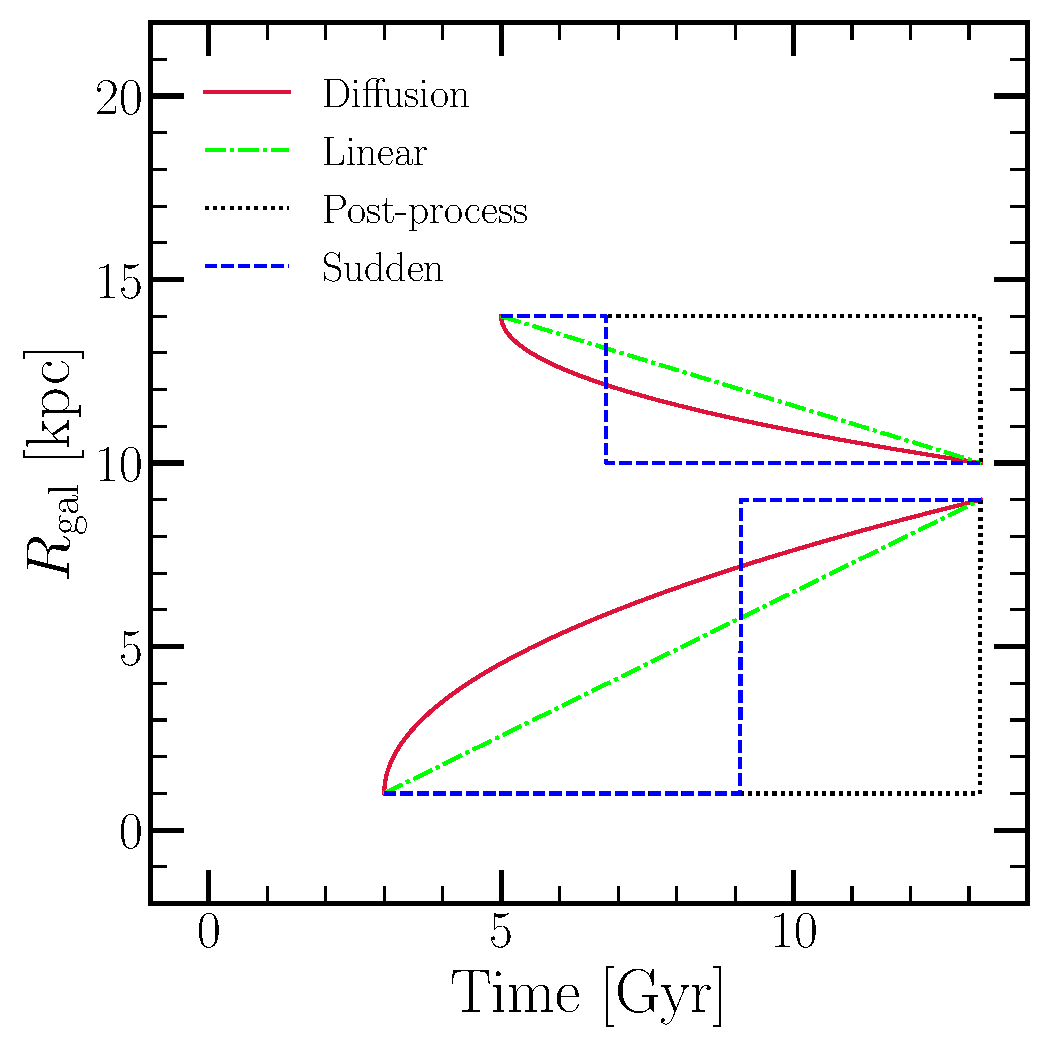
\includegraphics[scale = 0.45]{migration.pdf} 
\caption{A diagram illustrating how Galactocentric radius changes with time 
for three stellar populations under our migration schema: diffusion (crimson, 
solid), linear (lime, dot-dashed), post-process (black, dotted), and 
sudden (blue, dashed). Here the initial and final radii and birth times are 
pseudorandom numbers drawn from a uniform distribution for illustrative 
purposes. With the initial and final Galactocentric radii of a stellar 
population, its birth time, and one of these assumptions about the 
time-dependence of migration, the Galactocentric radius at all times is 
known. } 
\label{fig:migration_schema} 
\end{figure} 

	\item Our migration models 
	\begin{itemize} 
		\item All neglect radial gas flows, this paper instead focusing on 
		four simple models for how the radius of a stellar population's orbit 
		changes with time. Investigation of our models with radial gas flows 
		would be an interesting extension to this paper. 

		\item \textbf{Post-processing}: Stars stay where they are born until 
		the final timestep. Based on the assumption that stellar populations 
		do not contribute to enrichment beyond their birth 
		radius~\citep[e.g.][]{Minchev2013}. Each annulus simulated as a 
		one-zone model independent of all other zones. Shown in black dotted 
		line in Fig.~\ref{fig:migration_schema}. 

		\item \textbf{Sudden}: A random number is drawn from a uniform 
		distribution between the time of birth and the present day. That time 
		is taken to be the time of instantaneous migration ot the present-day 
		annulus. Emulates a scenario in which a single dynamical interaction 
		changes the orbital radius of a star. Can be thought of as a 
		time-dependent extension of the post-processing scenario. Shown in 
		blue dashed line in Fig.~\ref{fig:migration_schema}. 

		\item \textbf{Diffusion}: Continuous, time-dependent migration with a 
		$\sqrt{\text{age}}$ dependence. Emulates a scenario in which angular 
		momentum diffuses throughout the disk via a random walk, in which 
		case the mean displacement of a star from its birth radius would 
		scale with $\sqrt{t}$. Shown in red solid line in 
		Fig.~\ref{fig:migration_schema}. 

		\item \textbf{Linear}: A simple time-dependent variation of the 
		diffusion model. Has no physical motivation other than numerical 
		ease, but together with the diffusion model constitutes a test of how 
		sensitive our models are to the assumed time-dependence of radial 
		migration. Demonstrated by green dot-dashed line in 
		Fig.~\ref{fig:migration_schema}. 
	\end{itemize} 
\end{itemize} 

\subsection{The Hydrodynamical Simulation} 
\label{sec:methods:h277} 

\begin{figure} 
\centering 
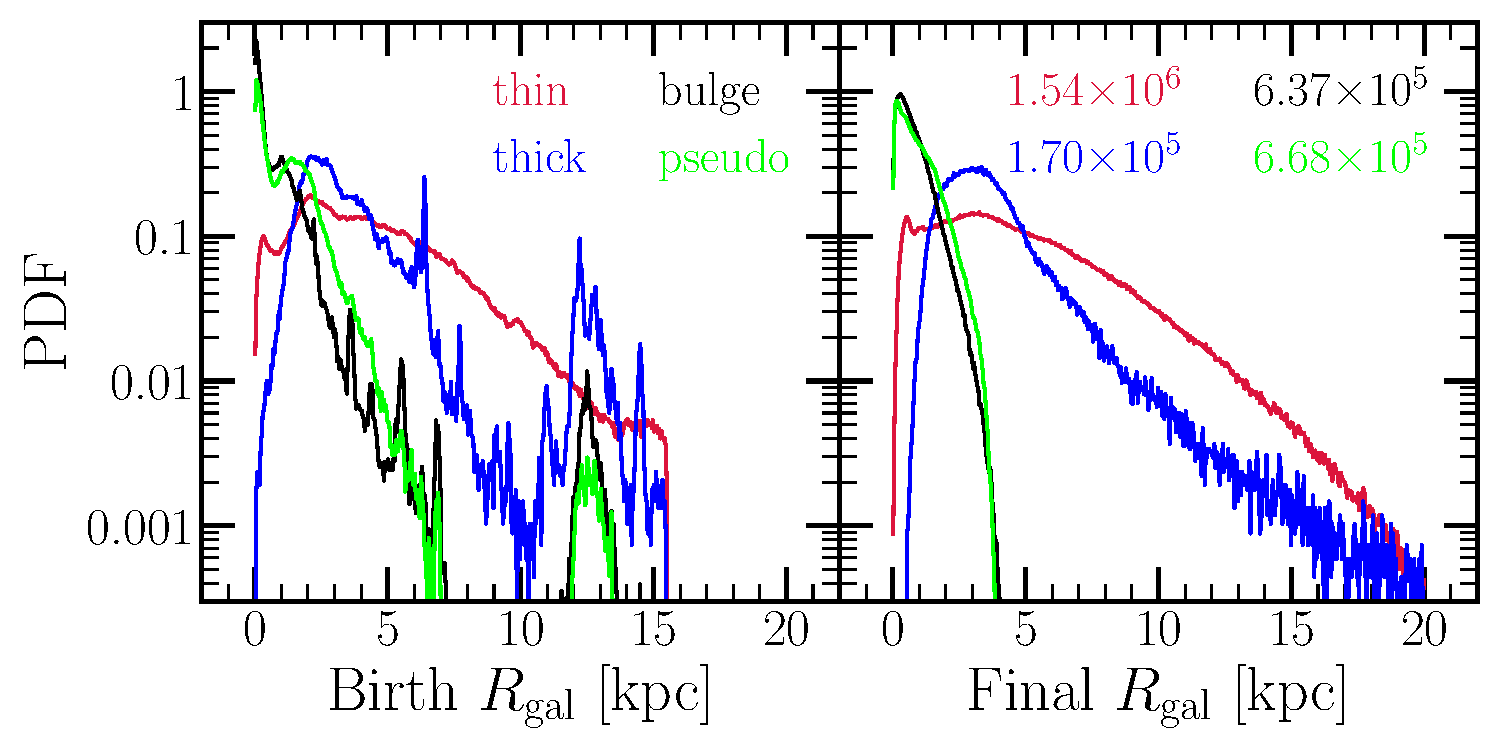
\includegraphics[scale = 0.32]{birth_final_radii_pdfs.pdf} 
\caption{Distributions of~\texttt{h277} star particles in their birth (left) 
and final (right) Galactocentric radii. Distributions are shown for thin 
disk (crimson), thick disk (blue), bulge (black), and pseudobulge (lime) 
populations according to the kinematic decomposition described in~\S~X. 
In the right-hand panel we denote the number of star particles in each 
population according to the same color-coding. {\color{red} I cut off 
$R_\text{Form}$ at 15.5 kpc in my reduction from Jon's file of star 
particles. Extend it to 20 kpc, just for the sake of having candidate analogs 
out there for future papers? We can still cut off star formation here at 
15.5 kpc, so any stars that form out there and migrate inward will have zero 
mass and thus no effect, but maybe worth it for showing the distributions. 
I'd only have to change one line of code and rerun things. }} 
\label{fig:h277_birth_final_radii_pdfs} 
\end{figure} 

\begin{figure*} 
\centering 
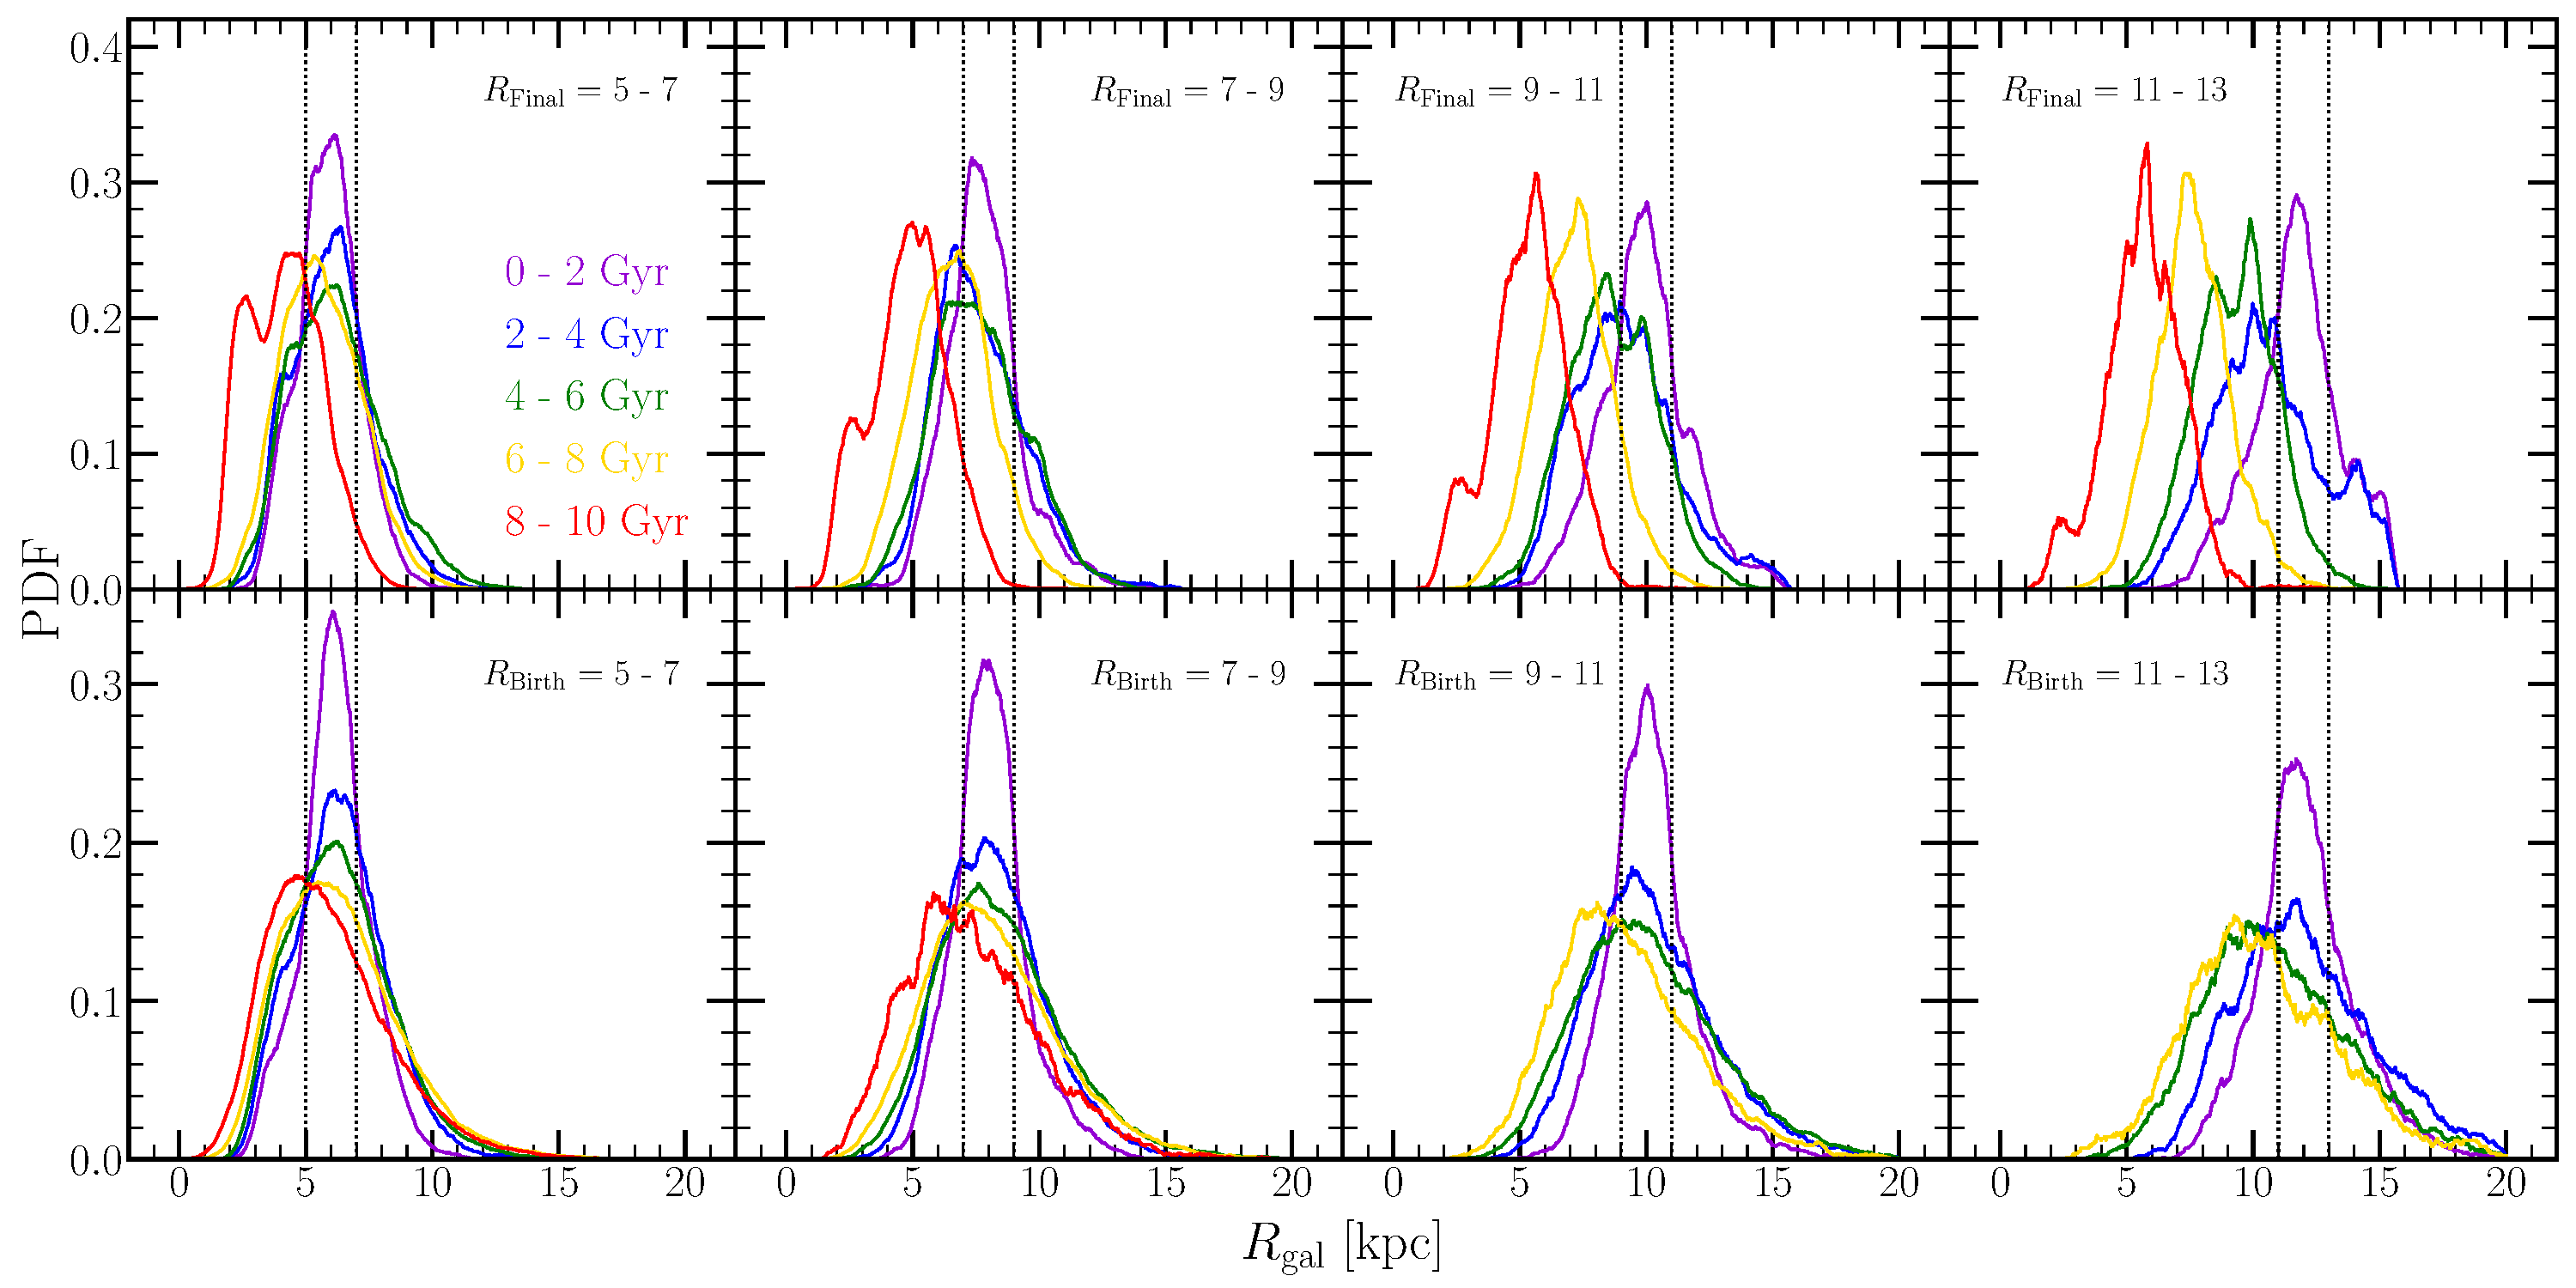
\includegraphics[scale = 0.32]{decomposition2.pdf} 
\caption{Radial distributions of our candidate analog star particles 
from~\texttt{h277}. In the top row, we show distributions of~\textit{birth} 
radius in bins of final radius and age. In the bottom row, we show 
distributions of~\textit{final} radius in bins of birth radius and age. Each 
bin in Galactocentric radius is shown in its own panel, denoted in text at the 
top the panels and by vertical black dashed lines. We color-code the 
distributions according to the age of the star particles and the legend in the 
upper left panel. We smooth all distributions with a box-car width of 0.5 kpc 
to improve clarity. We omit the distributions for 8 - 10 Gyr old stars born in 
the 9 - 11 and 11 - 13 kpc bins due to an insufficient number of star particles 
with which to calculate the distribution. }
\label{fig:h277_decomposition} 
\end{figure*} 

\begin{itemize} 
	\item In this paper we take~\texttt{h277}~\citep{Christensen2012, 
	Zolotov2012, Loebman2012, Loebman2014, Brooks2014}. Its data and our 
	migration schema are built directly into~\texttt{VICE}'s~\texttt{milkyway} 
	object as defaults for ease of use. A synopsis of the simulation parameters 
	can be found in~\S~2 of~\citet{Bird2020}. 

	\item Find that~\texttt{h277} has only a small fraction of star 
	particles born in the first 1 Gyr of its 13.7 Gyr run, so $T$ = 1 Gyr 
	is a much better estimate of the onset of star formation than 
	$T$ = 0 Gyr. Chop off the star particles born in the first Gyr of 
	evolution, and subtract 1 Gyr from their formation times, thus running 
	disk models for 12.7 Gyr. 

	\item Of particular importance to have accurately measured formation radii 
	for each star particle that we use as candidate analogs as discussed 
	in~\S~\ref{sec:methods:migration}.~\texttt{h277} did not record the 
	exact birth radius of each star particle; however, each star particle does 
	have an accurate age at each snapshot. Therefore, one has a reasonable 
	approximation of the birth radius of each star particle that is 
	sufficiently young in the first snapshot in which it was recorded. 
	Therefore, we restrict our sample of candidate analogs to those with an 
	age at first snapshot of~$\leq$ 150 Myr, and adopt their Galactocentric 
	radius at first snapshot as the birth radius. Also conducted the analysis 
	with age at first snapshot of~$\leq$50 Myr, and found similar results, 
	suggesting this choice does not impact our conclusions. In practice find 
	that 150 Myr also provides us with an adequately large number of star 
	particles to sample analogs from, such that our predicted abundance 
	distributions in various Galactic regions are not limited by stellar 
	population counts (in particular far off the plane). 

	\item Excluding halo stars, but including bulge, pseudobulge, and thin- 
	and thick-disk stars yields sample of 3,019,521 candidate analog star 
	particles. Included those because it's likely the majority formed within 
	a reasonably spatially confined region around the disk, suggesting they 
	contributed at least in part to its chemical evolution. 
	{\color{red} Expand on this: disk stars are only about 45\% of the total 
	sample, so our simulations run with~$\sim$1.5 million stellar populations 
	with assigned analogs to avoid oversampling. Plot distributions of 
	initial and final radii. } 

	\item Can be thought of as adopting the dynamical history of~\texttt{h277} 
	in our disk models. Advantage to this approach is that we get a migration 
	model with no free parameteres.~\citet{Minchev2013} adopts similar 
	approach with a hydrodynamical simulation, but did not investigate 
	time-dependent migration.~\citet{Schoenrich2009} did investigate 
	time-dependent migration, though their algorithm was based on dynamical 
	arguments rather than a hydrodynamical simulation, and required fitting 
	to observed data, for which they employed the Geneva-Copenhagen Survey of 
	solar neighbourhood stars~\citep{Nordstroem2004b, Holmberg2007}. We're 
	unaware of any studies to date which employ a hydrodynamical simulation 
	to drive radial migration while simultaneously allowing stars to 
	contribute to enrichment beyond their birth radius. 

	\item \texttt{h277} had a transient bar during its evolution, but does 
	not have a bar at $z$ = 0. This could mean that the star particles 
	in~\texttt{h277} migrated in a manner which does not reflect the dynamical 
	history of the Milky Way, but at present inferring a star's birth radius 
	observationally is notoriously difficult anyway ({\color{red} citation 
	needed}), so its likely the impact of this decision is within current 
	observational uncertainties. Nonetheless, it is worth noting that 
	the~\citet{Minchev2013} model, and by extension the~\citet{Minchev2014} 
	and~\citet{Minchev2017} models as well, selected a hydrodynamical 
	simulation specifically so that it would have a bar at $z$ = 0. A detailed 
	investigation of the impact of bar evolution on radial migration and thus 
	chemical evolution is outside the scope of this paper, though can be 
	conducted by simply swapping the birth times and initial and final radii 
	of~\texttt{h277} within~\texttt{VICE} and rerunning the simulations. 

	\item Distributions of birth radii in bins of final radii and age are 
	shown in the top row of Fig.~\ref{fig:h277_decomposition}. Conversely, the 
	bottom row shows distributions of final radii in bins of birth radii and 
	age. 
	\begin{itemize} 
		\item Focusing on the top row of panels in 
		Fig.~\ref{fig:h277_decomposition}, we note that the oldest stars at any 
		Galactocentric radius at the present day were overwhelmingly born at 
		smaller radii. The youngest stars, however, were overwhelmingly born at 
		that radius, and the stars of intermediate ages simply span the range 
		in radii between the two. With increasing radius, the differences in 
		the mode of the birth radius distribution between age bins gets larger. 

		\item Focusing on the bottom row of panels in 
		Fig.~\ref{fig:h277_decomposition}, we note that for stars born at any 
		radius and time, the distribution of final radii is still peaked near 
		the birth radius. With increasing age, it appears the mode final radius 
		may move slightly inward. The tails of the distributions to large radii 
		are relatively age-independent - some differences between the 0 - 2 and 
		8 - 10 Gyr age bins, but not much. However, the tails of the 
		distributions to small radii are not age-independent, and move toward 
		smaller $R_\text{gal}$ with increasing age. This suggests that radial 
		migration inward and outward occur on different timescales, in 
		particular that inward migration occurs on longer timescales than 
		outward migration. By extension this may suggest that inward and 
		outward migration are tied to different physical 
		processes.~\citet{Roskar2008a} demonstrate using a cosmological 
		simulation that resonant scattering at corotation causes stars to 
		move outward and gas to move inward. It's possible that radial 
		migration inward is has different origins. 

		\item The differences in distributions shown in the top and bottom 
		panels boils down to stellar surface density being a strong function 
		of Galactocentric radius. Take for example the age = 8 - 10 Gyr bin in 
		both $R_\text{Birth}$ = 5 - 7 kpc and $R_\text{Final}$ = 11 - 13 kpc 
		bins (i.e. the red curves in the bottom-left and top-right panels). 
		For these old stars born at 5 - 7 kpc, 11 - 13 kpc is far down the tail 
		of the $R_\text{Final}$ distribution, and yet 5 - 7 kpc is the mode 
		$R_\text{Birth}$ of all old stars presently at these radii. This is 
		only possible if the stellar surface density gradient is sufficiently 
		steep, which it is known to be~\citep[e.g.][]{Bland-Hawthorn2016}. 
		\begin{itemize} 
			\item Fig.~\ref{fig:h277_decomposition} also demonstrates that the 
			numbers of stars that migrated inward and outward are comparable 
			in~\texttt{h277}. Taking a~$\left|\Delta R_\text{gal}\right| \geq$ 
			500 pc between birth and final radii as the criterion for migrating 
			inward or outward, indeed we find that in our sample of candidate 
			analogs, 27\% migrated inward, 29\% migrated outward, and the 
			remaining 44\% stayed near their birth radius. 
		\end{itemize} 

		\item In all bins of birth radius, a good first-order estimate of the 
		probability density that a star has a final radius in the same bin 
		is~$\sim$0.2 - 0.3. With bins in radius on this plot of 2 kpc, that 
		suggests that 40 - 60\% of stars migrate significantly beyond their 
		birth radius by the time they're~$\sim$2 Gyr old. If the SN Ia DTD is a 
		$t^{-1.1}$ power-law as suggested by recent 
		observations~\citep[e.g.][]{Maoz2012, Maoz2017}, then we expect similar 
		numbers of SN Ia events to occur with delay times between 1 and 10 Gyr 
		as we do between 100 Myr and 1 Gyr. With such an extended DTD, and the 
		distributions in final radius shown in the bottom panel of 
		Fig.~\ref{fig:h277_decomposition}, its possible that white dwarfs 
		migrate significant distances before producing a SN Ia event. This is 
		the motivation for our test of whether or not the radial migration of 
		nucleosynthetic yields is a statistically significant effect. 
	\end{itemize} 
\end{itemize} 


\subsection{Nucleosynthetic Yields} 
\label{sec:methods:yields} 
\begin{itemize} 
	\item Brief background on~\texttt{VICE}'s algorithm: we form a given 
	number of stellar populations in each zone and at each timestep. They 
	then migrate between zones according to our algorithm and eject CCSN and 
	SN Ia products as smooth functions of time according to our yields. 

	\item \textit{Fractional net} yields, as required by~\texttt{VICE}. 

	\item Take our yields from~\citet{Weinberg2017} and~\citet{Johnson2020}. 
	Find that our models with these yields predict [O/Fe] $\approx$ +0.05 for 
	zero age stars, so we multiply SN Ia Fe yield by $10^{0.1}$ to produce 
	more realistic late-time [O/Fe]. This is likely within the uncertainties 
	in nucleosynthetic yields. 

	\item CCSN products injected immediately, and thus unaffected by 
	migration: 
	\begin{equation} 
	\dot{M}_x^\text{CC} = y_x^\text{CC}\dot{M}_\star 
	\end{equation} 

	\item SN Ia products injected with a $t^{-1.1}$ DTD, with minimum delay 
	$t_\text{D}$ = 150 Myr. 
	\begin{equation} 
	\dot{M}_x^\text{Ia} = y_x^\text{Ia} \sum_i M_i R_\text{Ia}(\tau_i) 
	\end{equation} 
	where the summation is taken over all stellar populations in a given zone, 
	and $M_i$ and $\tau_i$ denote the mass and age of the $i$'th stellar 
	population in a given zone at a given time. The SN Ia rate $R_\text{Ia}$ 
	is normalized such that the integral over the time interval from 
	$t_\text{D}$ to a maximum time of 15 Gyr is equal to one. 

	\item We include AGB star enrichment according to the FRUITY database net 
	yields~\citep{Cristallo2011}, though these yields are not significant 
	compared to the CCSN and SN Ia yields for O and Fe. Our results can be 
	interpreted as if they were zero. Algorithm is based on 
	calculating the mass in dying stars from previously formed stellar 
	populations at each timestep, details can be found in~\citet{Johnson2020} 
	and in~\texttt{VICE}'s science documentation\footnote{
		\url{https://vice-astro.readthedocs.io/en/latest/science_documentation/enrichment/index.html} 
	}. 

	\item \citet{Minchev2013} adopt much lower nucleosynthetic yields, 
	because they don't have outflows. Discuss differences in how we obtain the 
	late-time metallicity gradient either here or at the end 
	of~\S~\ref{sec:methods:outflows}. 
\end{itemize} 

\subsection{Outflows} 
\label{sec:methods:outflows} 

\begin{figure} 
\centering 
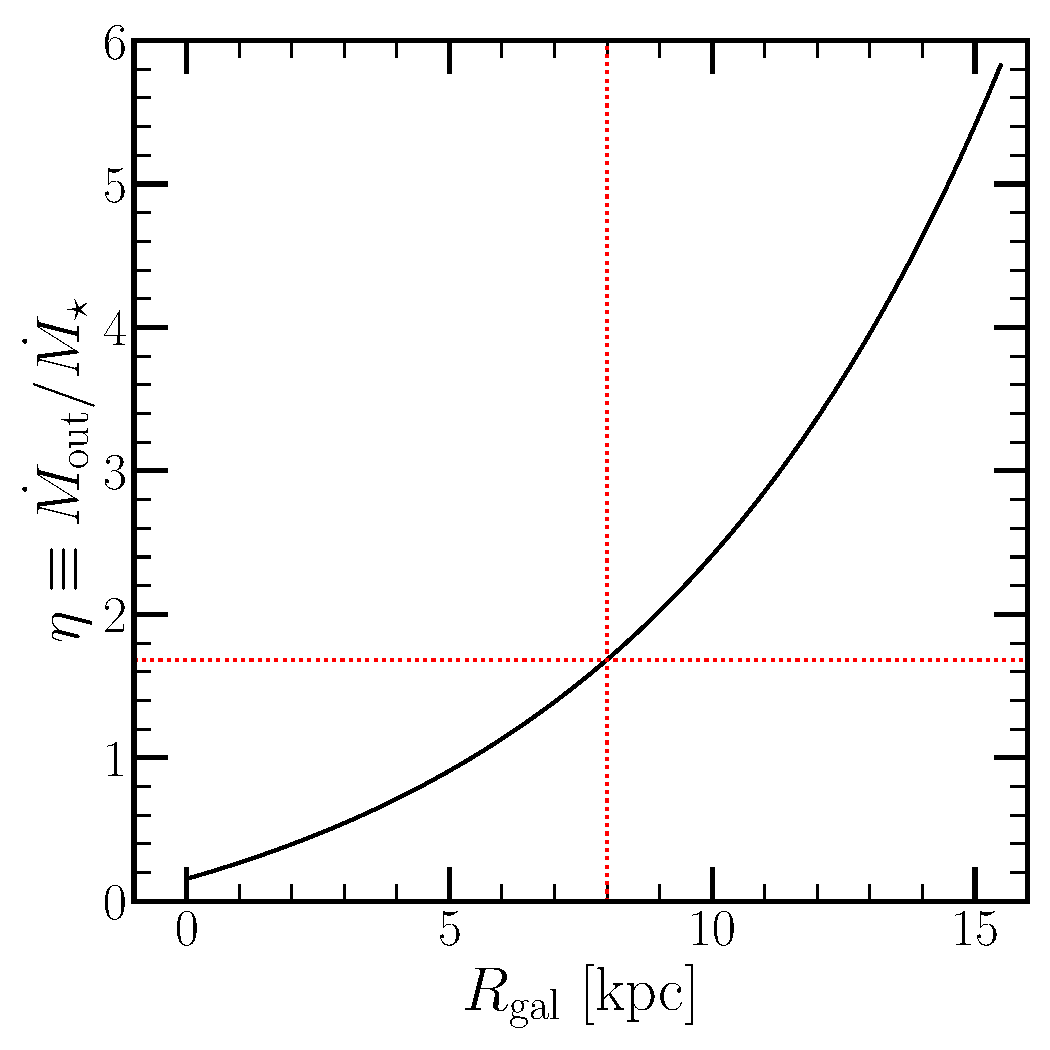
\includegraphics[scale = 0.45]{eta.pdf} 
\caption{Our implemented scaling of the mass loading factor $\eta$ with 
Galactocentric radius (black) as defined by equation~\refp{eq:eta}. The 
horizontal and vertial red dashed lines highlight the value of $\eta \approx$ 
1.7 at an assumed orbital radius of the sun of $R_\odot$ = 8 kpc. } 
\label{fig:eta} 
\end{figure} 

\begin{itemize} 
	\item $\eta \equiv \dot{M}_\text{out}/\dot{M}_\star$ 

	\item Implement a scaling of $\eta$ with $R_\text{gal}$ such that a 
	realistic metallicity gradient is produced at late times. A fundamental 
	observable, the observed metallicity gradient in the Milky Way has been the 
	focus of a considerable number of studies to date. 
	\begin{itemize} 
		\item \citet{Nordstroem2004a} find a gradient of -0.099 kpc$^{-1}$ in 
		[Fe/H] in main sequence stars from GCS~\citep{Nordstroem2004b, 
		Holmberg2007}. 

		\item \citet{Daflon2009} find a gradient of -0.04 kpc$^{-1}$ in 
		[S/H] in OB stars 

		\item \citet{Frinchaboy2013} find a gradient of -0.09 kpc$^{-1}$ in 
		[M/H] in open clusters. 

		\item \citet{Hayden2014} also find -0.09 kpc$^{-1}$ in [M/H] for 
		$R_\text{gal}\gtrsim$ 6 kpc for low-$\alpha$ stars. For 
		$R_\text{gal}\lesssim$ 6 kpc, they find a relatively flat gradient. 

		\item \citet{Weinberg2019} finds -0.06 kpc$^{-1}$ in mode([Mg/H]) for 
		upper red giant branch disk stars (see their Fig. 23). 
	\end{itemize} 

	\item The procedure outlined in this section reproduces the metallicity 
	gradient while neglecting the impact of radial migration. We demonstrate 
	in~\S~\ref{sec:gradients:metallicity} that this assumption holds in our 
	simulation outputs which do take it into account. 

	\item Our recipe for ensuring a reasonable gradient hinges on the 
	assumption that the mode [X/H] for any given element $x$ at any given 
	radius $R_\text{gal}$ reflects the equilibrium abundance of that element at 
	that radius. 

	\item For $\alpha$ elements,~\citet{Weinberg2017} defines the equilibrium 
	abundance under a constant SFH as: 
	\begin{equation} 
	Z_{\alpha,\text{eq}} = \frac{y_\alpha^\text{CC}}{1 + \eta(R_\text{gal}) - r} 
	\end{equation} 
	where $\eta$ is the mass-loading factor at that radius $R_\text{gal}$, and 
	$r$ is the recycling parameter ($\approx$ 0.4 for the sake of this 
	scaling with a~\citetalias{Kroupa2001} IMF;~\citealp{Weinberg2017}). 
	Solving for $\eta(R_\text{gal})$ yields: 
	\begin{equation} 
	\eta(R_\text{gal}) = \frac{y_\alpha^\text{CC}}{Z_{\alpha,\text{eq}}} + r - 1 
	= \frac{y_\alpha^\text{CC}}{Z_{\alpha,\odot}}10^{-\text{mode([X/H])}
	(R_\text{gal})} + r - 1 
	\end{equation} 

	\item We assume a slope of -0.08 kpc$^{-1}$, in tentative agreement with 
	the previous studies that quote the slope of the gradient mentioned above. 
	To set the normalization, we assume the mode([X/H]) to be~$\sim$+0.3 at 
	$R_\text{gal}$ = 4 kpc, since this would produce mode([X/H])~$\approx$~0 at 
	$R_\text{gal}\approx$ 7 - 9 kpc. This results in the following form for 
	$\eta$ as a function of Galactocentric radius: 
	\begin{equation} 
	\eta(R_\text{gal}) = \frac{y_\alpha^\text{CC}}{Z_{\alpha,\odot}} 
	10^{(-0.08\text{ kpc}^{-1})(R_\text{gal} - \text{4 kpc}) + 0.3} + r - 1 
	\label{eq:eta} 
	\end{equation} 

	\item This does assume a uniformly linear gradient at all $R_\text{gal}$. 
	\citet{Hayden2014} do find the gradient in [M/H] to flatten for 
	$R_\text{gal}\lesssim$ 6 kpc, challenging this assumption. However, this 
	procedure can be easily repeated for any desired gradient, since the 
	functional form simply goes into the power of 10 in equation~\refp{eq:eta}. 

	\item Model based on assumption that observed mode([$\alpha$/H]) as a 
	function of Galactocentric radius reflects the equilibrium $\alpha$ 
	abundance at each radius (i.e. mode([$\alpha$/H]) = 
	$\log_{10}(Z_{\alpha,\text{eq}}/Z_{\alpha,\odot})$)

	\item We adopt our yield of O for $y_\alpha^\text{CC}$ and the solar 
	abundance of O of $Z_{\text{O},\odot}$ = 0.00572 from~\citet{Asplund2009}. 

	\item Fig.~\ref{fig:eta} plots this scaling of~$\eta$ with~$R_\text{gal}$, 
	highlighting the value for the solar circle. 

	\item \citet{Minchev2013} did not include outflows in their model, and as 
	such have much lower yields. Discuss differences in how we obtain the 
	late-time metallicity gradient either here or at the end 
	of~\S~\ref{sec:methods:yields}. 
\end{itemize} 

\subsection{Recycling} 
\label{sec:methods:recycling} 
\begin{itemize} 
	\item As mentioned in~\S~\ref{sec:methods:yields}, we're using~\textit{net} 
	rather than~\textit{gross} yields. Our yields thus only quantify the amount 
	of~\textit{newly produced} metals from each stellar population, and the 
	return of previously produced material must be taken into account. 

	\item \citet{Weinberg2017} defined the~\textit{cumulative return fraction}
	$r$ to be the fraction of a single stellar population's initial mass that 
	has been returned to the ISM. In detail, $r$ is a complicated function of 
	the age of a stellar population $\tau$ which depends on the assumptions 
	about stellar lifetimes, the IMF, and an initial-remnant mass 
	relation~\citep[e.g.][]{Kalirai2008}. 
	\begin{itemize} 
		\item \citet{Weinberg2017} demonstrated that the assumption 
		of~\textit{instantaneous recycling} is a reasonable approximation, 
		where instantaneous recycling refers only to previously produced 
		material, contrary to what most people mean when the refer to 
		instantaneous recycling. They show that $r$ = 0.4 (0.2) is a good 
		approximation for a~\citetalias{Kroupa2001} (\citetalias{Salpeter1955}) 
		IMF. However, this was demonstrated for smooth star formation histories 
		and in parameter spaces conducive to analytic solution. Because 
		numerical integration of $r(\tau)$ is neither challenging nor 
		time-consuming,~\texttt{VICE} by default implements continuous recycling 
		by solving $r(\tau)$ at the beginning of each simulation given the 
		IMF, the~\citet{Kalirai2008} initial-remnant mass model, and the 
		assumption that $\tau = \tau_\odot(M/M_\odot)^{-3.5}$. We also assume 
		a post-main sequence lifetime of 10\% of the main sequence lifetime for 
		all stars. 
	\end{itemize} 

	\item The detailed form the recycling rate in a given annulus and at a 
	given time is: 
	\begin{equation} 
	\dot{M}_x^\text{r} = \sum_i Z_{x,i} M_i \dot{r}(\tau_i) 
	\end{equation} 
	where $M_i$ is the mass of the $i$'th stellar population in the annulus, 
	$\tau_i$ is its age, $Z_{x,i}$ is its birth abundance of some element $x$, 
	and the summation is taken over all stellar populations in the annulus at 
	that time. 

	\item We implement continuous recycling in our simulations, but at a number 
	of places in analyzing their results here, we adopt the instantaneous 
	approximation for ease. 
\end{itemize} 

\subsection{Star Formation Histories} 
\label{sec:methods:sfhs} 

\begin{figure} 
\centering 
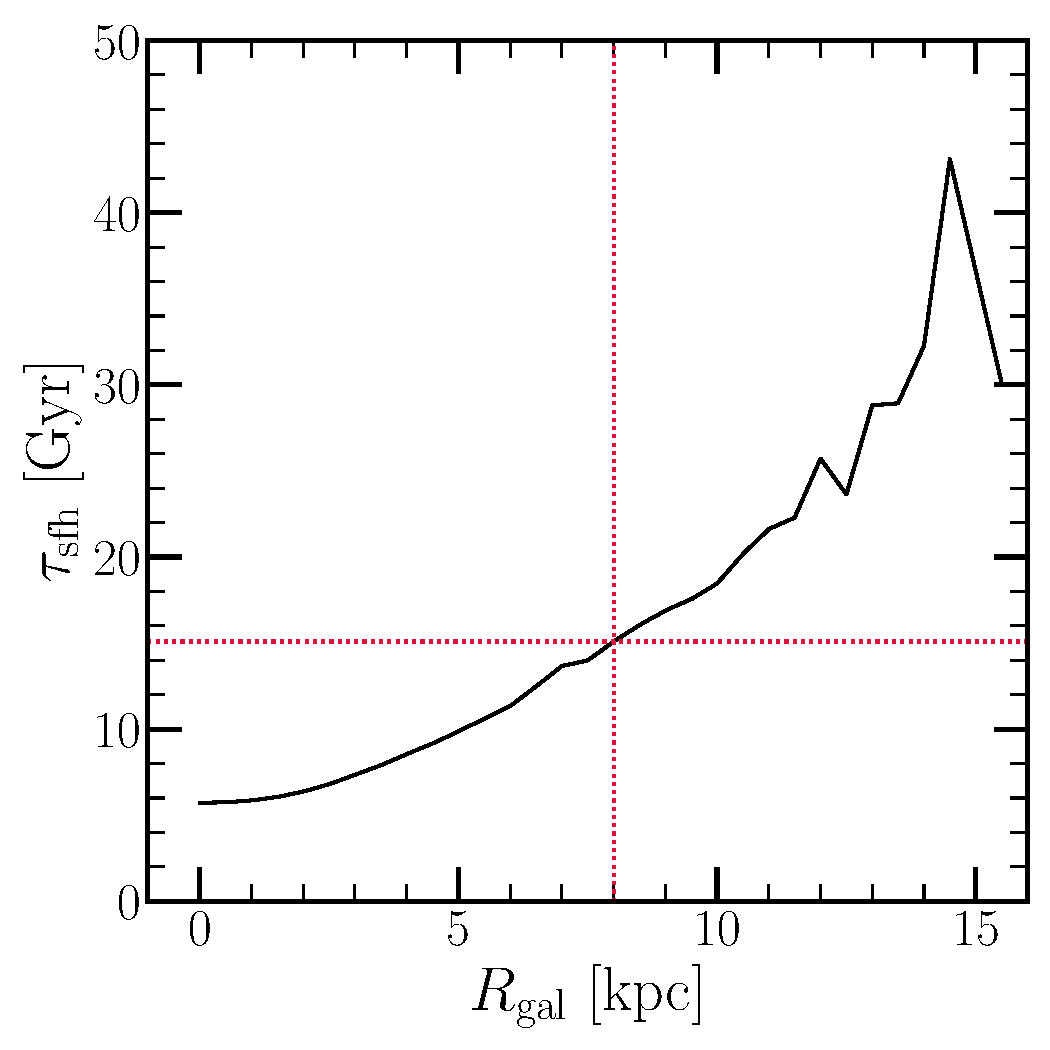
\includegraphics[scale = 0.45]{tau_sfh.pdf} 
\caption{The e-folding timescales of star formation as reported 
by~\citet{Sanchez2020} for $10^{10.5}$ - $10^{11}$ M$_\odot$ Sa/Sb Hubble type 
galaxies (black), assuming a half-light radius of $R_\text{e}$ = 5 kpc and the 
mathematical form of our inside-out SFH (see equation~\refp{eq:insideout_sfh}). 
The red dotted lines highlight $\tau_\text{sfh}~\approx$ 15 Gyr at an assumed 
radius of the sun of $R_\odot$ = 8 kpc. }
\label{fig:tau_sfh}
\end{figure} 

\begin{figure*} 
\centering 
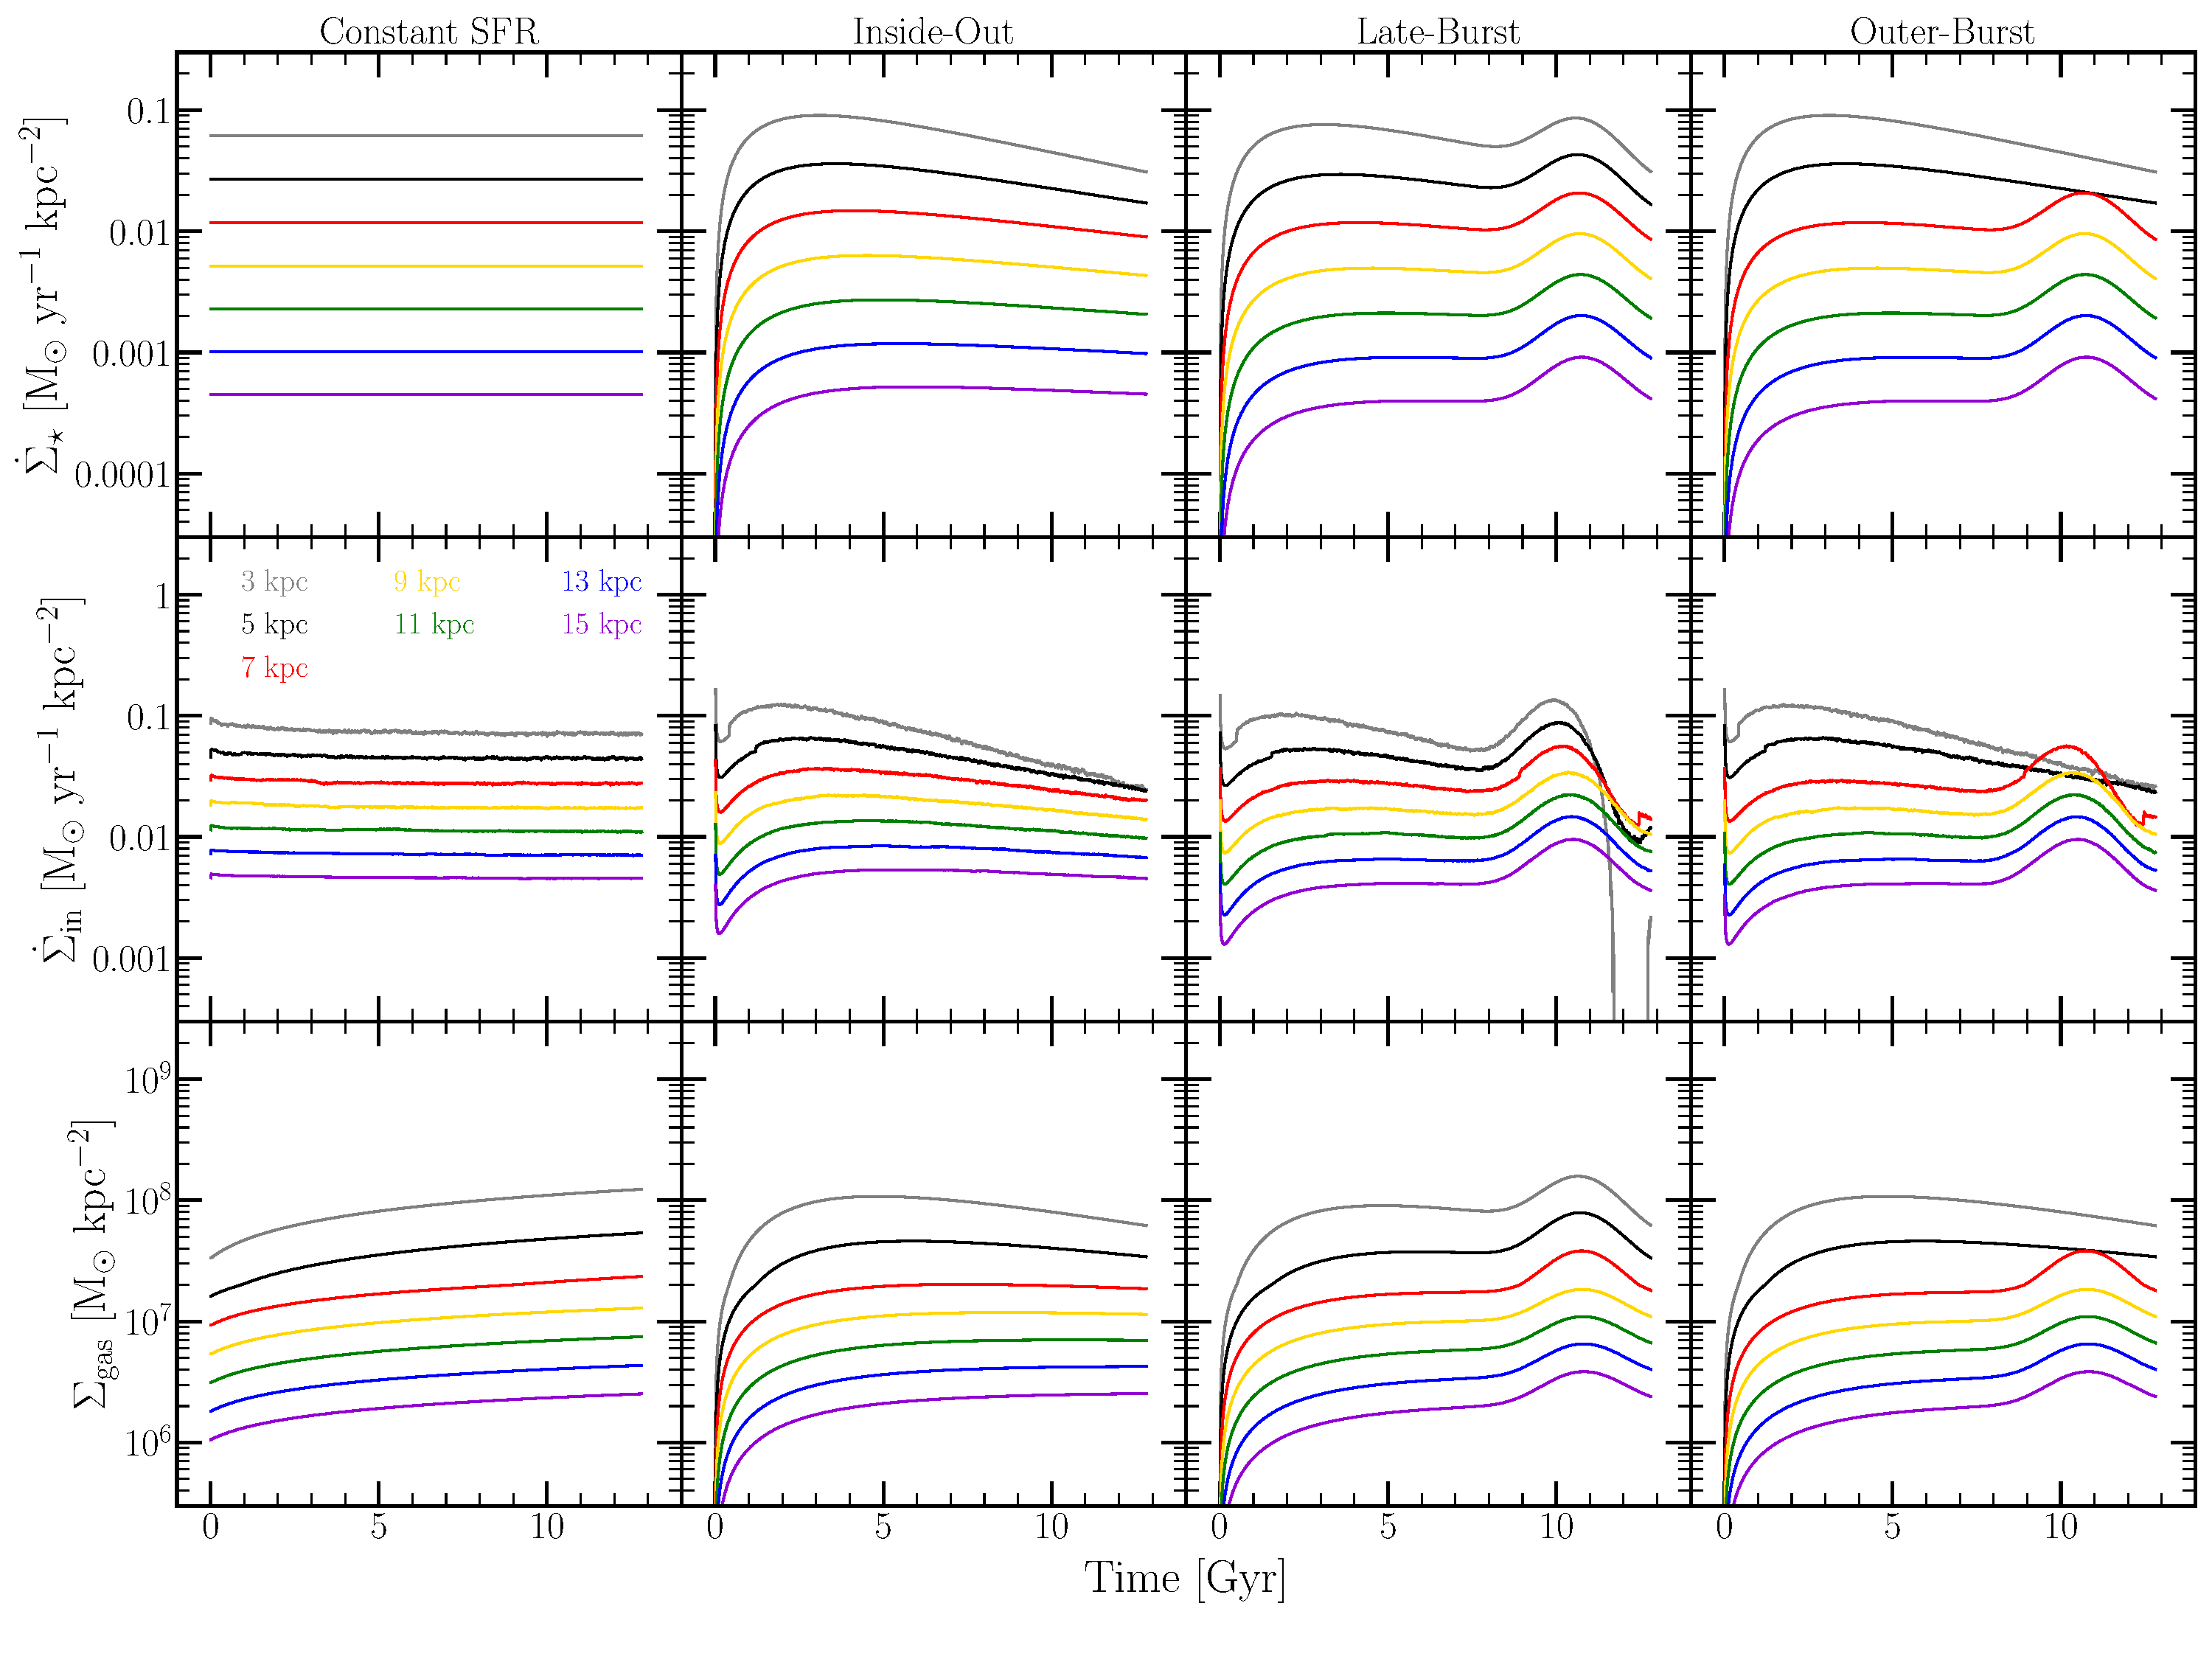
\includegraphics[scale = 0.32]{sfh.pdf} 
\caption{The surface densities of star formation $\dot{\Sigma}_\star$ (top 
row), infall $\dot{\Sigma}_\text{in}$ (middle row), and gas $\Sigma_\text{gas}$ 
(bottom row) as functions of simulation time for our four fiducial SFHs: 
constant (far left), inside-out (left middle), late-burst (right-middle), 
and outer-burst (far right). We plot curves for the annuli whose inner radii 
are 3 kpc (grey), 5 kpc (black), 7 kpc (red), 9 kpc (yellow), 11 kpc (green), 
13 kpc (blue), and 15 kpc (purple) (see equations~\refp{eq:constant_sfh}, 
\refp{eq:insideout_sfh},~\refp{eq:lateburst_sfh}, and~\refp{eq:outerburst_sfh} 
for the mathematical definition of each SFH). } 
\label{fig:evol} 
\end{figure*} 

\begin{itemize} 
	\item Appendix~\ref{sec:normalize_sfh} presents justification of how we 
	normalize our parameters to produce a realistic Milky Way at the end of 
	the simulation. In short, it takes in a unitless description of the 
	time-dependence of the SFH at a given Galactocentric radius, denoted 
	$f(t|R_\text{gal})$, and a unitless description of the radial dependence of 
	the present-day stellar surface density, denoted $g(R_\text{gal})$. 
	Neglecting radial migration, it then integrates $f(t|R_\text{gal})$ at each 
	radius with time and $g(R_\text{gal})$ over the area of the disk to ensure 
	that the correct present-day stellar mass and desired surface density 
	gradient $\Sigma_\star$ are produced by the simulation. This recipe hinges 
	on the assumption that radial migration does not significantly alter the 
	form of $\Sigma_\star$, which we demonstrate 
	in~\S~\ref{sec:gradients:density} to be the case under our model and 
	for~\texttt{h277}'s dynamical history. As long as this assumption isn't 
	violated, this recipe can be used. 

	\item Adopt the~\citet{Licquia2015} total stellar mass of 
	$(6.08\pm1.14)\times10^{10}~M_\odot$. We're including bulge star particles 
	in our sample of candidate analogs from~\texttt{h277}, so we model the 
	entire stellar mass as opposed to just the disk, for 
	which~\citet{Licquia2015} found $(5.17\pm1.11)\times10^{10}~M_\odot$. 

	\item Take the gradient from~\citet{Bland-Hawthorn2016}, which characterize 
	the disk as a double exponential - the sum of two single exponentials 
	representing the thin and thick disks. This has the following form: 
	\begin{equation} 
	g(R_\text{gal}) = e^{-R_\text{gal}/r_\text{t}} + 
	\frac{\Sigma_\text{T}}{\Sigma_\text{t}}e^{-R_\text{gal}/R_\text{T}} 
	\end{equation} 
	where $r_\text{t}$ and $r_\text{T}$ are the scale radii of the thin and 
	thick disks, respectively, and $\Sigma_\text{T}/\Sigma_\text{t}$ is the 
	ratio of the surface densities to thin and thick disk stars at 
	$R_\text{gal}$ = 0. Based on the results of~\citet{Bland-Hawthorn2016}, we 
	take in this paper $r_\text{t}$ = 2.5 kpc, $r_\text{T}$ = 2.0 kpc, and 
	$\Sigma_\text{T}/\Sigma_\text{t}$ = 0.27. 

	\item We present four fiducial SFHs, which we dub ``constant'', 
	``inside-out'', ``late-burst'', and ``outer-burst''. They're defined as 
	follows: 
	\begin{itemize} 
		\item \textbf{Constant}: The SFH at a given radius is time-independent. 
		\begin{equation} 
		f_\text{C}(t|R_\text{gal}) = 1 
		\label{eq:constant_sfh} 
		\end{equation} 
		This case is of particular theoretical interest because it quantifies 
		the effect of ongoing with star formation with radial migration, and 
		no additional effects. 

		\item \textbf{Inside-Out}: 
		\begin{equation} 
		f_\text{IO}(t|R_\text{gal}) = (1 - e^{-t/\tau_\text{rise}})
		e^{-t/\tau_\text{sfh}} 
		\label{eq:insideout_sfh} 
		\end{equation} 
		We adopt this scenario over the traditional linear-times-exponential 
		form of $f(t|R_\text{gal})~\sim~te^{-t/\tau_\text{sfh}}$, because the 
		latter does not offer control over the position of the maximum. The 
		form we adopt has a maximum near $\tau_\text{rise}$, for which we adopt 
		a value 2 Gyr everywhere in this paper. We find that this produces a 
		peak in star formation at lookback times of~$\sim$10 Gyr, corresponding 
		to a redshift of~$z \approx$~2, which is around cosmic high noon. In 
		this paper $\tau_\text{sfh}$ is a function of $R_\text{gal}$ here, and 
		we discuss it briefly in a few paragraphs. 

		\item \textbf{Late-Burst}: An inside-out SFH with a gaussian describing 
		a starburst. 
		\begin{equation} 
		f_\text{LB}(t|R_\text{gal}) = f_\text{IO}(t|R_\text{gal}) 
		(1 + A_\text{b}e^{-(t - t_\text{b})^2/2\sigma_\text{b}^2}) 
		\label{eq:lateburst_sfh} 
		\end{equation} 
		$A_\text{b}$ is a dimensionless parameter describing the strength of 
		the starburst, $t_\text{b}$ is the time of the local maximum in the SFH 
		during the burst, and $\sigma_\text{b}$ is the width of the gaussian 
		describing it. Loosely motivated by the findings of~\citet{Isern2019} 
		and~\citet{Mor2019}. Here we take $A_\text{b}$ = 1.5, $t_\text{b}$ = 
		10.8 Gyr, and $\sigma_\text{b}$ = 1 Gyr. 

		\item \textbf{Outer-Burst}: A variation of the late-burst model in 
		which only $R_\text{gal}\geq$ 6 kpc experience the starburst. Loosely 
		motivated by findings of~\citet{Vincenzo2020} where a hydrodynamical 
		simulation of a Milky Way-like galaxy showed radially dependent 
		infall. 
		\begin{equation} 
		f_\text{OB}(t|R_\text{gal}) = \begin{cases} 
		f_\text{IO}(t|R_\text{gal}) & (R_\text{gal}~<~\text{6 kpc}) \\ 
		f_\text{LB}(t|R_\text{gal}) & (R_\text{gal}~\geq~\text{6 kpc}) 
		\end{cases} 
		\label{eq:outerburst_sfh} 
		\end{equation} 
	\end{itemize} 

	\item Derive e-folding timescales of star formation $\tau_\text{sfh}$ 
	from the data in~\citet{Sanchez2020}. 
	\begin{itemize} 
		\item They present the stellar surface density $\Sigma_\star$ as a 
		function of age in bins of $R/R_\text{e}$ for MaNGA galaxies, where 
		$R_\text{e}$ is the half-light radius. They conduct this analysis in 
		bins of stellar mass and for different Hubble types. Here take their 
		M$_\star$ = 10$^{10.5}$ - 10$^{11}$ M$_\odot$ bin for Sa/Sb spirals 
		(i.e. Milky Way-like galaxies). 

		\item With our gradient, we know the present-day half-mass radius to be 
		very near 4 kpc (this is just doing a couple integrals over the area of 
		the disk). The findings of~\citet{Garcia-Benito2017} and 
		\citet{GonzalezDelgado2014} suggest that half-light radii are 
		marginally larger than half-mass radii. Based on equations (4) of 
		\citet{GonzalezDelgado2014} relation the two for circular apertures, 
		we expect our model galaxy to have a half-light radius near 5 kpc. We 
		therefore adopt $R_\text{e}$ = 5 kpc in calculating $\tau_\text{sfh}$ 
		as a function of radius. {\color{red} As I understand it, there are 
		some results that suggest this value for the Milky Way as well?} 

		\item Their reported $\Sigma_\star$-age relation is not robust enough 
		to get individual SFHs directly, but does allow the parameters of some 
		fiducial mathematical model to be fit to the population-averaged data. 
		Assuming the $f_\text{IO}(t|R_\text{gal})$ form, we simultaneously fit 
		the normalization and the e-folding timescale $\tau_\text{sfh}$ to 
		these data. Although the normalization is irrelevant to our simulations 
		and determined via the method outlined in 
		Appendix~\ref{sec:normalize_sfh}, we adopt the resulting 
		$\tau_\text{sfh}$-$R_\text{gal}$ relation in our models. Results are 
		shown in Fig.~\ref{fig:tau_sfh}. 

		\item Note that the star formation timescales are long, even for the 
		solar annulus ($\tau_\text{sfh} \approx$~15 Gyr at $R_\odot$ = 8 kpc) 
		and especially for the outer galaxy. Beyond the solar annulus, SFHs are 
		nearly constant after the initial rise at early times. 
	\end{itemize} 

	\item Given the assumed star formation histories, the gas supply at all 
	times is known via the SFE timescale $\tau_\star$ (discussed 
	in~\S~\ref{sec:methods:sfe}). With the amount of gas lost to star formation 
	and outflows at each timestep, the infall rate is also known at all 
	timesteps. The results of all three are shown in Fig.~\ref{fig:evol}. 
\end{itemize} 

\subsection{Star Formation Efficiency} 
\label{sec:methods:sfe} 

\begin{figure*} 
\centering 
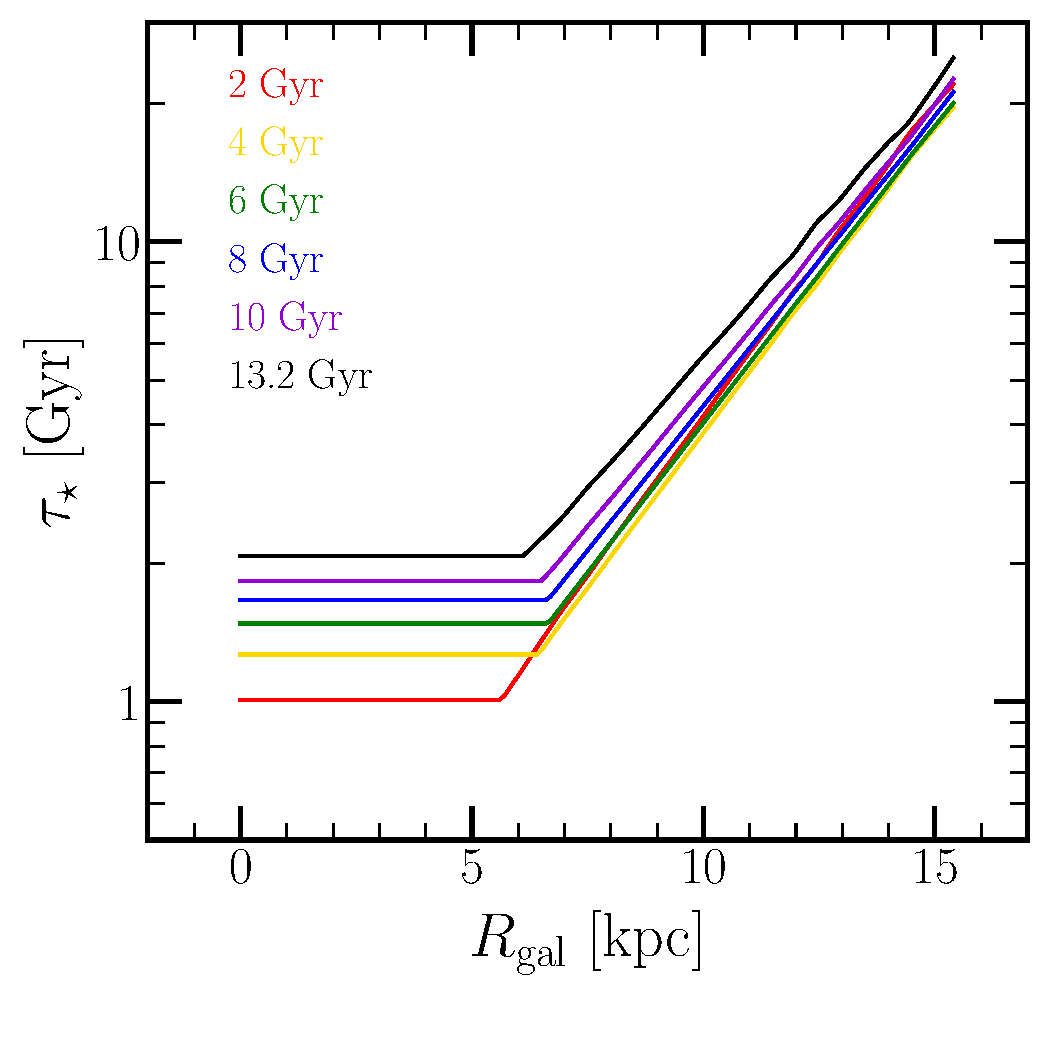
\includegraphics[scale = 0.32]{sfe.pdf} 
\caption{The star formation efficiency (SFE) timescale $\tau_\star$ as a 
function of Galactocentric radius at simulation times of 2 Gyr (red), 4 Gyr 
(yellow), 6 Gyr (green), 8 Gyr (blue), 10 Gyr (purple), and 12.7 Gyr (i.e. 
the present day, black) for our four fiducial SFHs: constant (left), inside-out 
(left-middle), late-burst (right-middle), and outer-burst (right). }
\label{fig:sfe} 
\end{figure*} 

\begin{itemize} 
	\item The term ``star formation efficiency'' (SFE) is an overloaded term in 
	the literature. In the star formation/ISM literature, it usually refers to 
	the fraction of a molecular cloud's mass which will eventually be converted 
	into stars. In the chemical evolution literature, however, it usually 
	refers to the inverse timescale relating the star formation rate within 
	some gas reservoir and the mass of the gas reservoir itself: 
	$\tau_\star \equiv M_\text{gas}/\dot{M}_\star$. High (Low) values of 
	$\tau_\star$ indicate slow (fast) star formation and thus low (high) SFE; 
	when we refer to SFE here, we're referring to the definition based on this 
	timescale. 
	\begin{itemize} 
		\item Potentially note that this is often referred to as the 
		``depletion time'' in the ISM literature, and the~\citet{Weinberg2017} 
		definition of depletion 
		time:~$\tau_\text{dep} \equiv \tau_\star/ (1 + \eta - r)$. 

		\item In our models, $\tau_\star$ increases with decreasing molecular 
		fraction: $\tau_\star = \tau_\star^\text{mol}/f_\text{mol}$, where 
		$\tau_\star^\text{mol}$ is the same parameter, but for gas that is 
		entirely H$_2$. We let it bottom out at this value because it's 
		believed that star formation proceeds in the molecular phase, although 
		there is significant scatter in the observed relation~\citep[e.g.][]{
		Leroy2008, Kennicutt2012, Tacconi2018}. 
	\end{itemize} 

	\item Here we implement a modified Kennicutt-Schmidt Law~\citep{Schmidt1959, 
	Schmidt1963, Kennicutt1998} to describe the scaling of~$\tau_\star$ 
	with~$\Sigma_g$. Below some threshold density $\Sigma_{g,\text{Crit}}$, we 
	adopt a power-law with index $k$ = 0.5, based on the $N$ = 1.5 power-law 
	describing the~$\dot{\Sigma}_\star-\Sigma_g$ relation\footnote{
		$k = N - 1$~\citep{Johnson2020}. 
	}. Above this threshold, we assume the molecular fraction in the ISM to be 
	unity, and to form stars at the rate determined by $\tau_\star^\text{mol}$. 
	That is: 
	\begin{equation} 
	\tau_\star = \begin{cases} 
	\tau_\star^\text{mol}\left(\frac{\Sigma_g}{\Sigma_{g,\text{Crit}}}\right)^k 
	& (\Sigma_g \leq \Sigma_{g,\text{Crit}}) \\ 
	\tau_\star^\text{mol} & (\Sigma_g \geq \Sigma_{g,\text{Crit}}) 
	\end{cases} 
	\end{equation} 
	It's common in the chemical evolution literature to adopt a pure power-law 
	scaling of~$\tau_\star$ with~$\Sigma_g$; we adopt this alternate form with 
	a minimum value to ensure that the implied $\tau_\star$ is never below 
	$\tau_\star^\text{mol}$ at any redshift. 

	\item Observationally,~$\Sigma_{g,\text{Crit}}$ is the surface density at 
	which the observed Kennicutt-Schmidt relation switches from quadratic to 
	linear.~\citet{Bigiel2008} present observed Kennicutt-Schmidt relations 
	from the HERACLES and BIMA surveys, and~\citet{Krumholz2018} presents a 
	compilation of Kennicutt-Schmidt relations observed by~\citet{Bigiel2010} 
	and~\citet{Leroy2013}. Both suggest that the value is at or around 
	$\sim10$~M$_\odot$~pc$^{-2}$ = $10^7$~M$_\odot$~kpc$^{-2}$. 
	{\color{red} In practice we find that this predicts a seemingly 
	unrealistically high ISM composition - $f_\text{mol}$ = 1 for 
	$R_\text{gal}\lesssim$ 6 kpc, so in this outline we've ran our simulations 
	with $\Sigma_{g,\text{Crit}} = 2\times10^7$~M$_\odot$~kpc$^{-2}$. 
	However, this did not solve the problem. We're still debating about what 
	prescription to use here, though the choice makes no difference in our 
	models. It's likely the final version of this paper will make a simple 
	assumption regarding star formation efficiency, and then demonstrate in 
	Appendix~\ref{sec:sfe_variations} that the impact is not significant. }

	% \item {\color{red} The following is not yet in this outline. The models 
	% included here are with $\Sigma_{g,\text{Crit}} = 2\times10^7$~M$_\odot$ 
	% kpc$^{-2}$. This value predicts a global $f_\text{mol}$ = 84\%, which is 
	% much higher than observations. In a subsequent version, there will be an 
	% appendix demonstrating the value of $\Sigma_{g,\text{Crit}}$ that predicts 
	% $f_\text{mol} \approx$~0.35. Based on my current estimates, it's somewhere 
	% around~$\sim5\times10^8$ M$_\odot$ kpc$^{-2}$. We've looked at models with 
	% $\Sigma_{g,\text{Crit}} = 10^8$~M$_\odot$~kpc$^{-2}$, and found similar 
	% conclusions, so we don't expect this parameter to have an impact, but we 
	% want to be presenting the most realistic galaxy in the main body of the 
	% paper. The appendix will likely also demonstrate that these variations are 
	% not impactful. }

	\item \citet{Tacconi2018} suggest that~$\tau_\star^\text{mol}$ should 
	scale with redshift~$z$ and the deviation from the star forming main 
	sequence~$\delta\text{MS}$ via~$\tau_\star^\text{mol} \propto (1 + z)^{-0.6} 
	\delta\text{MS}^{-0.44}$. We don't take into account the effect of 
	$\delta\text{MS}$ in our models, but we do investigate the redshift 
	dependence. A reasonable approximation to the $t-z$ relation out 
	to~$z \approx$~3 is: 
	\begin{equation} 
	\frac{t}{t_0} \approx (1 + z)^{-5/4} 
	\end{equation} 
	where $t_0$ is the present-day age of the universe, and $t$ is not 
	simulation time but the age of the universe at any given redshift. 
	Plugging this relation into the~\citet{Tacconi2018} scaling yields the 
	following time-dependence for~$\tau_\star^\text{mol}$: 
	\begin{equation} 
	\tau_\star^\text{mol} = \tau_{\star,0}^\text{mol}(t/t_0)^{12/25} \approx 
	\tau_{\star,0}^\text{mol}(t/t_0)^{1/2} 
	\end{equation} 
	where $\tau_{\star,0}^\text{mol}$ is simply $\tau_\star^\text{mol}$ at the 
	present day. We generalize this formula to the following form: 
	\begin{equation} 
	\tau_\star^\text{mol} = \tau_{\star,0}^\text{mol}(t/t_0)^\beta 
	\end{equation} 
	In this paper we present simulations which adopt~$\tau_{\star,0}^\text{mol}$ 
	= 2 Gyr and~$\beta$~= 1/2. We have however ran all possible combinations of 
	$\tau_{\star,0}^\text{mol}$ = 1 and 2 Gyr,~$\beta$~= 0 and 1/2, all four 
	of our fiducial SFHs, and all four migration models, a total of 64 
	simulations. Unless otherwise noted, we find similar results in all 
	dimensions except SFH. 

	\item Fig.~\ref{fig:sfe} shows $\tau_\star$ as a function of $R_\text{gal}$ 
	at six different time stamps predicted by our fiducial models. 
	Wherever~$\tau_\star$ is at its minimum value is where the ISM is fully 
	molecular. 
	\begin{itemize} 
		\item From the actual value of $\tau_\star$ at a given radius and time 
		and the assumed $\tau_\star^\text{mol}$ in the model, we can derive 
		molecular fractions within the disk. In the models present here, 
		the disk is molecular out to~$R_\text{gal} \approx$~6 kpc in all models 
		at the present day. The inside-out SFH has a global molecular fraction 
		of~$f_\text{mol} \approx$~84\%. 
	\end{itemize} 
\end{itemize} 

\subsection{Simulation Parameters} 
\label{sec:methods:simparams} 

\begin{itemize} 
	\item \texttt{VICE}'s simulations runs in either infall, star formation, or 
	gas mode, referring simply to which one the user is specifying. The 
	fiducial starburst models presented in~\citet{Johnson2020} ran in infall 
	mode, but here we run things in star formation mode, since we are after 
	specific forms for the star formation histories of our models. 

	\item We have a sample of 3,019,521 candidate analog star particles 
	from~\texttt{h277}, only~$\sim$57\% of which are disk stars. Since we're 
	modeling the thin and thick disk populations here,~$\sim$1.72 million is a 
	much better estimate of the number of analogs that we can realistically 
	sample from. We let star formation extend out to 15.5 kpc, beyond which 
	we force the star formation rate to zero at all times.~\texttt{VICE} does 
	form stellar populations at all timesteps in the annuli; they simply have 
	zero mass and thus do not contribute to the chemical evolution or recycling, 
	though they contribute to the computational overhead. With 200 zones and 
	1,271 timesteps, we let~\texttt{VICE} form~$n$ = 8 stellar populations per 
	zone per timestep, resulting in 2,033,600 stellar populations with 
	predicted masses and abundances, 1,565,872 of which form 
	between~$R_\text{gal}$ = 0 and 15.5 kpc, reasonably within the limit of 
	what we can sample. These simulations run in~$\sim$2 hours and take 
	up~$\sim$235 MB per output, including the extra data that we record for 
	each stellar population's analog star particle. 
	\begin{itemize} 
		\item To ensure that resolution does not affect our results, we ran the 
		same set of models with~$n$ = 2 stellar populations per zone per 
		timestep, and found similar predictions. 
	\end{itemize} 
\end{itemize} 

\subsection{The Observed Sample} 
\label{sec:methods:observed_sample} 

\begin{itemize} 
	\item For the age-metallicity and age-[$\alpha$/Fe] relations, we compare 
	to the results of~\citet{Feuillet2019}. Also compared 
	to~\citet{Feuillet2018}, the primary difference being that solar 
	metallicity stars are found to be considerably younger in the earlier 
	study. 

	\item {\color{red} I pulled some of this information from David's 
	two-process paper, which used DR14. Let me know if any of the details of 
	APOGEE and the data reduction have changed since then. }
	Compare metallicity distribution functions to the 16th data release 
	(DR16;~\citealp{Ahumada2020}) of the Apache Point Observatory Galaxy 
	Evolution Experiment (APOGEE;~\citealp{Majewski2017}). A part of the Sloan 
	Digital Sky Survey (SDSS), APOGEE data is collected with a 300-fiber 
	H-band spectrograph~\citep{Wilson2020} on the 2.5-meter Sloan Foundation 
	telescope at Apache Point Observatory~\citep{Gunn2006}. The APOGEE sample 
	largely consists of evolved stars with 2MASS~\citep{Skrutskie2006} 
	magnitudes in the range 7 < $H$ < 13.8 sampled on a grid of sightlines 
	at Galactic latitudes $b$ = -8$^\circ$, -4$^\circ$, 0$^\circ$, +4$^\circ$, 
	and +8$^\circ$ and a wide range of longitudes. \citet{Nidever2015} 
	describes the data processing pipeline for APOGEE, providing the input to 
	the APOGEE Stellar Parameters and Chemical Abundances Pipeline (ASPCAP; 
	\citealp{Holtzman2015,GarciaPerez2016}). ASPCAP simultaneously fits 
	elemental abundances, effective temperatures, and surface gravities using a 
	grid of synthetic spectra predicted by 1-dimensional stellar atmospheric 
	models assuming local thermodynamic equilibrium~\citep{Meszaros2012, 
	Zamora2015} and the spectral line list provided in~\citep{Shetrone2015}. 
	{\color{red} (1-D LTE correct?)} 

	\item While we make use of DR16 in comparing our predicted MDFs to the 
	APOGEE data,~\citet{Feuillet2018} and~\citet{Feuillet2019} made use of the 
	14th data release (DR14;~\citealp{Abolfathi2014}). We don't expect this 
	slight difference to impact our conclusions. 
\end{itemize} 


\section{Gradients} 
\label{sec:gradients} 

\begin{figure} 
\centering 
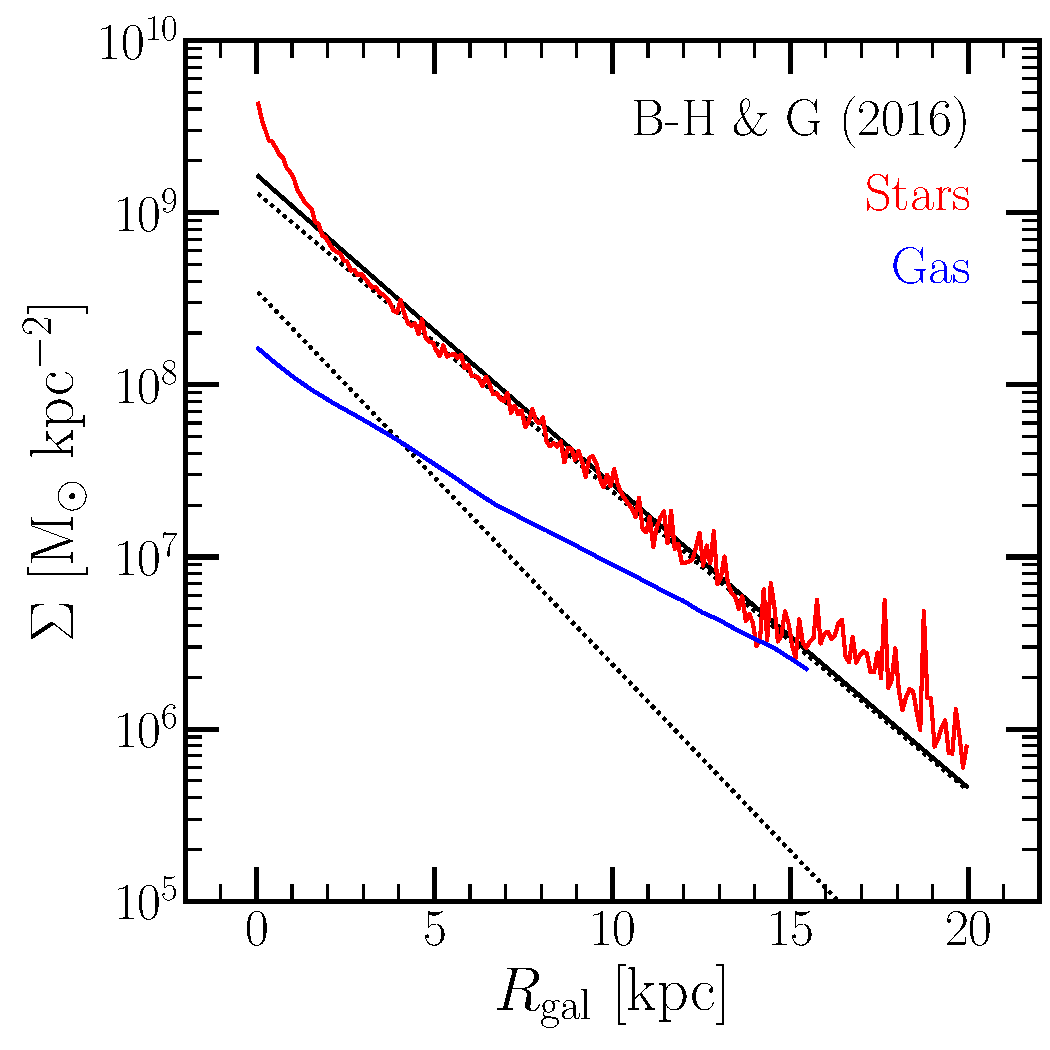
\includegraphics[scale = 0.45]{surface_density_gradient_timedep.pdf} 
\caption{The surface density of gas (blue) and stars (red) as predicted by our 
model with an inside-out SFH, diffusion migration, and 
$\tau_\star^\text{mol} = (\text{2 Gyr})(t/t_0)^{1/2}$. The dotted black lines 
denote the exponential fit to the thin- and thick-disk profiles reported 
by~\citet{Bland-Hawthorn2016}, with the black solid line denoting the sum of 
the two, all renormalized to imply the same total stellar mass within the 
disk. }
\label{fig:surface_density} 
\end{figure} 

\begin{figure*} 
\centering 
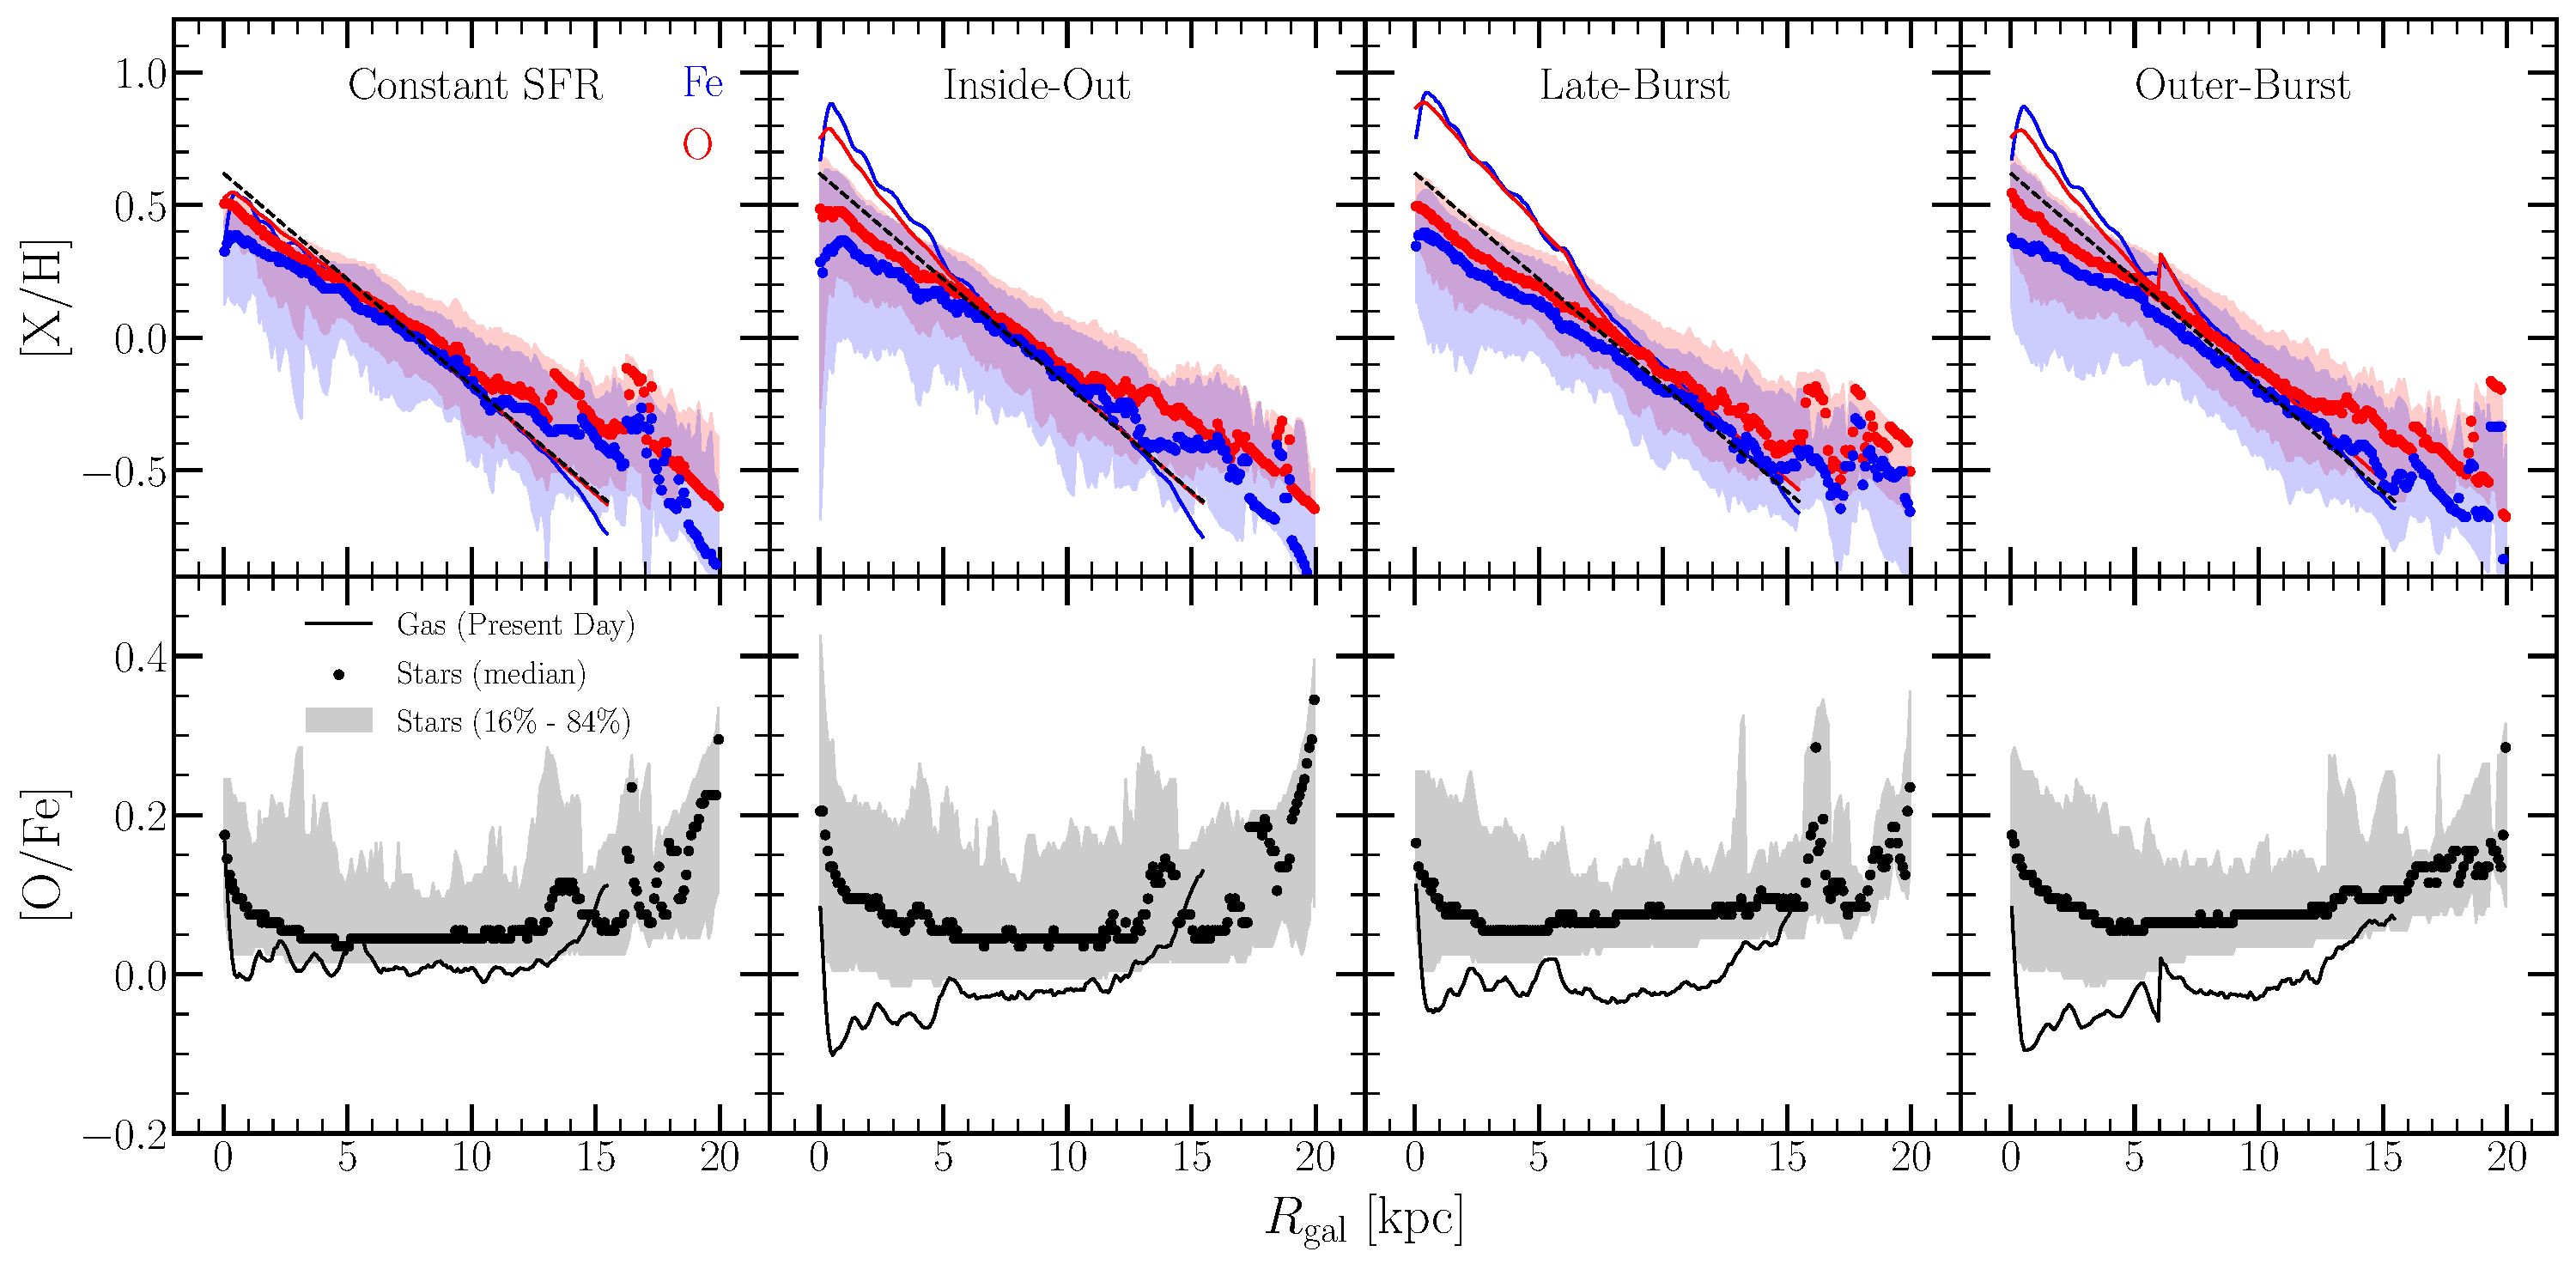
\includegraphics[scale = 0.32]{metallicity_gradient.pdf} 
\caption{Radial abundance gradients in [O/H] (top, red) [Fe/H] (top, blue), 
and [O/Fe] (bottom) for our four fiducial SFHs - constant (far left), 
inside-out (left-middle), late-burst (right-middle), and outer-burst (far 
right). We plot the gas phase abundance at the present day as a function of 
Galactocentric radius in solid lines. Stars denote the mode of the stellar 
MDF of the 100-pc width annulus at a given radius, with shaded regions 
marking the 16th and 84th percentiles thereof. Black lines in the top panels 
denote our target [$\alpha$/H] gradient of mode([$\alpha$/H]) = +0.3 at 
$R_\text{gal}$ = 4 kpc with a slope of -0.06 kpc$^{-1}$. } 
\label{fig:metallicity_gradient} 
\end{figure*} 

\subsection{Surface Density} 
\label{sec:gradients:density} 

\begin{itemize} 
	\item SFH in each annulus normalized such that, neglecting radial 
	migration, a given gradient is reproduced (see 
	Appendix.~\ref{sec:normalize_sfh}). Here we've adopted a double 
	exponential with scale radii $r_\text{t}$ = 2.5 kpc, $r_\text{T}$ = 2.0 
	kpc, and $\Sigma_\text{T}/\Sigma_\text{t}$ = 0.27 at $R_\text{gal}$ = 
	0~\citep{Bland-Hawthorn2016}. Both are plotted as dotted black lines in 
	Fig.~\ref{fig:surface_density}, and the sum as a solid black line. 

	\item Surface density gradient from model with inside-out SFH, diffusion 
	migration, and $\tau_\star^\text{mol} = (\text{2 Gyr})(t/t_0)^{1/2}$ 
	plotted in Fig.~\ref{fig:surface_density} as well (stars in red and gas 
	in blue). Radial migration indeed didn't change the overall scaling of 
	$\Sigma_\star$ with $R_\text{gal}$ at the radii that we care about in 
	this paper ($\gtrsim$3 kpc), only introducing scatter. Gas disk appears to 
	be well-fit by a single-exponential with scale radius of~$\sim$3-4 kpc. 

	\item Increase in~$\Sigma_\star$ at~$R_\text{gal} \lesssim$ 2 kpc likely 
	due to stellar populations finding bulge or pseudobulge star particles as 
	analogs and migrating inward. {\color{red} Comment further on this, and 
	plot PDFs of the kinematically decomposed star particles 
	from~\texttt{h277}: essentially zero bulge and pseudobulge star particles 
	with either birth or final radii~$\gtrsim$ 3 kpc.} 
\end{itemize} 

\subsection{Metallicity} 
\label{sec:gradients:metallicity} 

\begin{itemize} 
	\item Scaling of $\eta$ with $R_\text{gal}$ based on reproducing the 
	observed mode([$\alpha$/H])-$R_\text{gal}$ trend, neglecting radial 
	migration (see~\S~\ref{sec:methods:outflows}). The target gradient is 
	shown in a solid black line in Fig.~\ref{fig:metallicity_gradient}. 

	\item Gradient is indeed recovered in [O/H], and radial migration appears 
	to only induce scatter. While Fe did not enter into our procedure for 
	setting the metallicity gradient, the model predicts a similar gradient 
	for [Fe/H]. 

	\item Metal-poor and $\alpha$-enhanced tail in the inner galaxy predicted 
	by all models. 

	\item Details of the [O/Fe] gradient seem to be sensitive to differences 
	in our SFHs. 

	\item Constant SFH is the only model in which the present-day gas phase 
	gradient matches the stellar gradient at all radii. In remaining models, 
	the present-day gas-phase abundance is above the majority of the stars 
	because the star formation rate has decreased. 

	\item Stellar gradient is somewhat shallower in the late-burst model; this 
	is because of the dilution associated with the starburst. Target gradient 
	represents the equilibrium abundance at all radii, and we deliberately 
	perturbed it from equilibrium, so any deviations from the expectation are 
	a consequence of that. 

	\item Late-burst model has super-equilibrium gas phase abundance at the 
	present day. Can be seen in the break in the gas phase gradient in the 
	outer-burst as well. This is a consequence of the starburst - in infall 
	driven starbursts, re-enrichment can produce super-equilibrium abundances 
	which then decay back to the equilibrium abundance as the star 
	formation rate declines~\citep{Johnson2020}. 
\end{itemize} 

\section{Metallicity Space} 
\label{sec:metallicity_space} 

\begin{figure*} 
\centering 
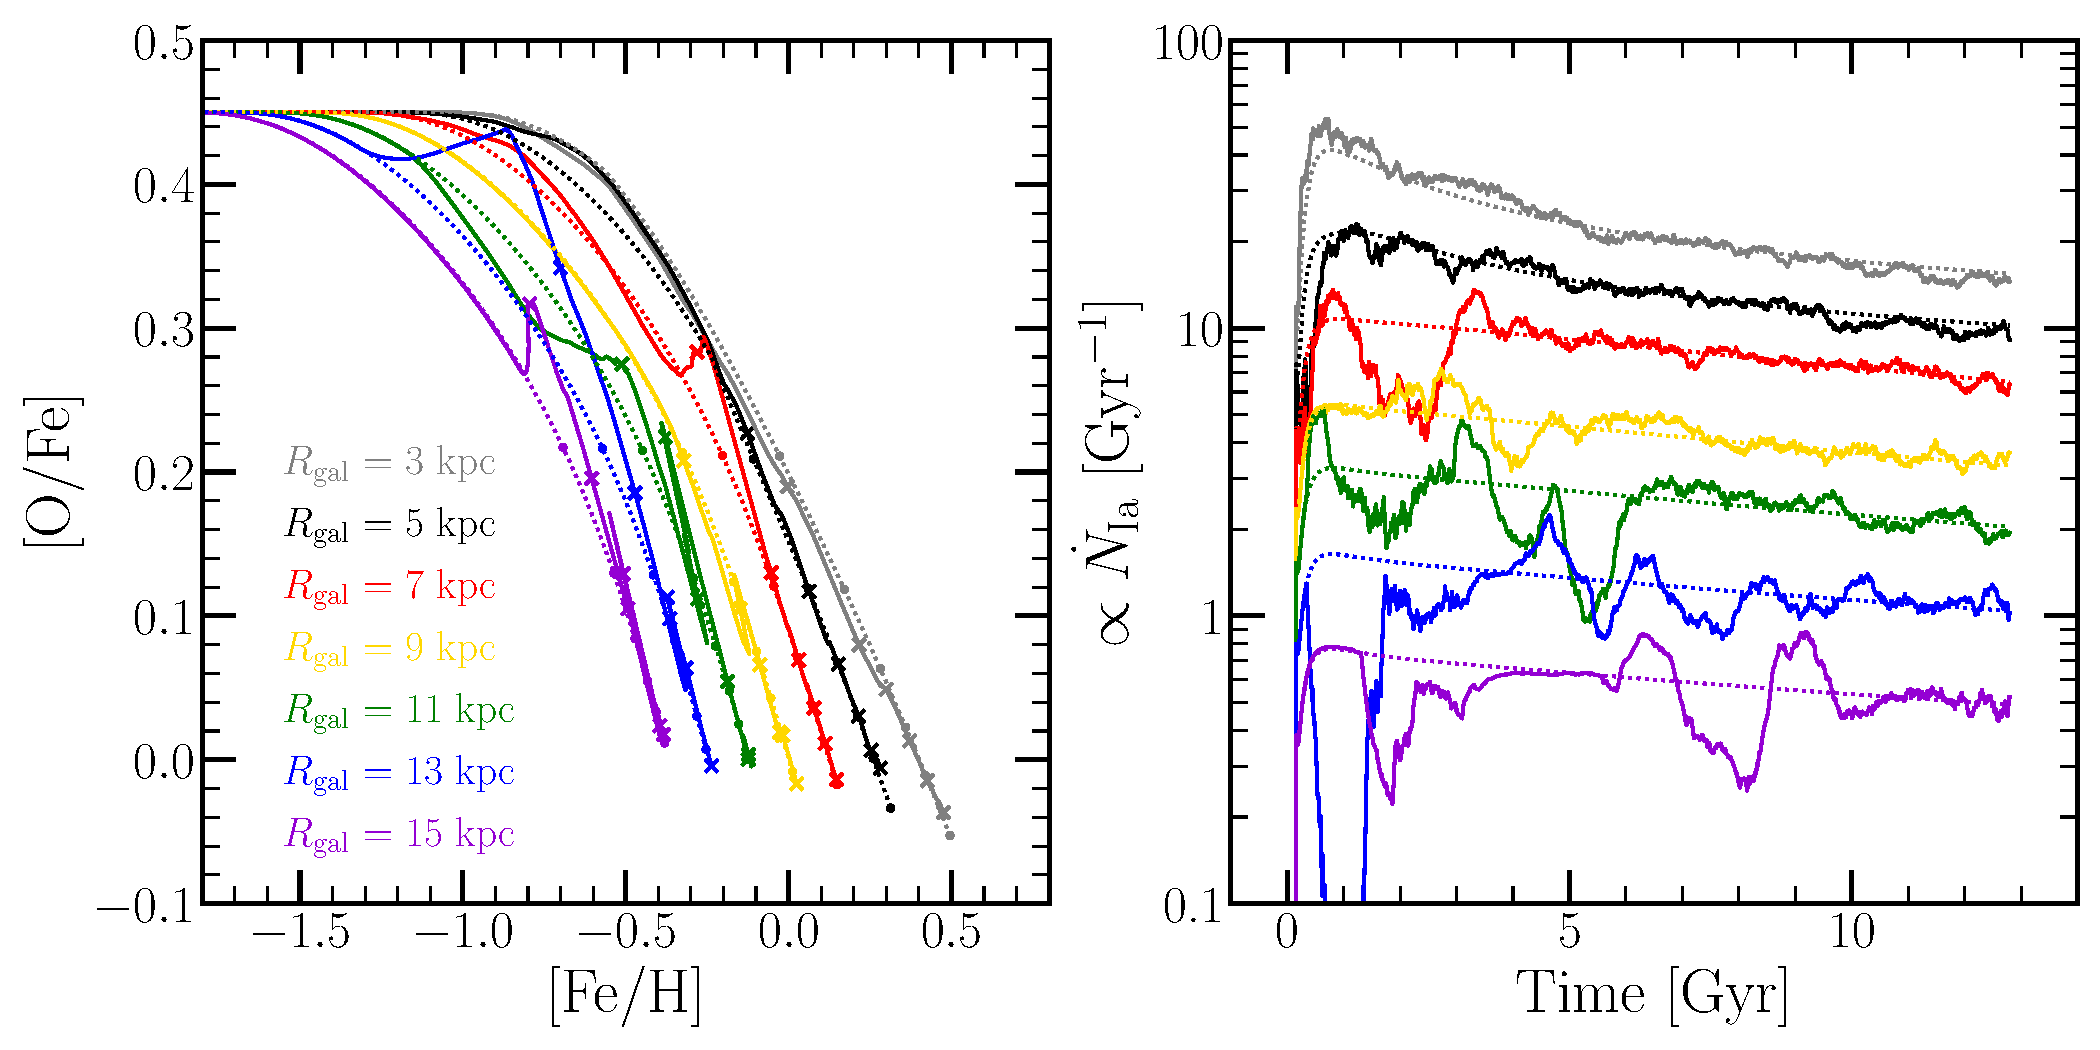
\includegraphics[scale = 0.42]{tracks_2Gyr_timedep.pdf} 
\caption{\textbf{Left}: Evolutionary tracks for the gas phase in the 
[O/Fe]-[Fe/H] plane for models with 
$\tau_\star^\text{mol} = (\text{2 Gyr})(t/t_0)^{1/2}$, our inside-out SFH, and 
either post-processing (dotted lines) or diffusion (solid lines) migration 
models. We plot tracks for seven annuli, color-coded according to their 
Galactocentric radius and denoted by the legend in the lower-left. We mark 
simulation times of 2, 4, 6, 8, 10, and 12.7 Gyr in X's for the diffusion 
model and points for the post-processing model. 
\textbf{Right}: The proxy for the SN Ia rate defined in equation 
\refp{eq:ia_rate_proxy} as a function of simulation time for the same annuli 
as in the left-hand panel. We multiply rates at each radii here by various 
prefactors in the interest of clarity. }
\label{fig:tracks} 
\end{figure*} 

\begin{figure*} 
\centering 
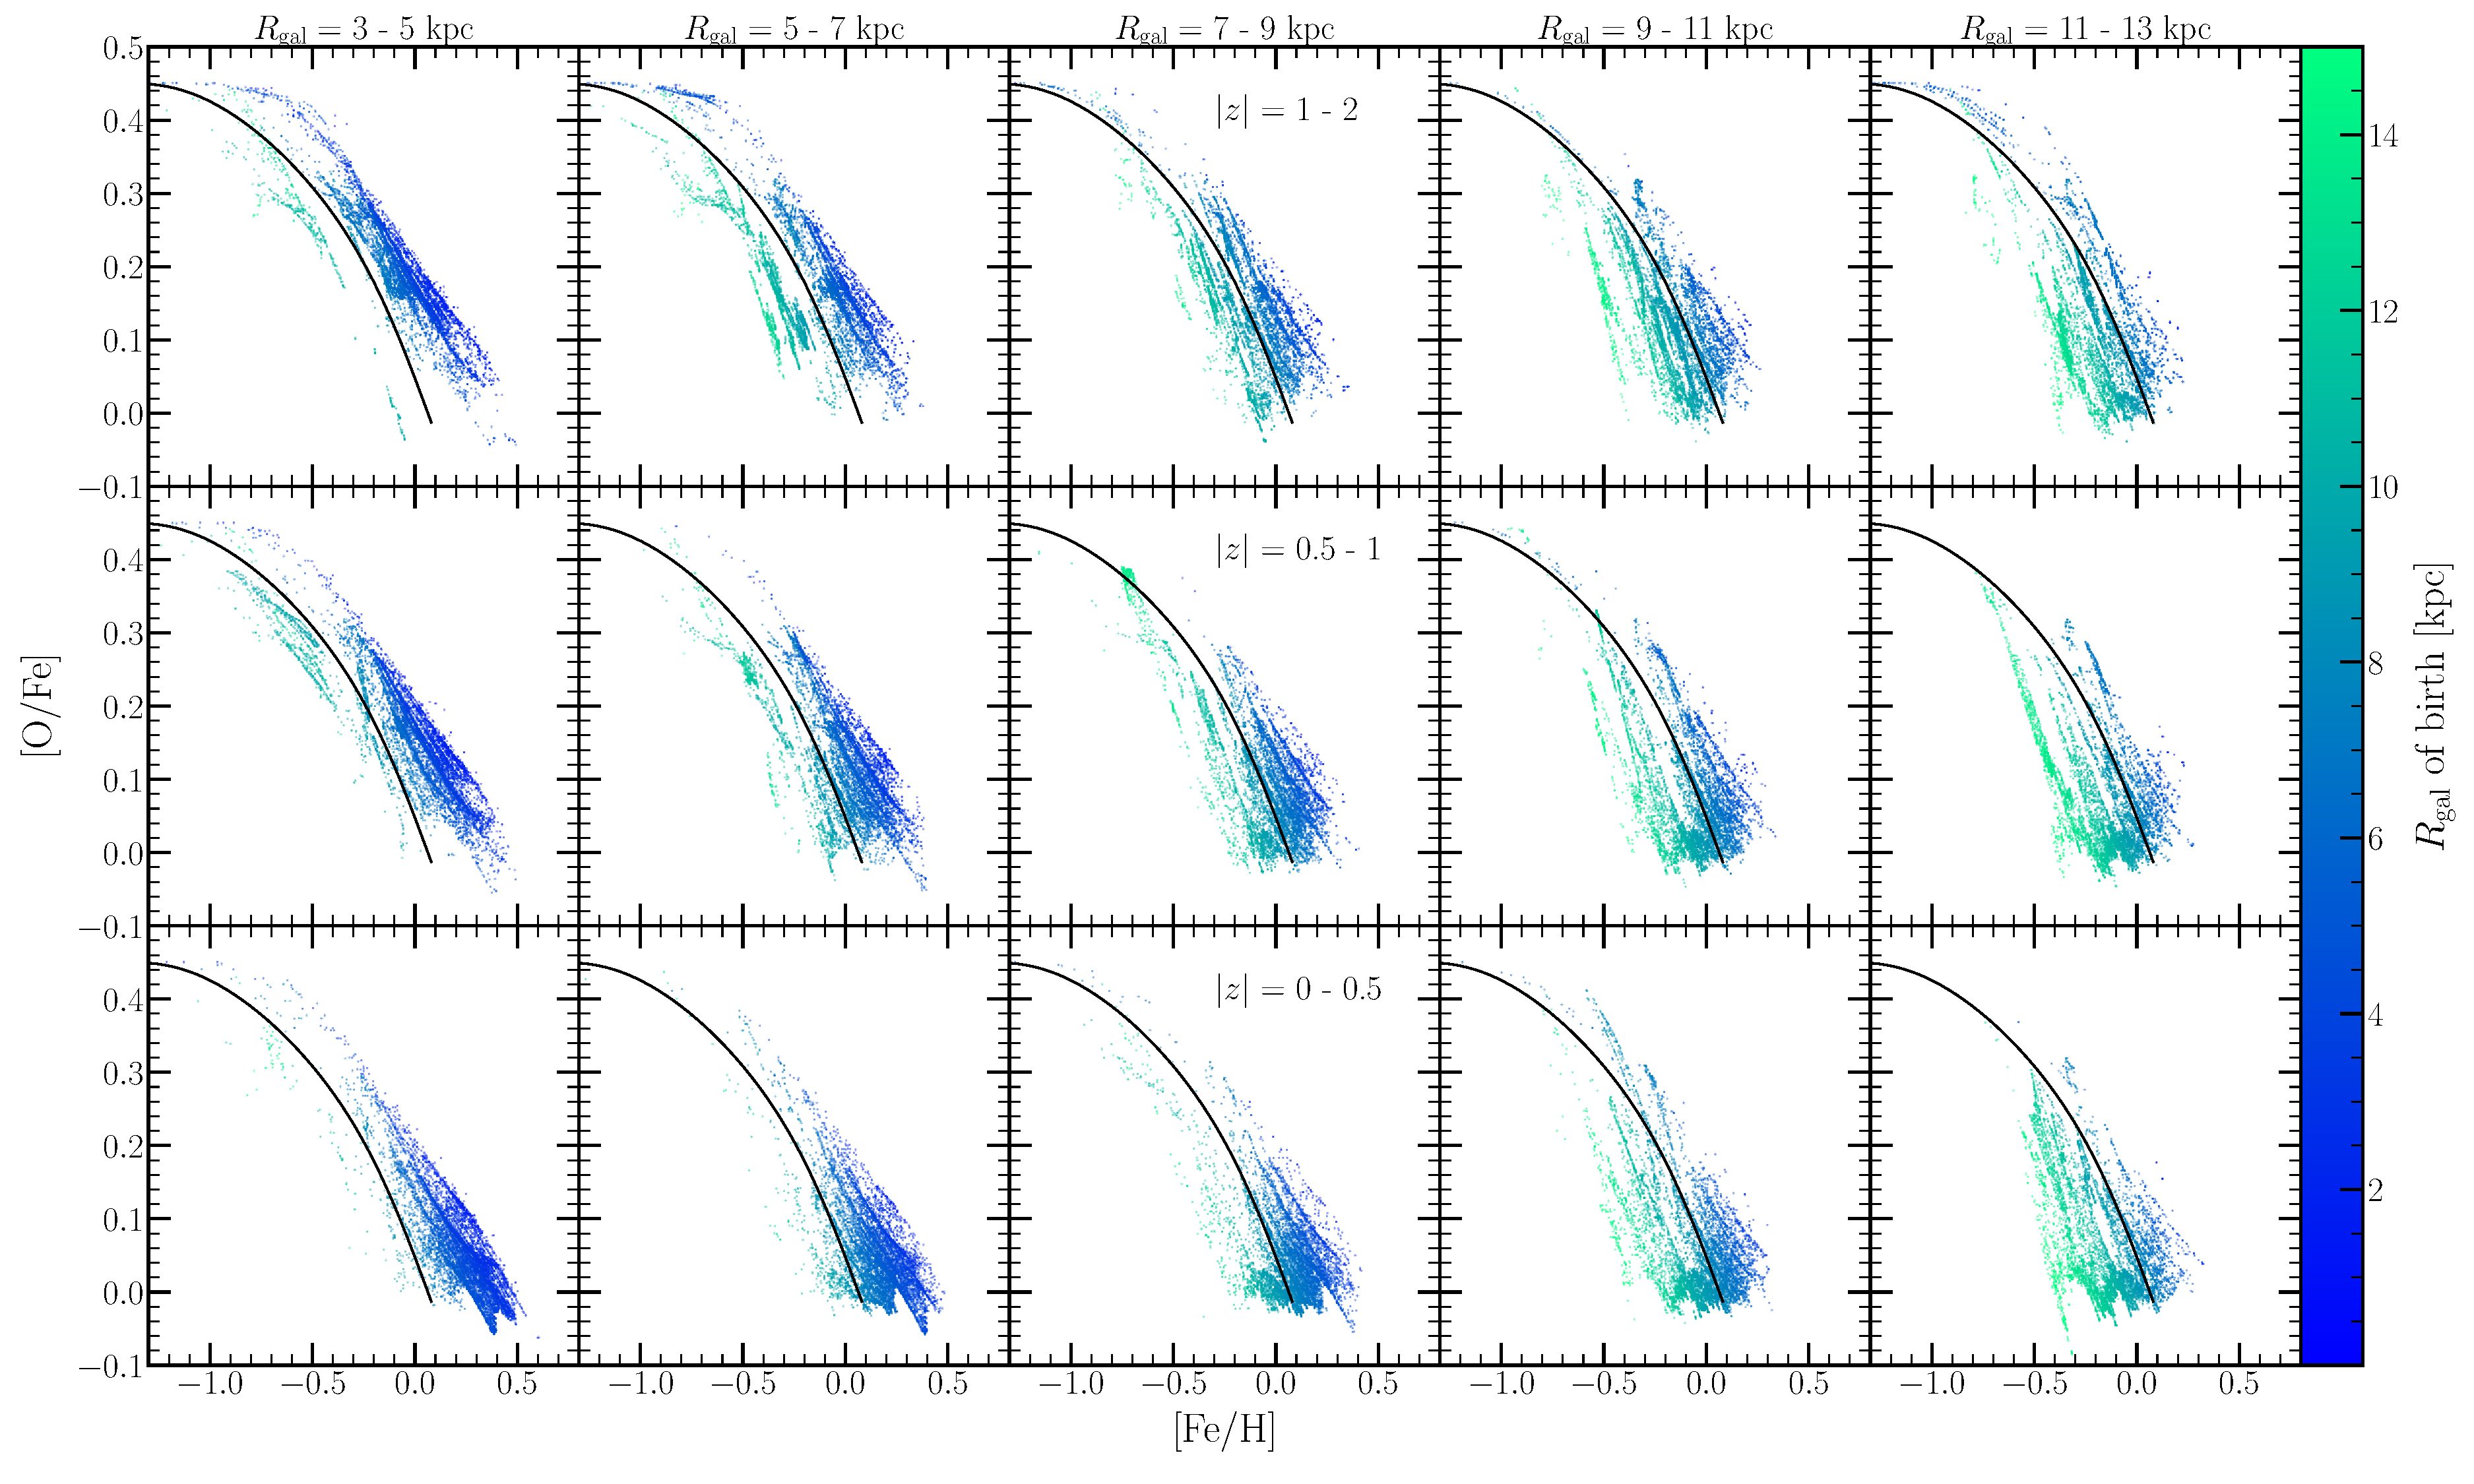
\includegraphics[scale = 0.28]{ofe_feh_scatterplot_insideout.pdf} 
\caption{[O/Fe]-[Fe/H] diagrams for 15 galactic regions spanning five bins in 
$R_\text{gal}$ and~$\left|z\right|$. Each region has its own panel, with radial 
bins shown in columns denoted at the top of the figure, and with 
$\left|z\right|$ bins shown in rows denoted in text in the middle column 
panels. In each panel, we plot $N$ = 10,000 points sampled from our simulated 
stellar populations in each region predicted by our inside-out SFH, where the 
probability of sampling is proportional to the present-day mass of each stellar 
population. In all panels points are color-coded according to the 
Galactocentric radius of birth of the stellar population. For reference, we 
plot in a solid black line in all panels the gas-phase [O/Fe]-[Fe/H] track 
predicted by the same SFH in the $R_\text{gal}$ = 8 kpc annulus, but with the 
post-processing migration model; this curve is the same in all panels. }
\label{fig:ofe_feh_diagram} 
\end{figure*} 

\begin{itemize} 
	\item Predicted [O/Fe]-[Fe/H] tracks for the diffusion model show 
	significant deviations from the post-processing model, and these 
	variations are due to the SN Ia rate varying in response to radial 
	migration. This challenges the assumption that stars don't contribute to 
	nucleosynthetic yields beyond their birth radius; that is, if a 
	statistically significant fraction of stars are expected to migrate 
	significantly from their birth radius when they're young ($\lesssim$ 2 
	Gyr), this approximation is invalid. This is proof of concept that the 
	radial migration of yields can occur as a consequence of the radial 
	migration of stars. 

	\item For each zone,~\texttt{VICE} provies in its outputs the rates of 
	infall and star formation, the mass of the ISM, and the relevant 
	abundance information for each element along with the associated 
	MDFs at the final timestep. To determine the SN Ia rates, we therefore 
	have to approximate from the output. 
	\begin{itemize} 
		\item The time-derivative of the mass of Fe in a given annulus is 
		given by: 
		\begin{equation}
		\dot{M}_\text{Fe} \approx y_\text{Fe}^\text{CC}\dot{M}_\star + 
		y_\text{Fe}^\text{Ia}\langle\dot{M}_\star\rangle_\text{Ia} - 
		\frac{M_\text{Fe}}{M_g}\dot{M}_\star(1 + \eta(R_\text{gal}) - r) 
		\end{equation} 
		where this is an approximation because in detail, there is a small 
		contribution from AGB stars, and the recycling in the simulation is 
		done continuously, whereas here we simply take $r \approx$ 0.4 
		(appropriate for a~\citetalias{Kroupa2001} IMF;~\citealp{Weinberg2017}). 
		This equation can be derived from the~\citet{Weinberg2017} analytic 
		models assuming CCSN and SN Ia enrichment for Fe with instantaneous 
		recycling of previously produced Fe.~\texttt{VICE}'s science 
		documentation could also be referenced here; it has a nice detailed 
		section on its treatment of each term in handling enrichment rates 
		\footnote{
			\url{https://vice-astro.readthedocs.io/en/latest/science_documentation/enrichment/index.html}
		}. 
		Rearranging this for the term describing the rate of injection due to 
		SNe Ia events, and normalizing by $M_\text{Fe}$ yields the following 
		proxy with units of frequency: 
		\begin{equation} 
		\frac{
			y_\text{Fe}^\text{Ia}\langle\dot{M}_\star\rangle_\text{Ia}
		}{
			M_\text{Fe} 
		} \approx 
		\frac{\dot{M}_\text{Fe}}{M_\text{Fe}} - y_\text{Fe}^\text{CC}\frac{
			\dot{M}_\star 
		}{
			M_\text{Fe} 
		} + \frac{\dot{M}_\star}{M_g}(1 + \eta(R_\text{gal}) - r) 
		\label{eq:ia_rate_proxy} 
		\end{equation} 
		This term on the left-hand side can be substituted with 
		$m_\text{Fe}^\text{Ia}\dot{N}_\text{Ia}/M_\text{Fe}$, where 
		$m_\text{Fe}^\text{Ia}$ is the average mass of Fe produced by a single 
		SN Ia event, and $\dot{N}_\text{Ia}$ is the SN Ia rate itself. For 
		this reason, this equation constitutes a straight-forward proxy for 
		the SN Ia rate at any given time. This is the proxy that's plotted in 
		the right-hand panel of~Fig.~\ref{fig:tracks}, with multilicative 
		factors added for visual clarity. 
	\end{itemize} 

	\item Some folks have assumed tracks in the [O/Fe]-[Fe/H] plane to infer 
	birth radii for observed stars. We caution against inferring birth radii 
	in this way for high-$\alpha$ stars, because there radial migration may 
	cause one to infer a considerably wrong birth radius, provided they're 
	assuming a post-processing migration model. This however doesn't seem to 
	affect the low-$\alpha$ sequence. It's possible that an additional 
	dimension such as age could mitigate these issues. 

	\item Variability in the SN Ia rate shows high-amplitude on Gyr timescale, 
	low-amplitude white-noise on shorter timescales. In general the 
	time-averaged rates follow the expectation from the post-processing model. 
	Fractional amplitude of variability increases with Galactocentric radius. 

	\item Demonstrate in the next section that this is a means with which to 
	form $\alpha$-rich and $\alpha$-poor stars - or rather Fe-poor and 
	Fe-rich, respectively. 

	\item Fig.~\ref{fig:ofe_feh_diagram} shows a scatter plot of 10,000 
	randomly sample stellar populations in five bins of $R_\text{gal}$ and 
	three bins of $\left|z\right|$ ($R_\text{gal}$ = 3 - 5 kpc, 5 - 7 kpc, 
	7 - 9 kpc, 9 - 11 kpc, and 11 - 13 kpc; $\left|z\right|$ = 0 - 0.5 kpc, 
	0.5 - 1 kpc, and 1 - 2 kpc). These are the same bins and same scheme for 
	organizing the panels as in Fig. 4 of~\citet{Hayden2015}. 

	\item The width of the low-$\alpha$ sequence predicted by the model comes 
	from radial migration, in agreement with the prediction 
	of~\citet{Schoenrich2009}. 

	\item The low-$\alpha$ sequence shifts from a high [Fe/H] locus at small 
	$R_\text{gal}$ to low [Fe/H] at high~$R_\text{gal}$, in agreement with the 
	observed distributions in APOGEE presented in~\citet{Hayden2015}. 

	\item High-$\alpha$ stars are most prevalent at low~$R_\text{gal}$ and 
	high~$\left|z\right|$, and conversely for the low-$\alpha$ stars, also 
	in agreement with~\citet{Hayden2015}. 
	\begin{itemize} 
		\item Similar results are found for different SFHs. This suggests that 
		this observed result is a natural consequence of stellar migration. 

		\item Only minor difference worth noting is that the starburst models 
		predict a slightly higher characteristic [O/Fe] ($\sim$+0.1) for the 
		low-$\alpha$ sequence. This is a natural consequence of the starburst. 
	\end{itemize} 
\end{itemize} 

\section{The Age-[$\alpha$/Fe] Relation} 
\label{sec:age_alpha} 

\begin{figure*} 
\centering 
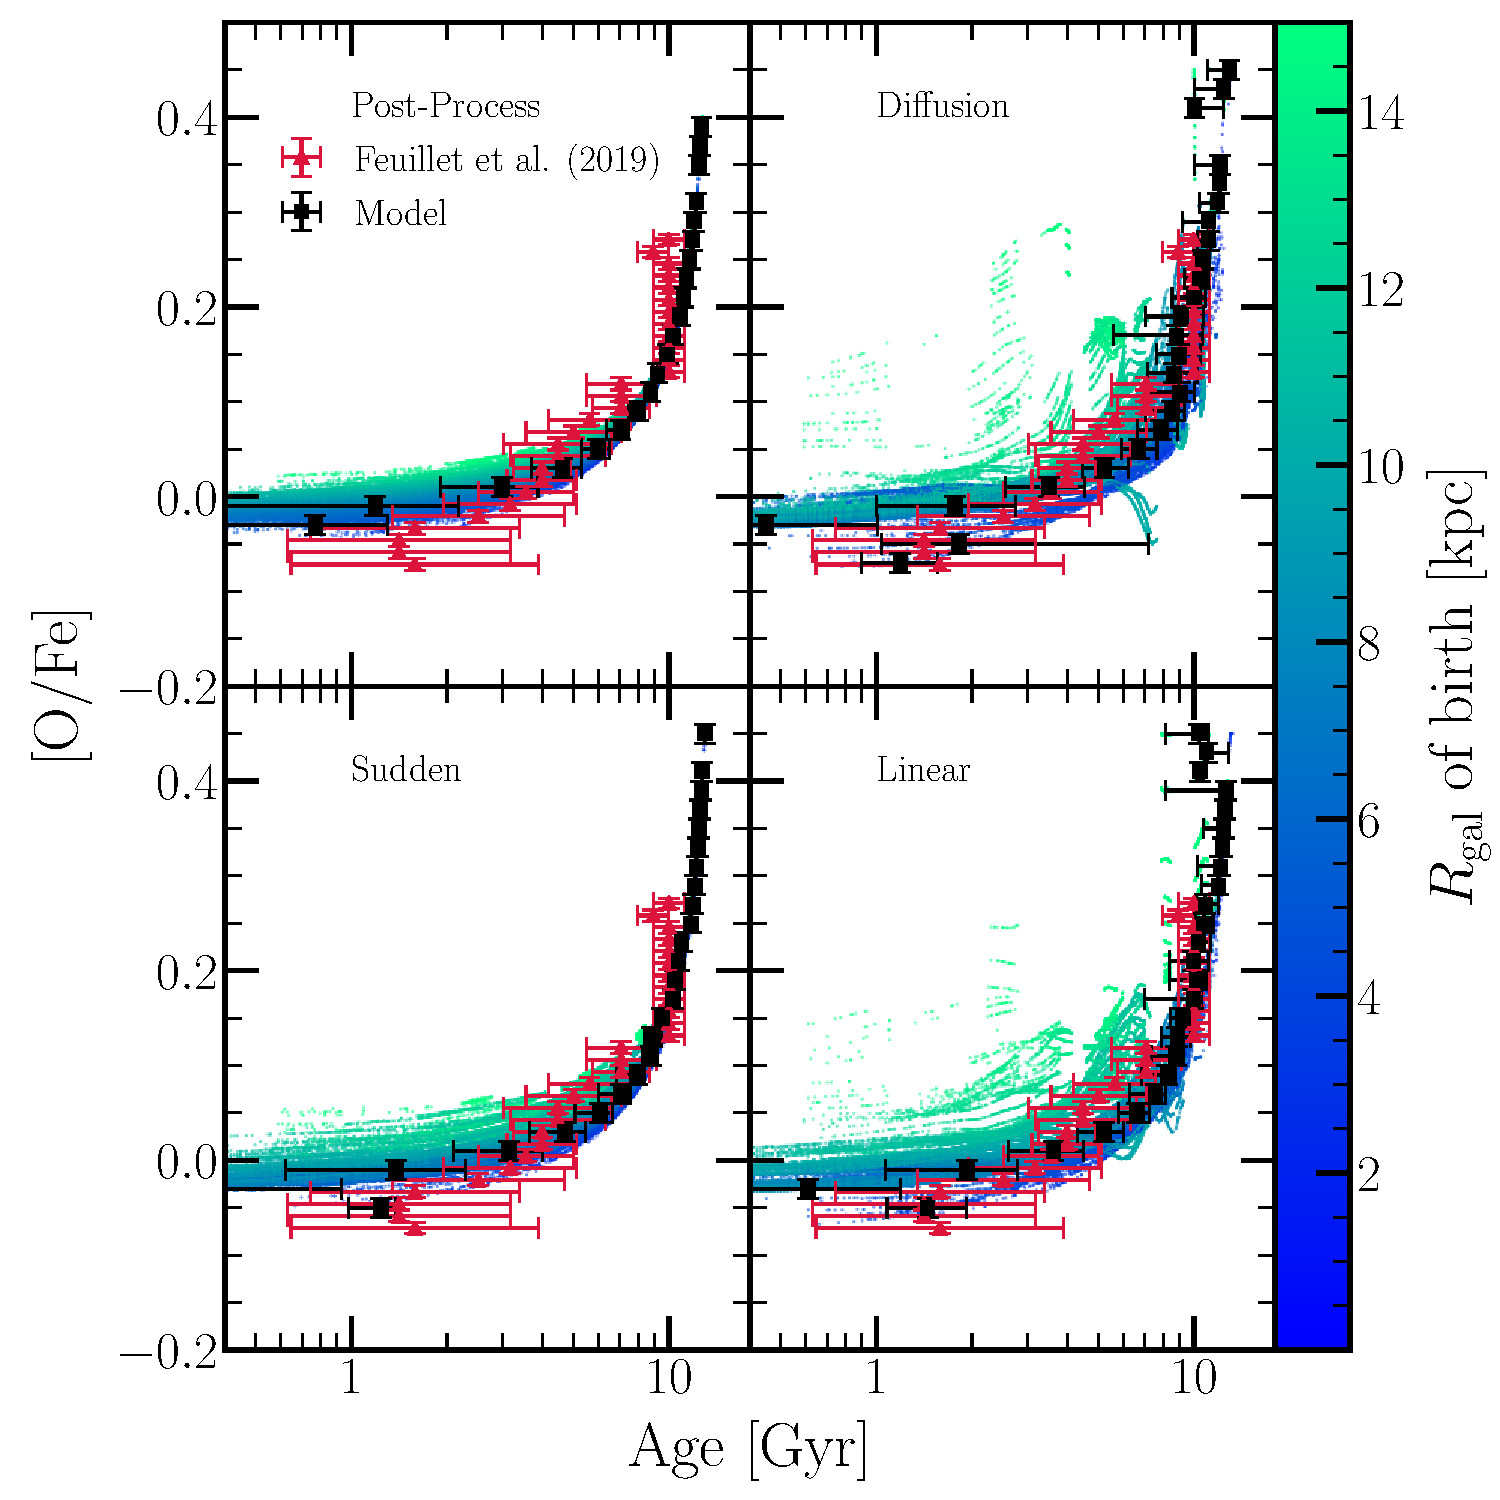
\includegraphics[scale = 0.5]{age_ofe_migration_comparison.pdf} 
\caption{A comparison of the predicted age-[O/Fe] relation for the solar 
annulus ($R_\text{gal}$ = 7 - 9 kpc and $\left|z\right|\leq$ 0.5 kpc) 
between the post-processing (upper left), diffusion (upper right), sudden 
(lower left), and linear (lower right) migration models, assuming our 
inside-out SFH and $\tau_\star^\text{mol} = (\text{2 Gyr})(t/t_0)^{1/2}$. 
Red triangles and error bars denote the observed mean age and dispersion 
thereof in bins of [O/Fe] as reported by~\citet{Feuillet2019}; here we include 
only the bins containing at least 15 stars. Black squares denote the 
mass-weighted median age in 0.02-dex bins in [O/Fe], with error bars denoting 
the 16th and 84th percentiles of the mass-weighted age distribution in 
those bins. Points in the background denote each individual stellar population 
from the simulation with a final position in the solar annulus, color-coded 
according to their Galactocentric radius of birth. } 
\label{fig:age_alpha_migration_comparison} 
\end{figure*} 

\begin{figure*} 
\centering 
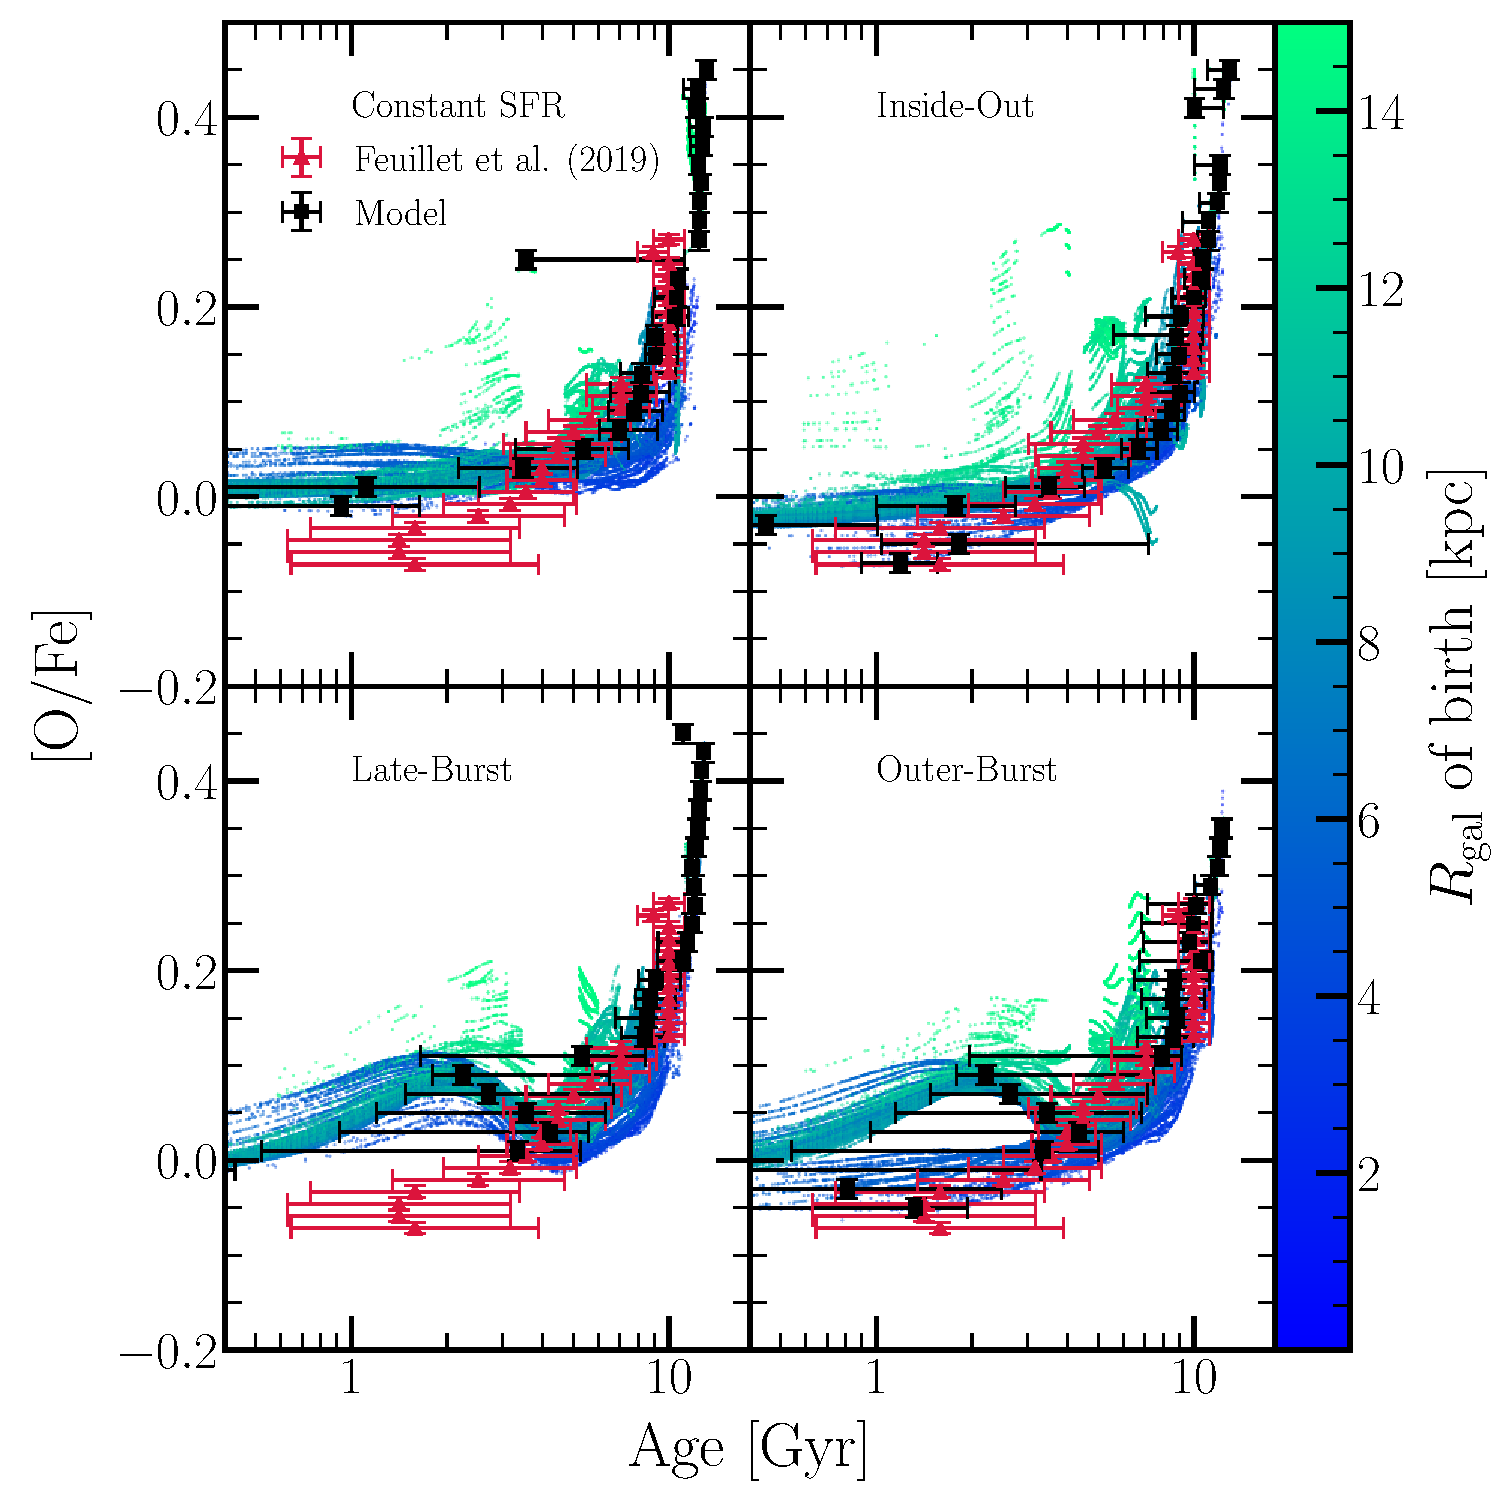
\includegraphics[scale = 0.5]{age_ofe_sfh_comparison.pdf} 
\caption{The same as Fig.~\ref{fig:age_alpha_migration_comparison}, instead 
comparing the impact of our constant (upper left), inside-out (upper right), 
late-burst (lower left), and outer-burst (lower right) SFHs, assuming diffusion 
migration and $\tau_\star^\text{mol} = (\text{2 Gyr})(t/t_0)^{1/2}$. }
\label{fig:age_alpha_sfh_comparison} 
\end{figure*} 

\begin{figure*} 
\centering 
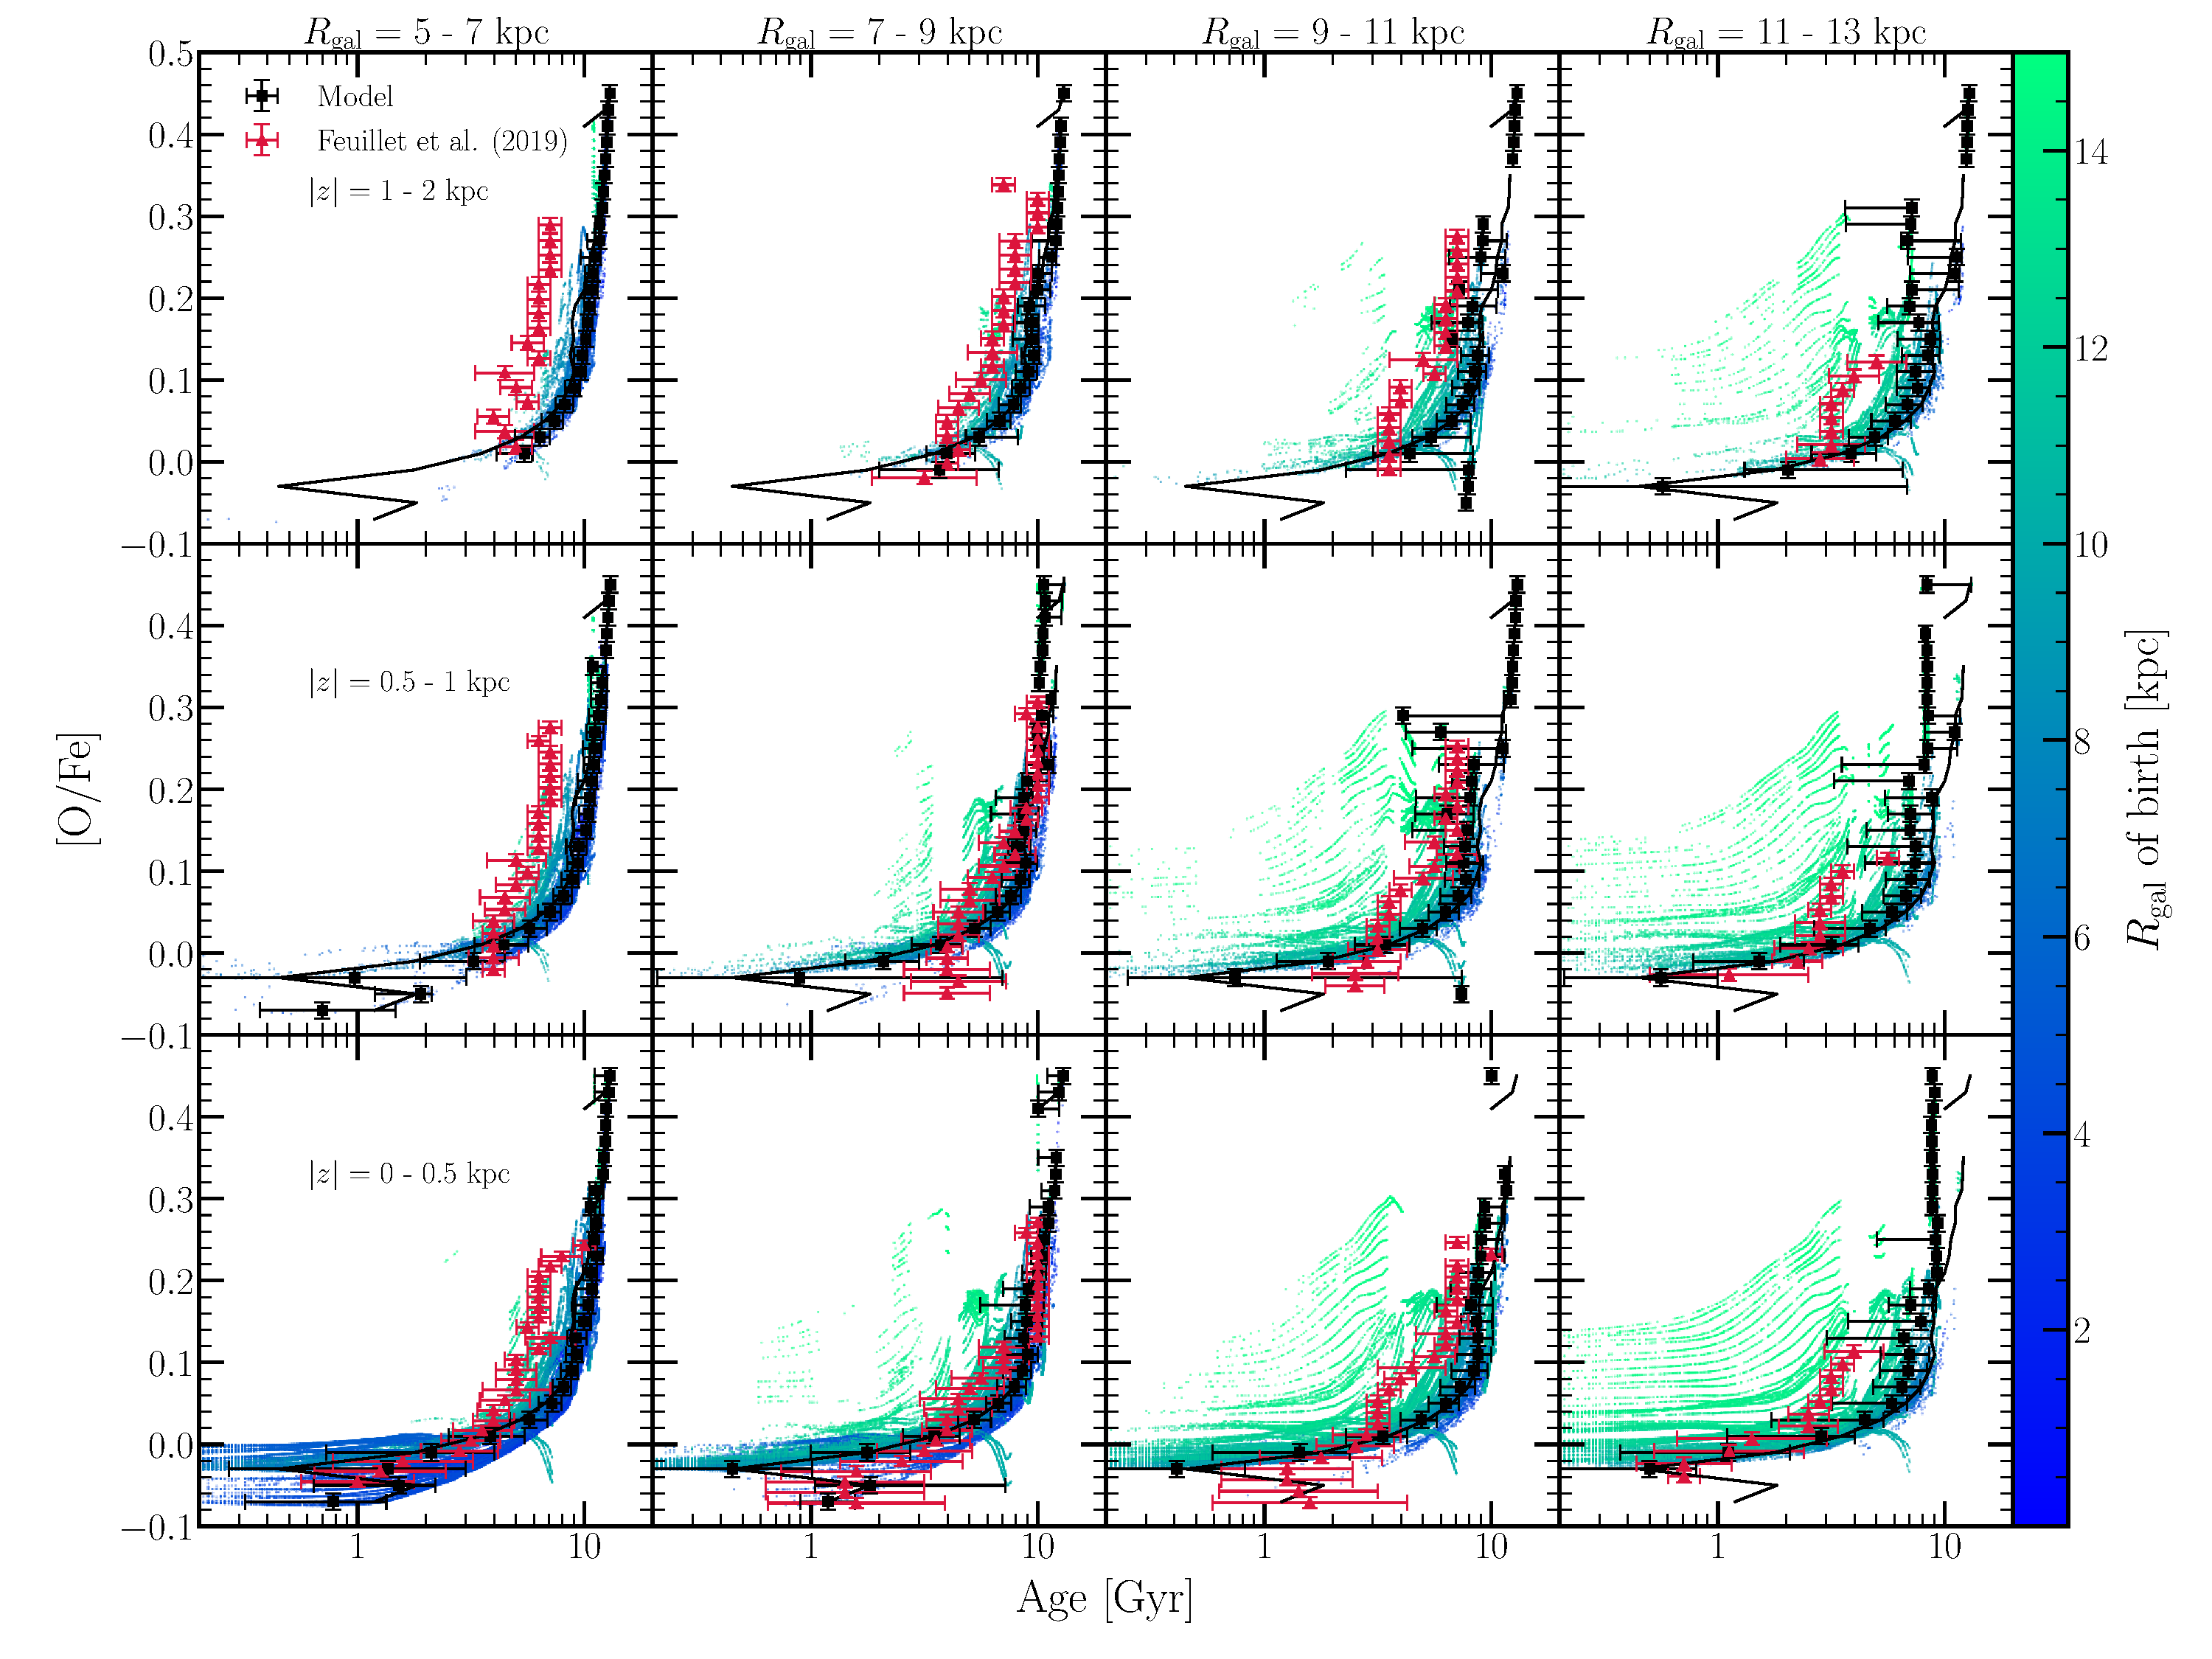
\includegraphics[scale = 0.32]{age_alpha_regions.pdf} 
\caption{The age-[O/Fe] relation in difference galactic regions predicted by 
our inside-out SFH with $\tau_\star^\text{mol} = (\text{2 Gyr})(t/t_0)^{1/2}$ 
and diffusion migration. Bins in Galactocentric radius are shown in columns, 
and labeled at the top. Bins in the height $\left|z\right|$ above/below the 
disk midplane are shown in rows, noted in the left-hand column. Red triangles 
and error bars denote the observed mean age and dispersion thereof in bins of 
[O/Fe] as reported by~\citet{Feuillet2019}; here we include only the mass bins 
containing at least 15 stars. Black squares denote the mass-weighted median 
age in 0.02-dex bins in [O/Fe], with error bars denoting the 16th and 84th 
percentiles of the mass-weighted age distribution in those bins. Points in the 
background denote each individual stellar population from the simulation with 
a final position in that Galactic region, color-coded according to their 
Galactocentric radius of birth. } 
\label{fig:age_alpha_regions} 
\end{figure*} 

\begin{itemize} 
	\item \citet{Feuillet2019} make use of APOGEE DR14 stars where there are 
	Gaia parallax measurements available~\citep{GaiaDR2}. With their spatial 
	cuts, the final sample consisted of 77,562 stars. In bins of [O/Fe], they 
	assume a gaussian age distribution, and fit the mean and standard deviation 
	to the observed sample. Because they assume a gaussian, they would report 
	an equal mean and median. 

	\item The stellar populations from our simulations have different masses, 
	so the age-distributions must be weighted by mass, since that scales with 
	the number of stars that each stellar population represents. 

	\item Our age distributions in the vast majority of [O/Fe] bins are 
	highly non-gaussian, so we compare to~\citet{Feuillet2019} based on the 
	predicted mass-weighted median age in [O/Fe] bins (i.e. the age which 50\% 
	of the stellar mass in a given bin is younger than). For these reasons the 
	comparison between our simulations and~\citet{Feuillet2019} isn't exactly 
	one-to-one. 
\end{itemize}

\subsection{The Impact of Radial Migration} 
\label{sec:age_alpha:migration} 
\begin{itemize} 
	\item Fig.~\ref{fig:age_alpha_migration_comparison} shows a comparison 
	between the predicted age-[$\alpha$/Fe] relations in the solar annulus for 
	our four migration models assuming our inside-out SFH. 

	\item All models show reasonable agreement with the~\citet{Feuillet2019} 
	data; the population-averaged trend appears insensitive to the assumed 
	migration model. 

	\item Diffusion predicts the most intrinsic scatter, followed by linear, 
	then sudden, then post-processing. Further demonstration that under 
	certain migration models, the radial migration of nucleosynthetic yields 
	is statistically significant. 

	\item This mechanism can produce populations of Fe-poor or Fe-rich stars, 
	which can be misinterpreted as $\alpha$-rich or $\alpha$-poor stars. Due 
	to young stars migrating into or out of a given annulus, the SN Ia rate 
	may be higher or lower than the expectation from a post-processing 
	migration model. If this difference in the SN Ia rate is sustained for of 
	order one depletion time, the ISM will be either Fe-poor or Fe-rich, and 
	the stars that form there will inherit that composition.\footnote{
		{\color{red} Potentially note the~\citet{Weinberg2017} definition: 
		$\tau_\text{dep} \equiv \tau_\star/(1 + \eta - r)$. Even with 
		$\tau_\star$ as high as~$\sim$5 Gyr at large Galactocentric radii, 
		depletion times are still short due to the high values of $\eta$ 
		there.}
	} The stars that form out of that patch of ISM can then migrate to the 
	solar annulus. This effect is most significant at large Galactocentric 
	radii where the fractional amplitude of the variability in the SN Ia rate 
	is largest, and for that reason the young Fe-poor population predicted by 
	our diffusion model originates at large radii ($\gtrsim$ 12 kpc). 

	\item \citet{SilvaAguirre2018} demonstrated that the observed young 
	$\alpha$-rich stars in the solar annulus have kinematics similar to the 
	rest of the high-$\alpha$ population, and suggested that this may be the 
	result of stellar mergers or mass transfer events, producing a population 
	of truly old stars masquerading as young stars. This would imply that the 
	observed young $\alpha$-rich population is actually just older, 
	high-$\alpha$ stars that have gone through some special class of stellar 
	evolution. Our model predicts intrinsically young, Fe-poor stars to 
	explain the observations, but these interpretations are not mutually 
	exclusive. Ascertaining the origins of this population therefore has 
	implications for which of the migration models investigated here is the 
	most realistic. 
\end{itemize} 

\subsection{The Impact of the Star Formation SFH} 
\label{sec:age_alpha:sfh} 
\begin{itemize} 
	\item Fig.~\ref{fig:age_alpha_sfh_comparison} shows a comparison between 
	the predicted age-[$\alpha$/Fe] relations in the solar annulus for our 
	four SFHs assuming diffusion migration. 

	\item Constant and inside-out SFHs describe the observed data the best. 
	Both late starburst models show a population-averaged increase in 
	[$\alpha$/Fe] at young ages which is not observed in the data. This 
	challenges the results of~\citet{Isern2019} and~\citet{Mor2019}, 
	suggesting that these results on the Milky Way recent SFH are not 
	consistent with chemical evolution models. 

	\item Below [O/Fe]~$\approx$ +0.1, the~\citet{Feuillet2019} data seem to 
	follow a slightly steeper age-[$\alpha$/Fe] than our inside-out model 
	predicts. This likely points to inaccuracies in the detailed form of the 
	SFH or the SN Ia DTD, both of which are within the uncertainties of these 
	models. 
\end{itemize} 

\subsection{Beyond the Solar Annulus} 
\label{sec:age_alpha:beyond_solar_annulus} 
\begin{itemize} 
	\item Fig.~\ref{fig:age_alpha_regions} presents a comparison of our 
	simulation data to the~\citet{Feuillet2019} observational data in 12 
	Galactic regions assuming the inside-out SFH. 

	\item In the disk, the inside-out SFH is a reasonable description of the 
	data for ages~$\lesssim$ 5 Gyr, above which the median ages are 
	overpredicted relative to~\citet{Feuillet2019}. Far from the midplane, our 
	model overpredicts the ages at nearly all abundances 
	where~\citet{Feuillet2019} have data, with the exception of the 
	$R_\text{gal}$ = 7 - 9 kpc and $\left|z\right|$ = 0.5 - 1 kpc region. 

	\item Differences in ages are interesting though - nearly everywhere we 
	overpredict ages relative to~\citet{Feuillet2019}, their data are 
	reasonably described by the stellar populations from our simulations that 
	we would classify as Fe-poor. Especially noticeable in the $R_\text{gal}$ 
	= 5 - 7 kpc, $\left|z\right|\leq$ 0.5 regions (i.e. lower-left panel), 
	where the observed data also show an abrupt increase in age near the 
	maximum [O/Fe] ratio of one particular Fe-poor population, with one data 
	point that agrees with the population-averaged trend from the simulation. 
	\begin{itemize}
		\item Taking the~\citet{Feuillet2019} data at face value, this would 
		suggest that our simulation is overpredicting the rate of Fe injection 
		from SN Ia, implying a SN Ia DTD whose characteristic timescales are 
		longer than we employ here, thus slowing the decrease of [$\alpha$/Fe] 
		with time. 

		\item \citet{Feuillet2019} made use of APOGEE DR14 data for which 
		Gaia parallax measurements are available. With their quality cuts the 
		final sample consisted of 77,562 stars. Taking the simulation results 
		at face value, this would suggest that APOGEE+Gaia target selection 
		favors the stars we would classify as Fe-poor. 
	\end{itemize} 
\end{itemize} 

\section{The Age-Metallicity Relation} 
\label{sec:amr} 

\begin{figure*} 
\centering 
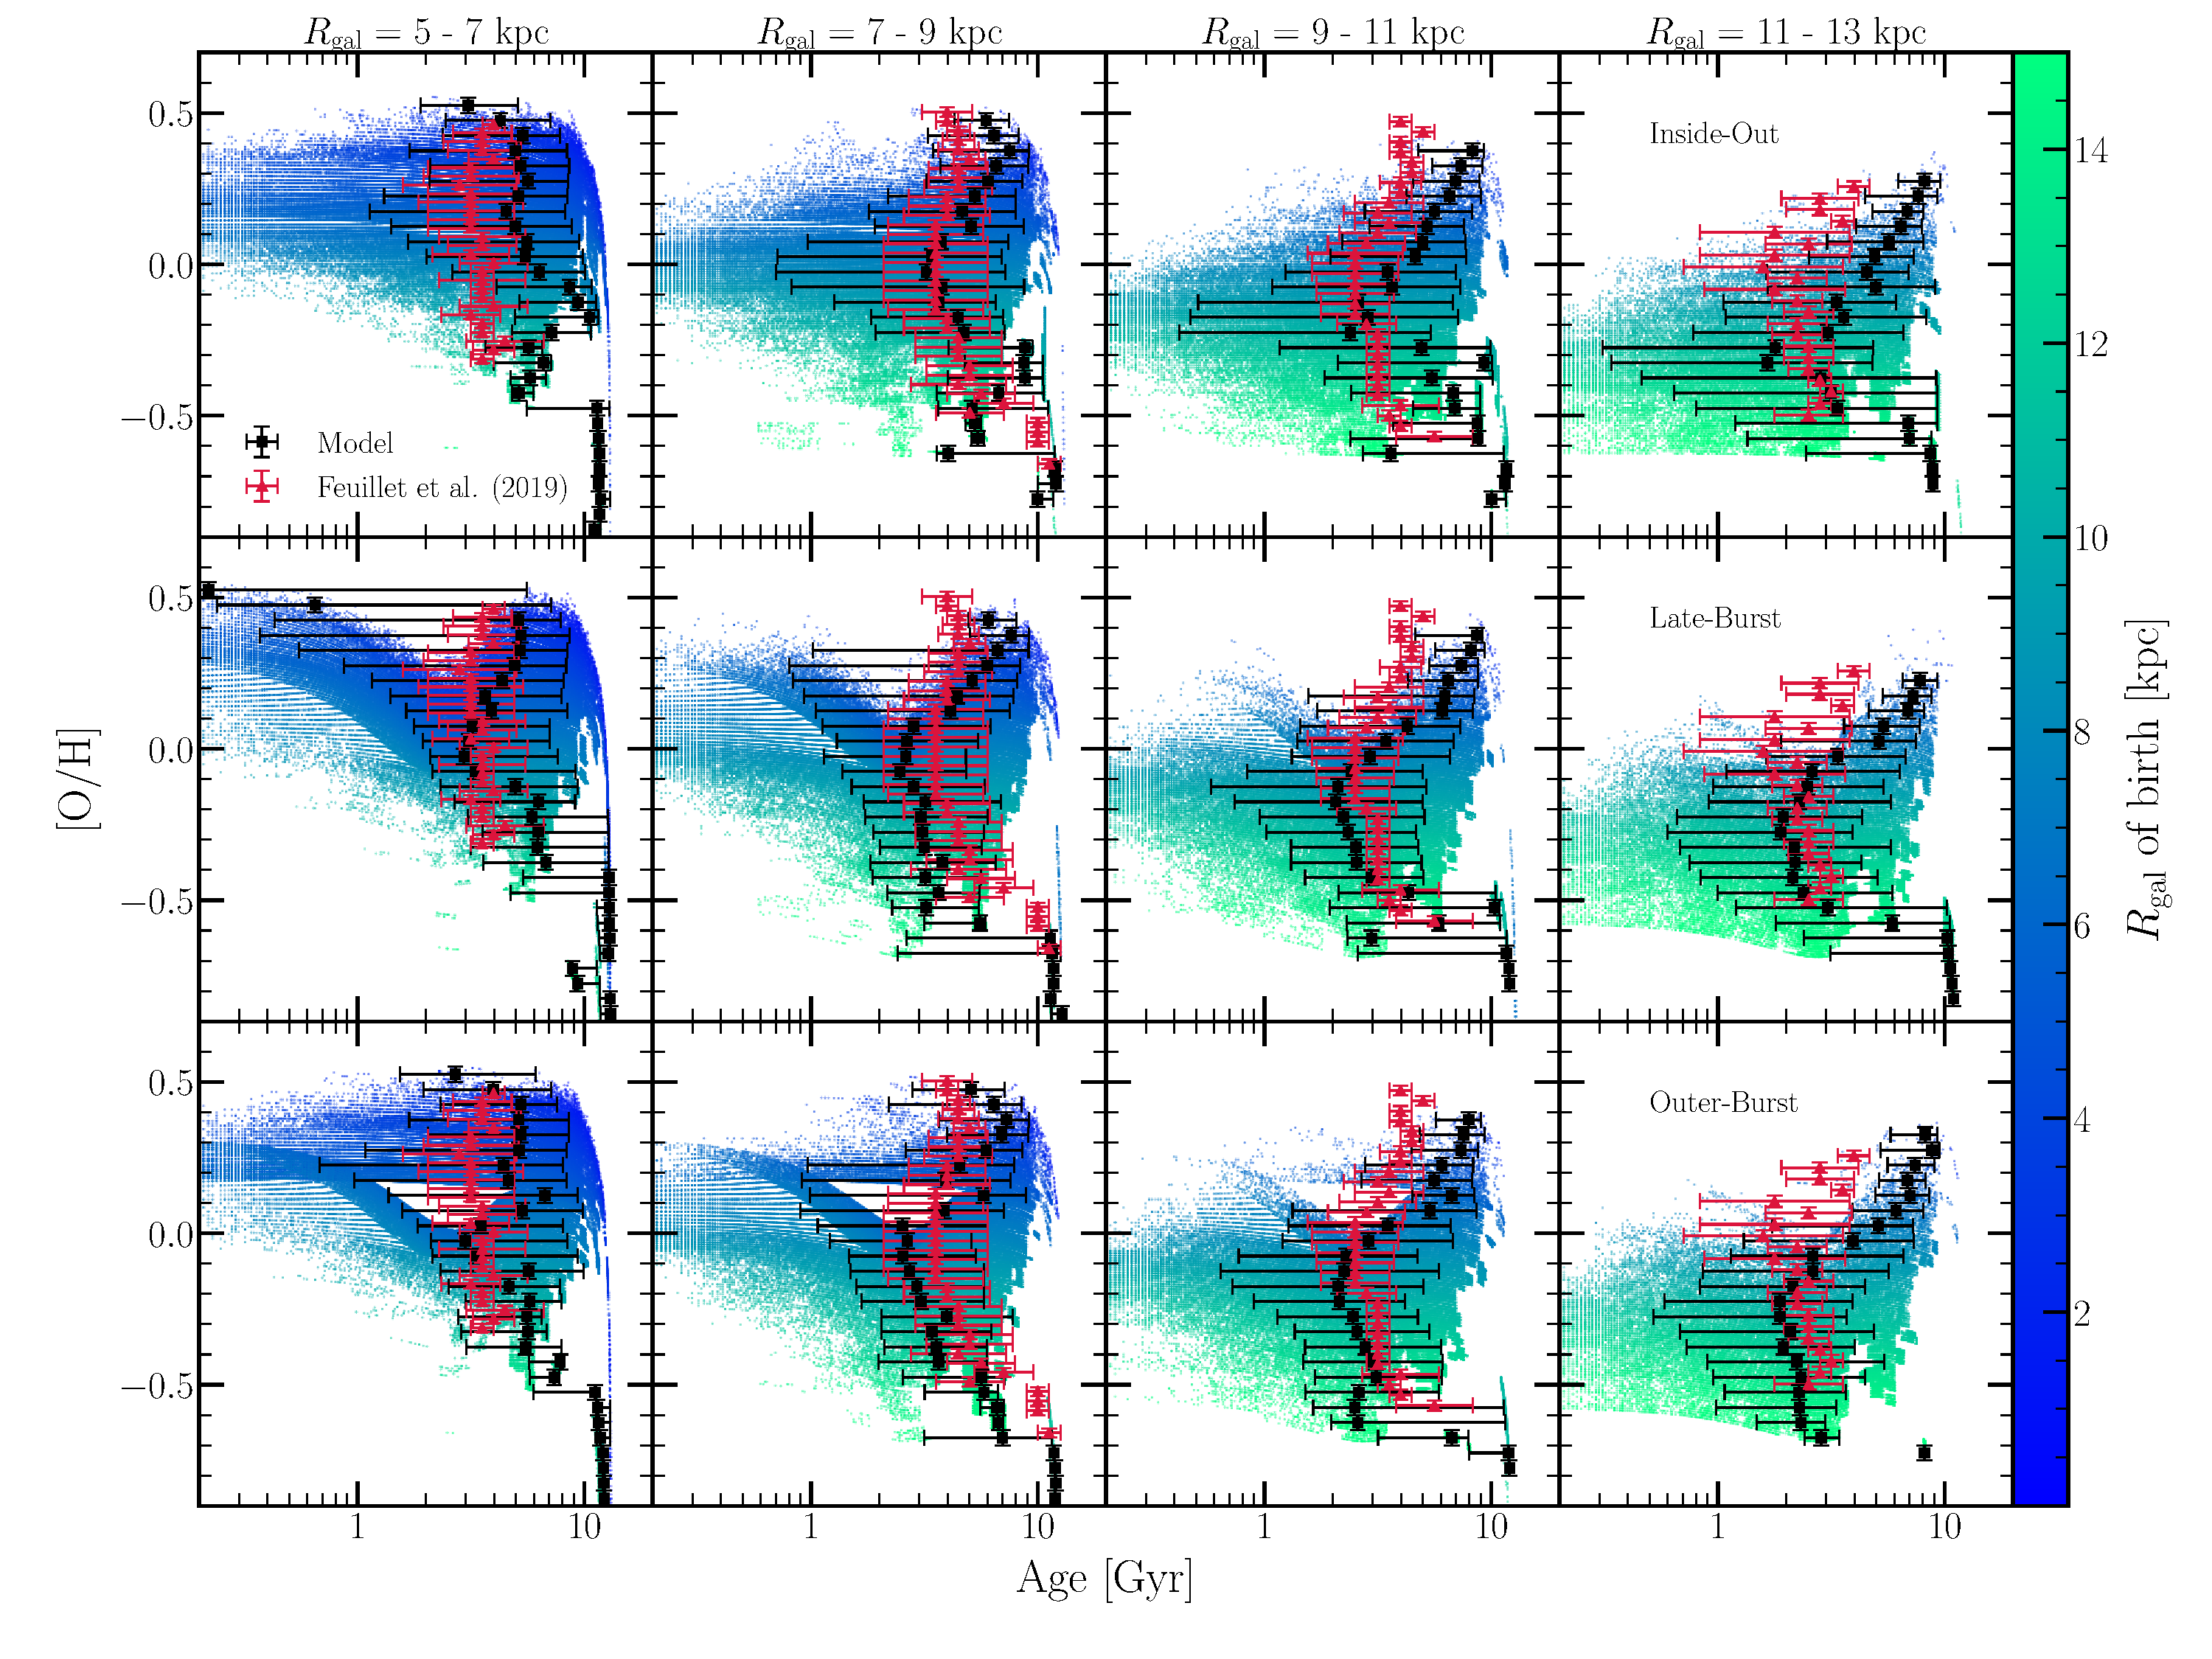
\includegraphics[scale = 0.32]{age_oh_comparison.pdf} 
\caption{The age-[$\alpha$/H] relation predicted by our constant (top), 
inside-out (top middle), late-burst (bottom middle), and outer-burst (bottom) 
SFHs for $R_\text{gal}$ = 5 - 7 kpc (left), 7 - 9 kpc (left middle), 9 - 11 
kpc (right middle), and 11 - 13 kpc (right). Each panel plots only the 
$\left|z\right|\leq$ 0.5 kpc population. Background points, red triangles with 
error bars, and black squares with error bars are as in 
Fig.~\ref{fig:age_alpha_regions}, but with our binned, simulation quantified 
in 0.05-dex bins in [O/H]. } 
\label{fig:age_oh_comparison}
\end{figure*} 

\begin{figure*} 
\centering 
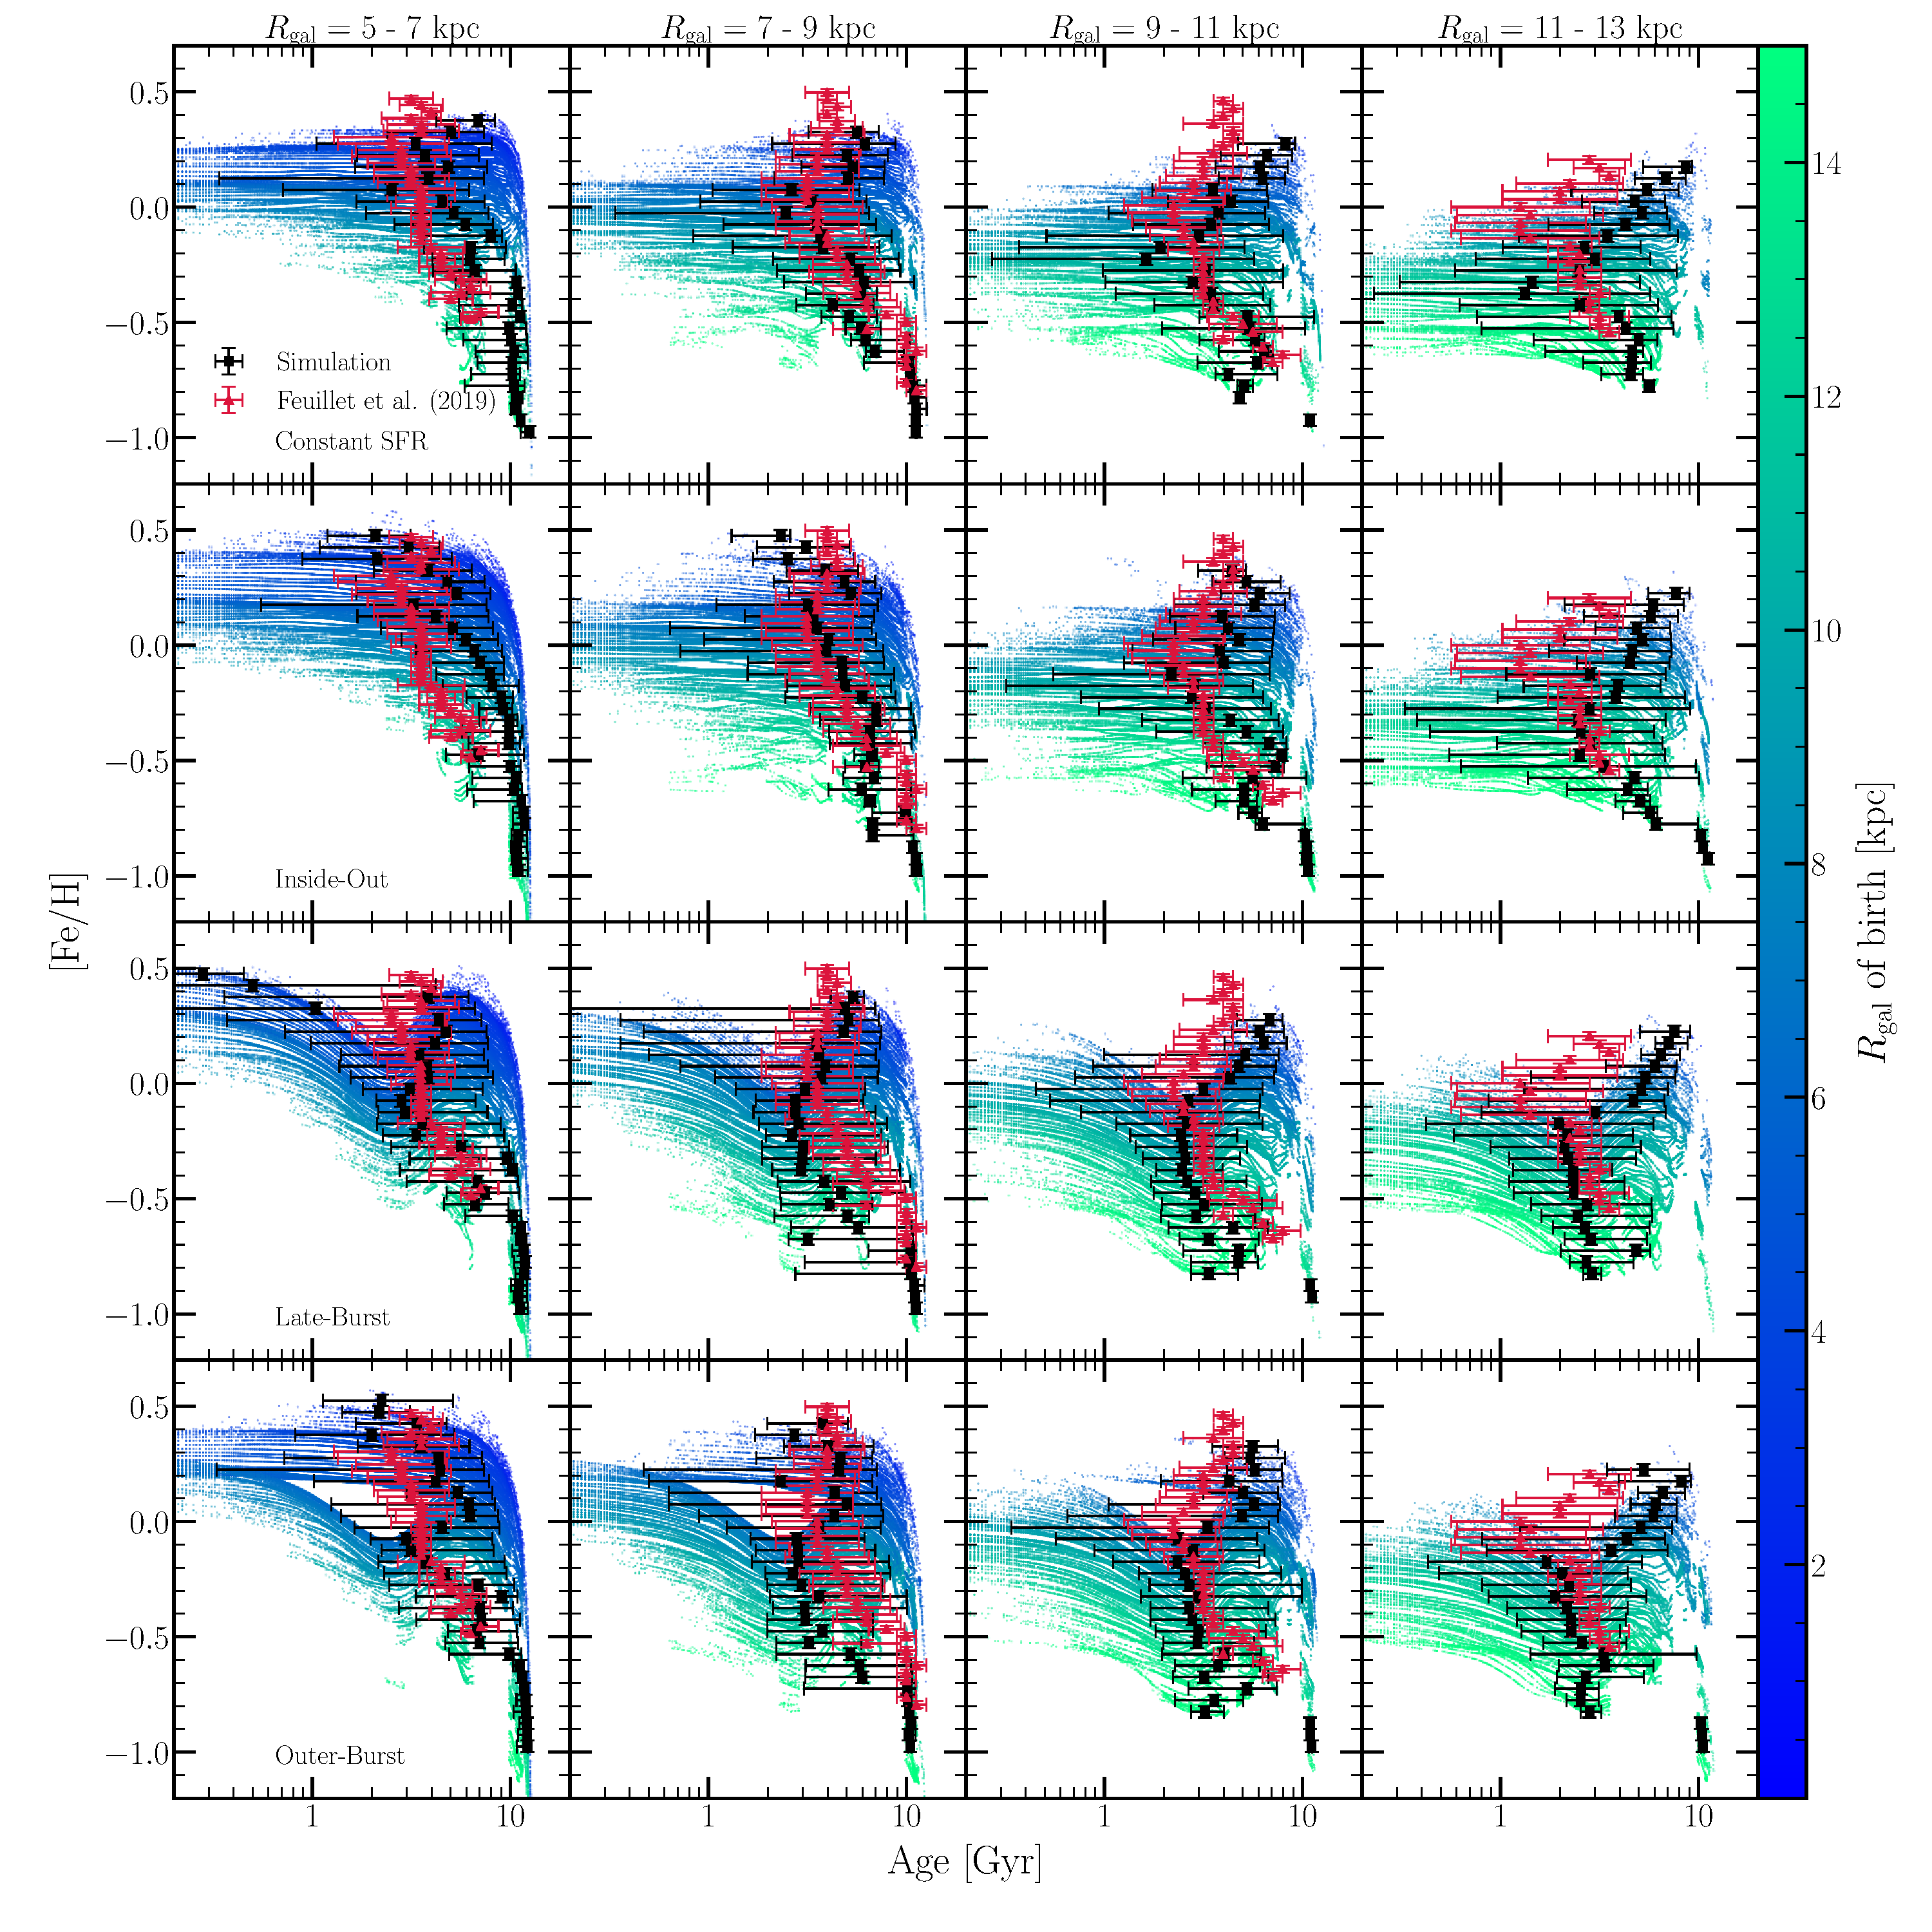
\includegraphics[scale = 0.32]{age_feh_comparison.pdf} 
\caption{The same as Fig.~\ref{fig:age_oh_comparison}, but for the age-[Fe/H] 
relation. } 
\label{fig:age_feh_comparison} 
\end{figure*} 

\begin{itemize} 
	\item Fig.~\ref{fig:age_oh_comparison} shows a comparison of the 
	predicted age-[O/H] for $\left|z\right|\leq$ 0.5 stars in four bins in 
	Galactocentric radius between our four fiducial SFHs and 
	the~\citet{Feuillet2019} data. Fig.~\ref{fig:age_feh_comparison} shows 
	the same comparison but for the age-[Fe/H] relation. 

	\item For a constant SFR, our model predicts a non-monotonic AMR at all 
	radii for both O and Fe; that is, the most metal-rich stars in a given 
	annulus are not the youngest stars. Under this model, the metallicity 
	of the youngest stars reflects the equilibrium abundance at a given 
	radius. This is an indication that the turnover in the observed AMR is 
	tied to the abundance gradient in our models. This supports the notion 
	first raised in~\citet{Feuillet2018} using the~\citet{Weinberg2017} 
	analytic models that the non-monotonicity of the observed AMR is a 
	consequence of radial migration. At any given annulus, a metallicity 
	significantly different than the equilibrium abundance is an indication 
	that that star migrated a significant distance, and is thus necessarily 
	old because it would need an adequate amount of time to do so. This effect 
	is also strong enough that in the 11 - 13 kpc bin, the model predicted 
	AMR is nearly monotonically increasing due to this annulus's position at 
	the tail of the abundance gradient. 

	\item Inside-out SFH tends to suppress the formation of this so-called 
	young metal-rich population in the inner galaxy. The highest metallicity 
	stars are not predicted to be significantly older than lower metallicity 
	stars at 5 - 7 kpc in both [O/H] and [Fe/H], and also at 7 - 9 kpc in 
	[Fe/H]. In other words, the inside-out model predicts an AMR for the 
	inner Milky Way that follows a different trend than suggested 
	by~\citet{Feuillet2019}. In the 9 - 11 and 11 - 13 kpc bins, the 
	inside-out model in general overpredicts ages of solar and supersolar 
	metallicity stars, though the agreement is reasonable at subsolar 
	metallicity. 

	\item In the late-burst model, the agreement between the simulation 
	prediction and the observational results at 5 - 7 kpc shows a noticeable 
	improvement from the inside-out model. This is because the late-burst 
	model forms an excess of mildly subsolar (-0.5~$\lesssim$ [O/H], 
	[Fe/H]~$\lesssim$ 0) at ages of~$\sim$2 Gyr. This decreases the median 
	age at that metallicity, where the inside-out model has its biggest 
	discrepancy with the observations at that radius. In the solar annulus, 
	there is little difference in the predicted age-[O/H] relations 
	between inside-out and late-burst, but there is an improvement for Fe for 
	the same reason as before. Agreement is also improved for both elements 
	in the 9 - 11 and 11 - 13 kpc bins; the trends are better reproduced in 
	the burst model, though the ages of the most metal-rich stars are still 
	overpredicted. Appears to be a slight offset between the predicted and 
	observed AMR for Fe; this could point to any number of minor modifications. 
	\begin{itemize} 
		\item Highest metallicity bins at 5 - 7 kpc are the effect of poor 
		statistics. We're taking the median of a distribution that is 
		bimodal, so the median age there is extremely sensitive to the 
		detailed timing of the starburst. 

		\item Improvement in agreement due not only to the late starburst but 
		also to the effect of dilution - for this reason, not many young, 
		super-solar metallicity stars form simply because of a global decrease 
		in metallicity in the model Milky Way's evolution, visible in the 
		colored points on each panel. 
	\end{itemize} 

	\item Outer-burst predicted AMR is particularly sensitive to our decision 
	to neglect radial gas flows, particularly at 5 - 7 kpc because the burst 
	is assumed to occur at~$\geq$ 6 kpc in this model, so we caution that it's 
	easy to over-interpret the quantitative interpretations of this model. In 
	detail, a more realistic model involving radial gas flows would show some 
	metal-poor gas moving inward and carry the effect of dilution in some 
	capacity down to $R_\text{gal}$ = 0. No major differences in the 
	population-averaged predictions between late- and outer-burst models aside 
	from the highest metallicity bins in the inner galaxy where the age 
	distribution was bimodal in the late-burst model. 

	\item Potentially worth noting that the solar annulus is reasonably 
	described by all four models for both O and Fe. On these grounds we'd 
	advise future studies doing a detailed comparison of observed and 
	model-predicted AMRs to consider multiple Galactic regions. 

	\item Conclude that the AMR reported by~\citet{Feuillet2019} is better 
	described by our late starburst models than the inside-out model, while 
	the age-[$\alpha$/Fe] relation also reported by~\citet{Feuillet2019} is 
	better described by the inside-out model. What can reconcile the 
	differences between the two. 
	\begin{itemize} 
		\item Likely not an idication that we need to relax our assumptions 
		about the detailed timing of the starburst at a given radius (i.e. 
		our assumptions about $f(t|R_\text{gal})$ in the burst models). Any 
		significant global starburst will produce a global $\alpha$-enhancement 
		that isn't seen in the observed data (see the comparison of our 
		models to the~\citet{Feuillet2019} data in~\S~\ref{sec:age_alpha}). 

		\item Possibly there was a dilution event with no significant 
		resulting starburst (this could happen if the majority of the accreted 
		gas was HI that has not yet cooled). With ongoing star formation but 
		not a starburst, re-enrichment and the ensuing $\alpha$-enhancement 
		would be significantly slower, potentially to the point that no 
		significant $\alpha$-enhancement is predicted. With dilution playing 
		a role in the AMR predicted by the burst models, it's possible that 
		its agreement with the data could be retained. 
	\end{itemize} 
\end{itemize} 

\subsection{Beyond the Midplane} 
\label{sec:amr:beyond_midplane} 

\begin{figure*} 
\centering 
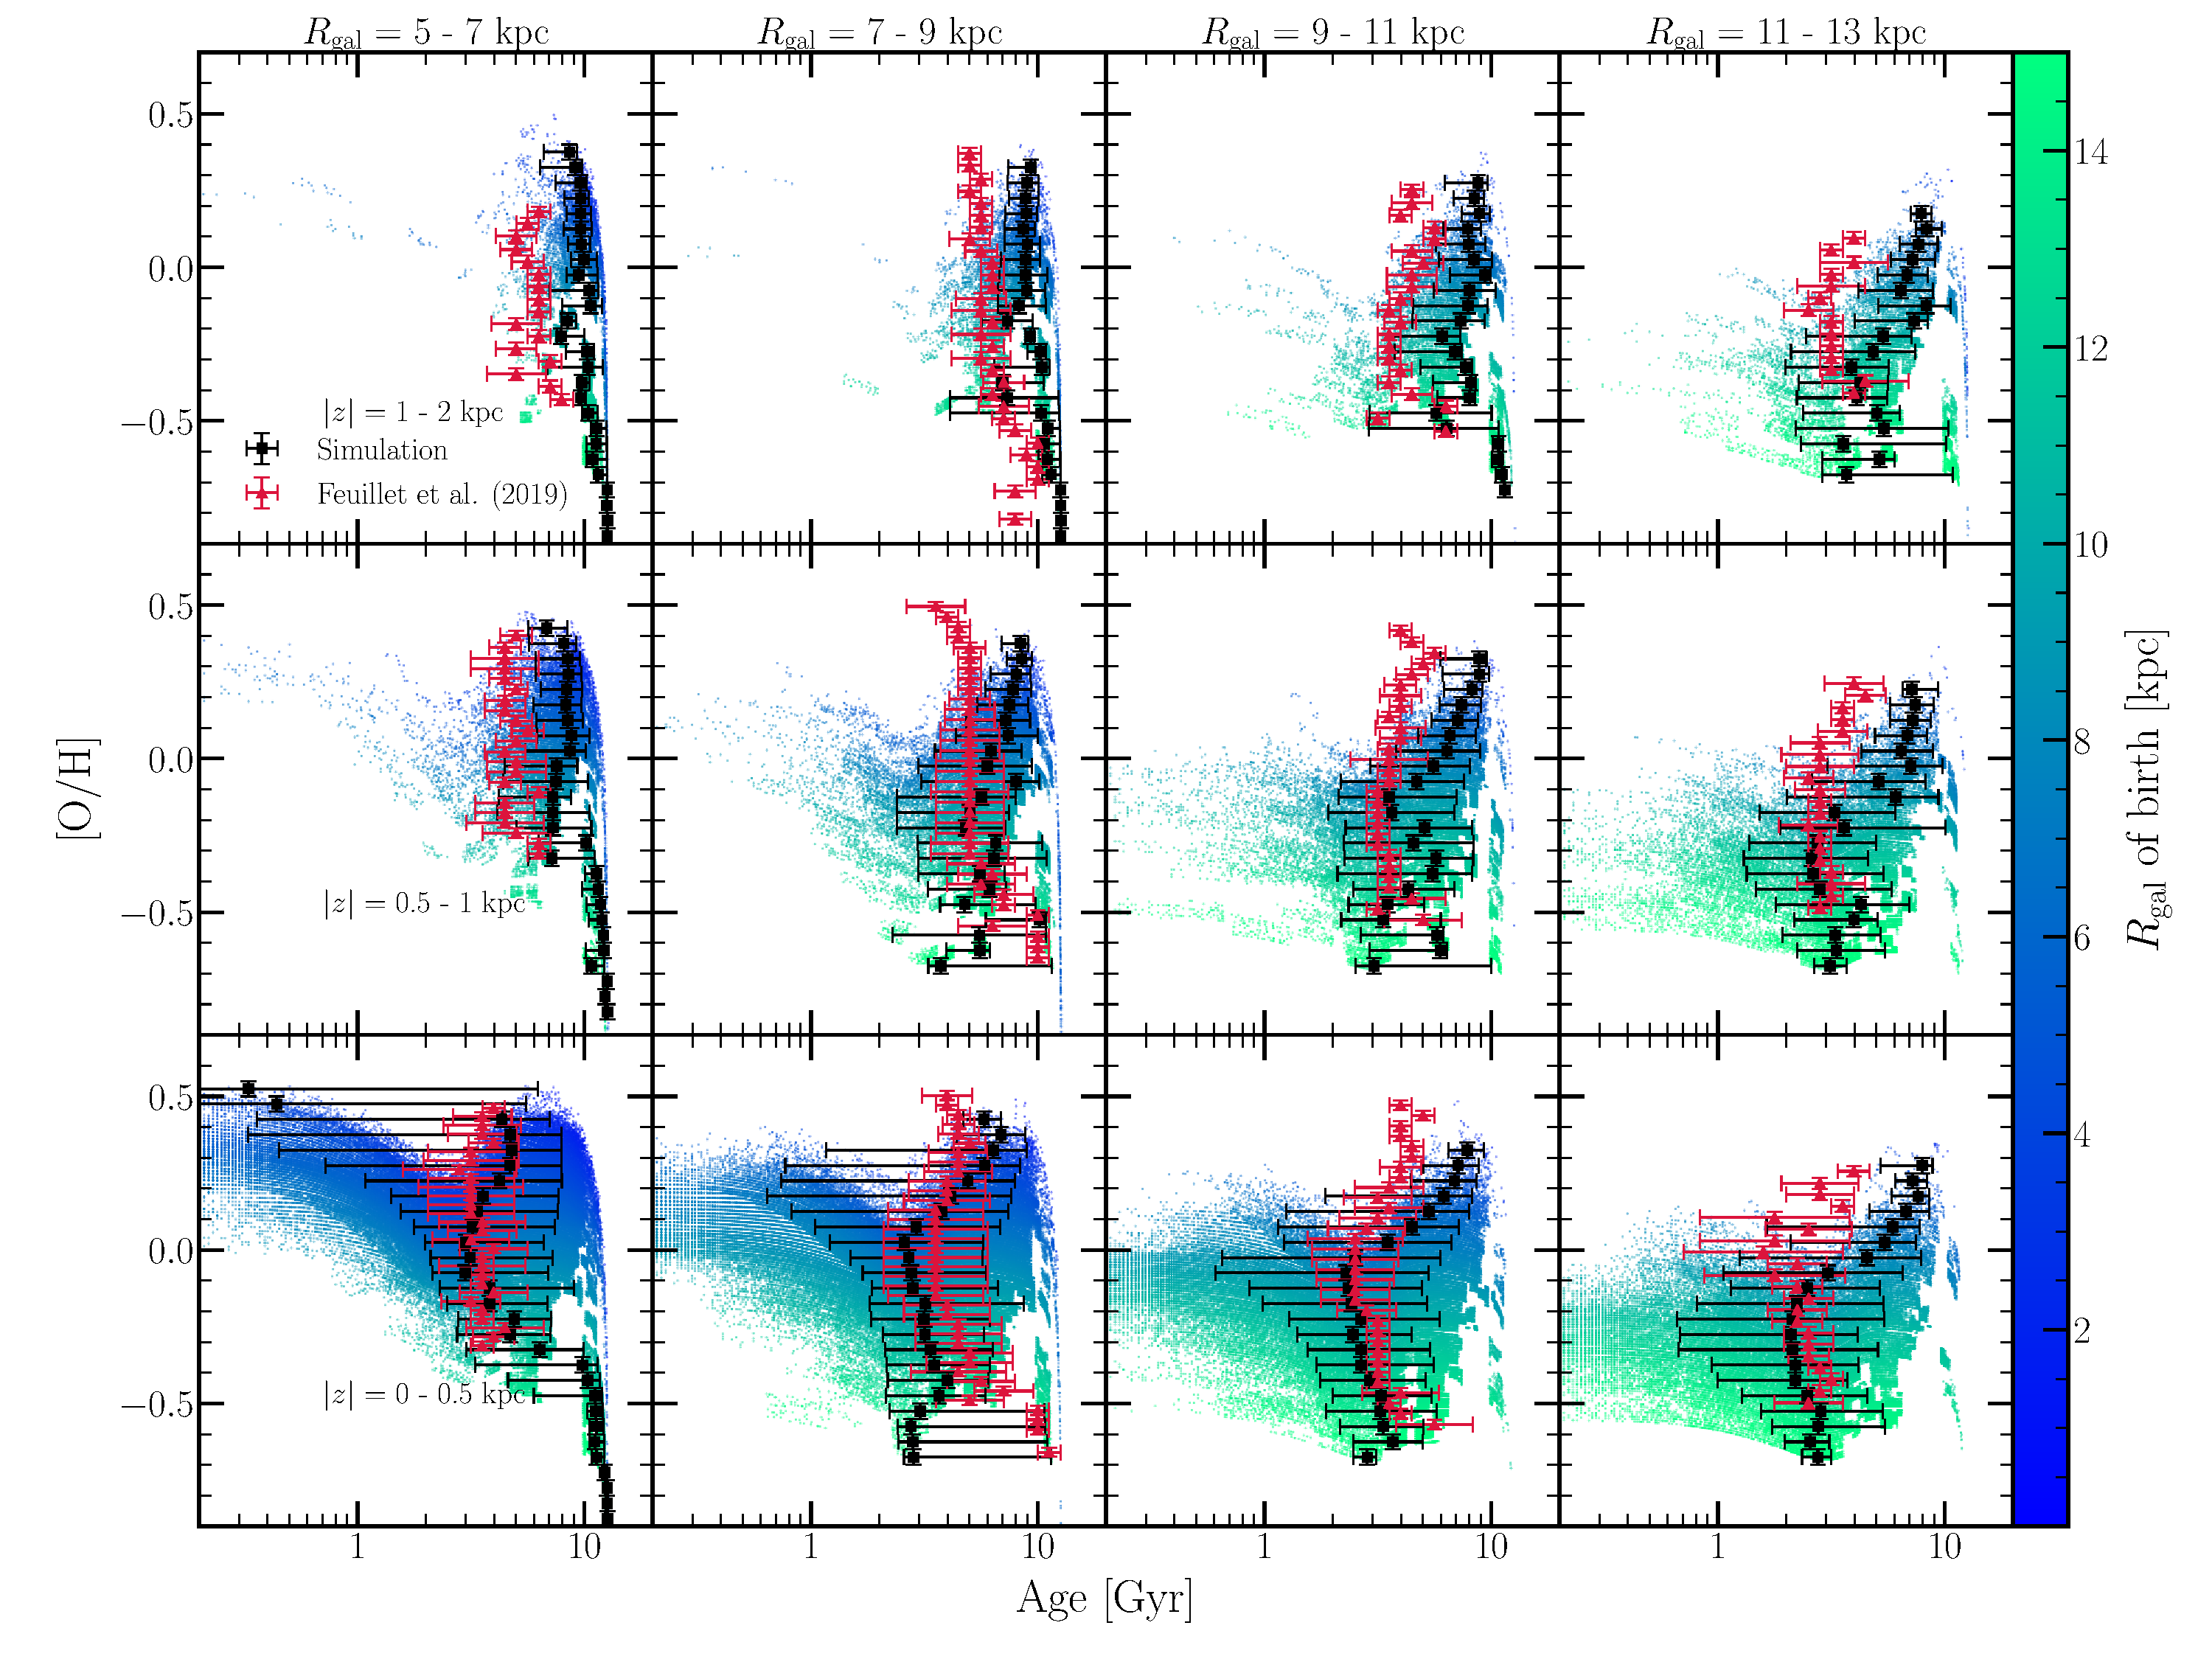
\includegraphics[scale = 0.32]{amr_lateburst_O.pdf} 
\caption{The same as Fig.~\ref{fig:age_alpha_regions}, but for the age-[O/H] 
relation, the late-burst rather than the inside-out SFH, and with our binned, 
simulated relation quantified in 0.05-dex bins in [O/H]. }
\label{fig:age_oh_regions} 
\end{figure*} 

\begin{figure*} 
\centering 
\includegraphics[scale = 0.32]{amr_lateburst_Fe.pdf} 
\caption{The same as Fig.~\ref{fig:age_alpha_regions}, but for the age-[Fe/H] 
relation, the late-burst rather than the inside-out SFH, and with our binned, 
simulated relation quantified in 0.05-dex bins in [Fe/H]. } 
\label{fig:age_feh_regions} 
\end{figure*} 

\begin{itemize} 
	\item Fig.~\ref{fig:age_oh_regions} shows the predicted age-[O/H] relation 
	in 12 Galactic regions from the late-burst SFH in comparison to 
	the~\citet{Feuillet2019} data. Fig.~\ref{fig:age_feh_regions} shows the 
	same thing, but for the age-[Fe/H] relation. 

	\item With increasing $\left|z\right|$, the age distribution of stellar 
	populations moves quickly to high ages, in qualitative agreement with 
	observations. 

	\item Off the midplane, ages are in general overestimated at nearly all 
	radii in both O and Fe, particularly for the $\left|z\right|$ = 1 - 2 kpc 
	regions. 

	\item Find similar results for our other models. What could be causing this 
	discrepancy with the observations? 
	\begin{itemize} 
		\item We assumed that the disk is vertically and azimuthally well-mixed. 
		Could this point to a breakdown in the assumption of efficient vertical 
		mixing? 

		\item The dynamical history of our model is not the Milky Way's 
		dynamical history; it's~\texttt{h277}'s dynamical history. Perhaps the 
		Milky Way had a dynamical disturbance to the disk that kicked a bunch 
		of younger stars to high $\left|z\right|_\text{max}$ orbits (e.g. 
		potentially the Sagitarrius Stream). 
	\end{itemize} 
\end{itemize} 

\section{Metallicity Distribution Functions} 
\label{sec:mdfs} 

\begin{figure} 
\centering 
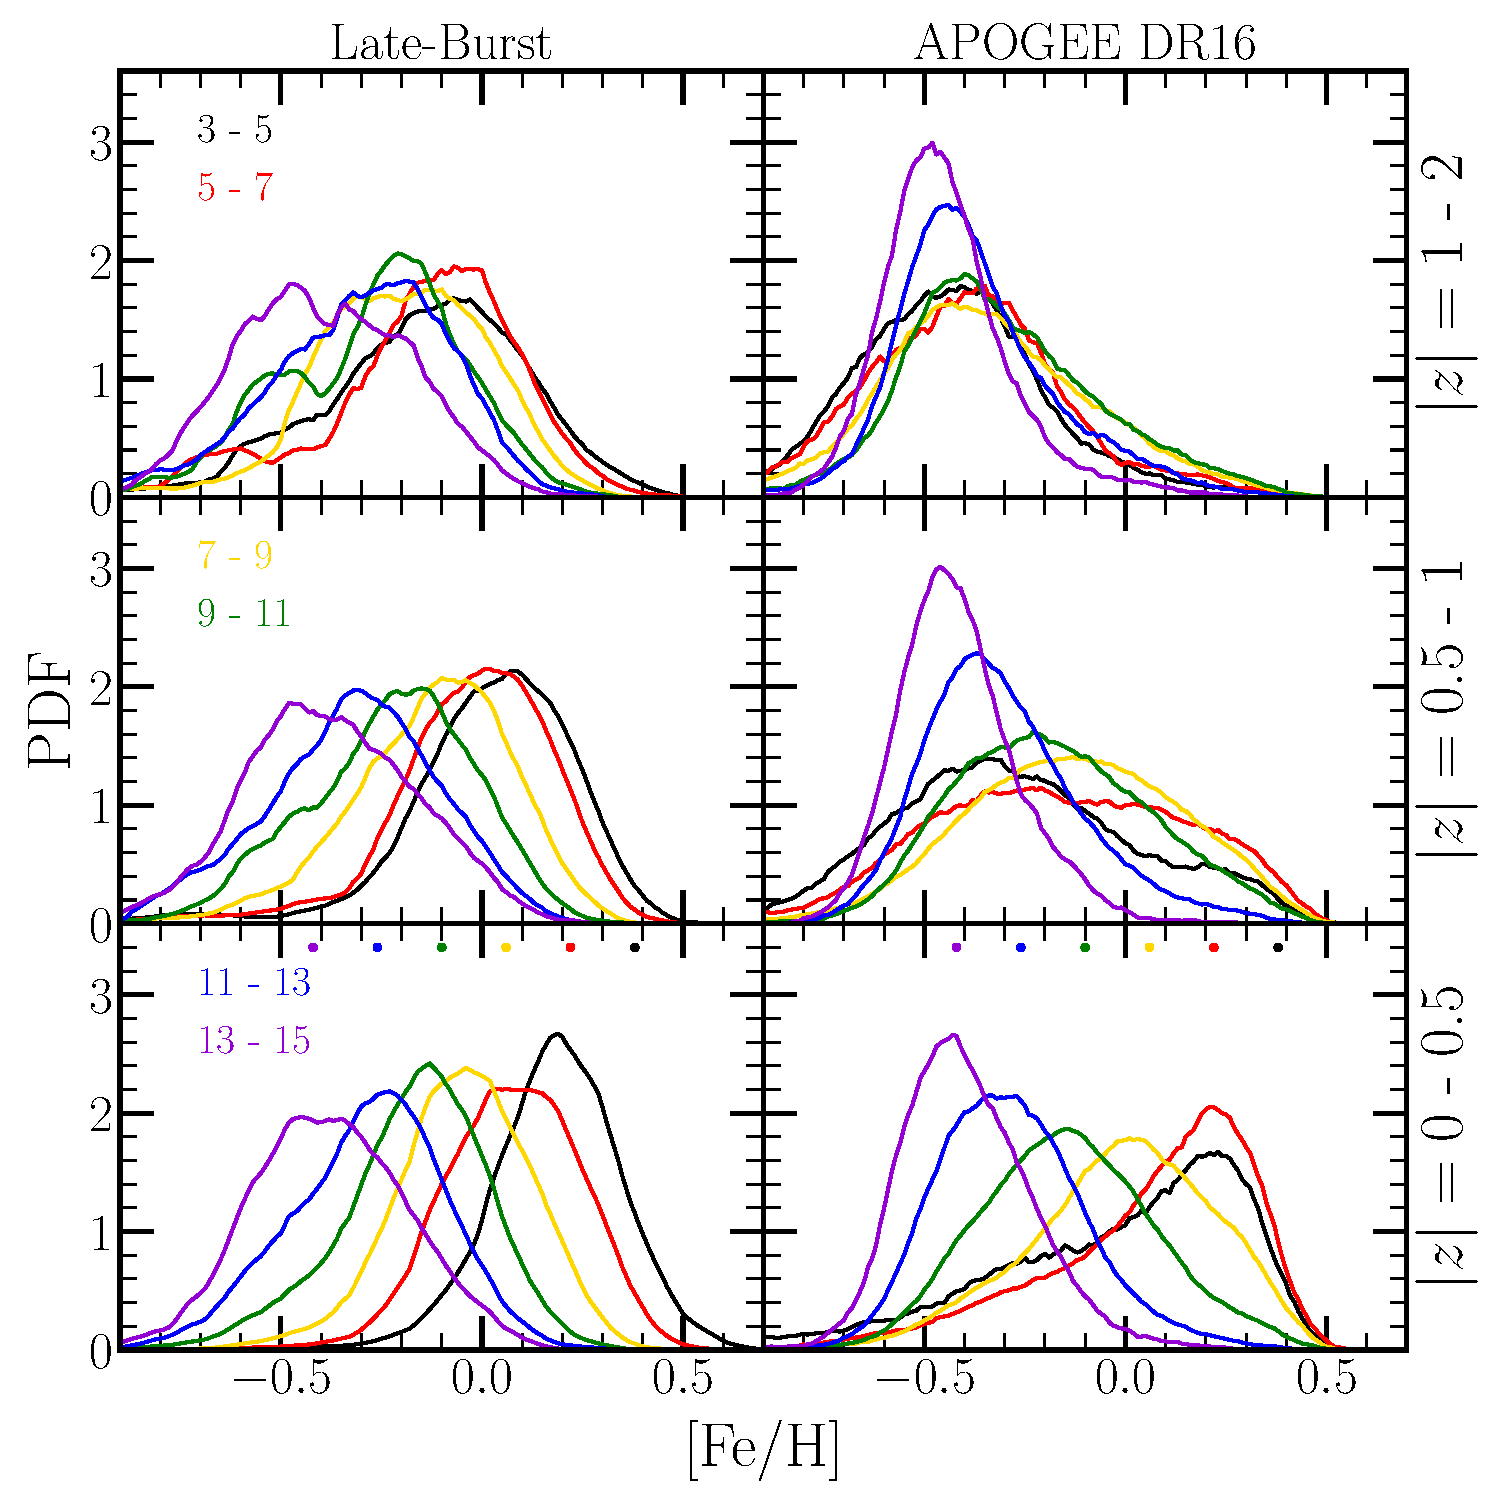
\includegraphics[scale = 0.34]{mdf_3panel_lateburst_Fe.pdf} 
\caption{Metallicity Distribution Functions in [Fe/H] predicted by our 
late-burst model (left) and as observed in APOGEE DR16 (right), for stars and 
simulated stellar populations with present day $\left|z\right|$ = 0 - 0.5 kpc 
(bottom), 0.5 - 1 kpc (middle), and 1 - 2 kpc (top). MDFs are shown in bins 
of Galactocentric radius: 3 - 5 kpc (black), 5 - 7 kpc (red), 7 - 9 kpc 
(yellow), 9 - 11 kpc (green), 11 - 13 kpc (blue), and 13 - 15 kpc (purple). 
The points near the top of the bottom panels denote what the mode abundance 
would be if it followed our target gradient of [Fe/H] = +0.3 at $R_\text{gal}$ 
= 4 kpc and a slope of -0.08 kpc$^{-1}$, assuming the inner radius of each bin 
(i.e. there is no point plotted for 15 kpc). All distributions are smoothed 
with a box-car width of [Fe/H]~$\pm$~0.1. } 
\label{fig:mdf_3panel_fe} 
\end{figure} 

\begin{figure} 
\centering 
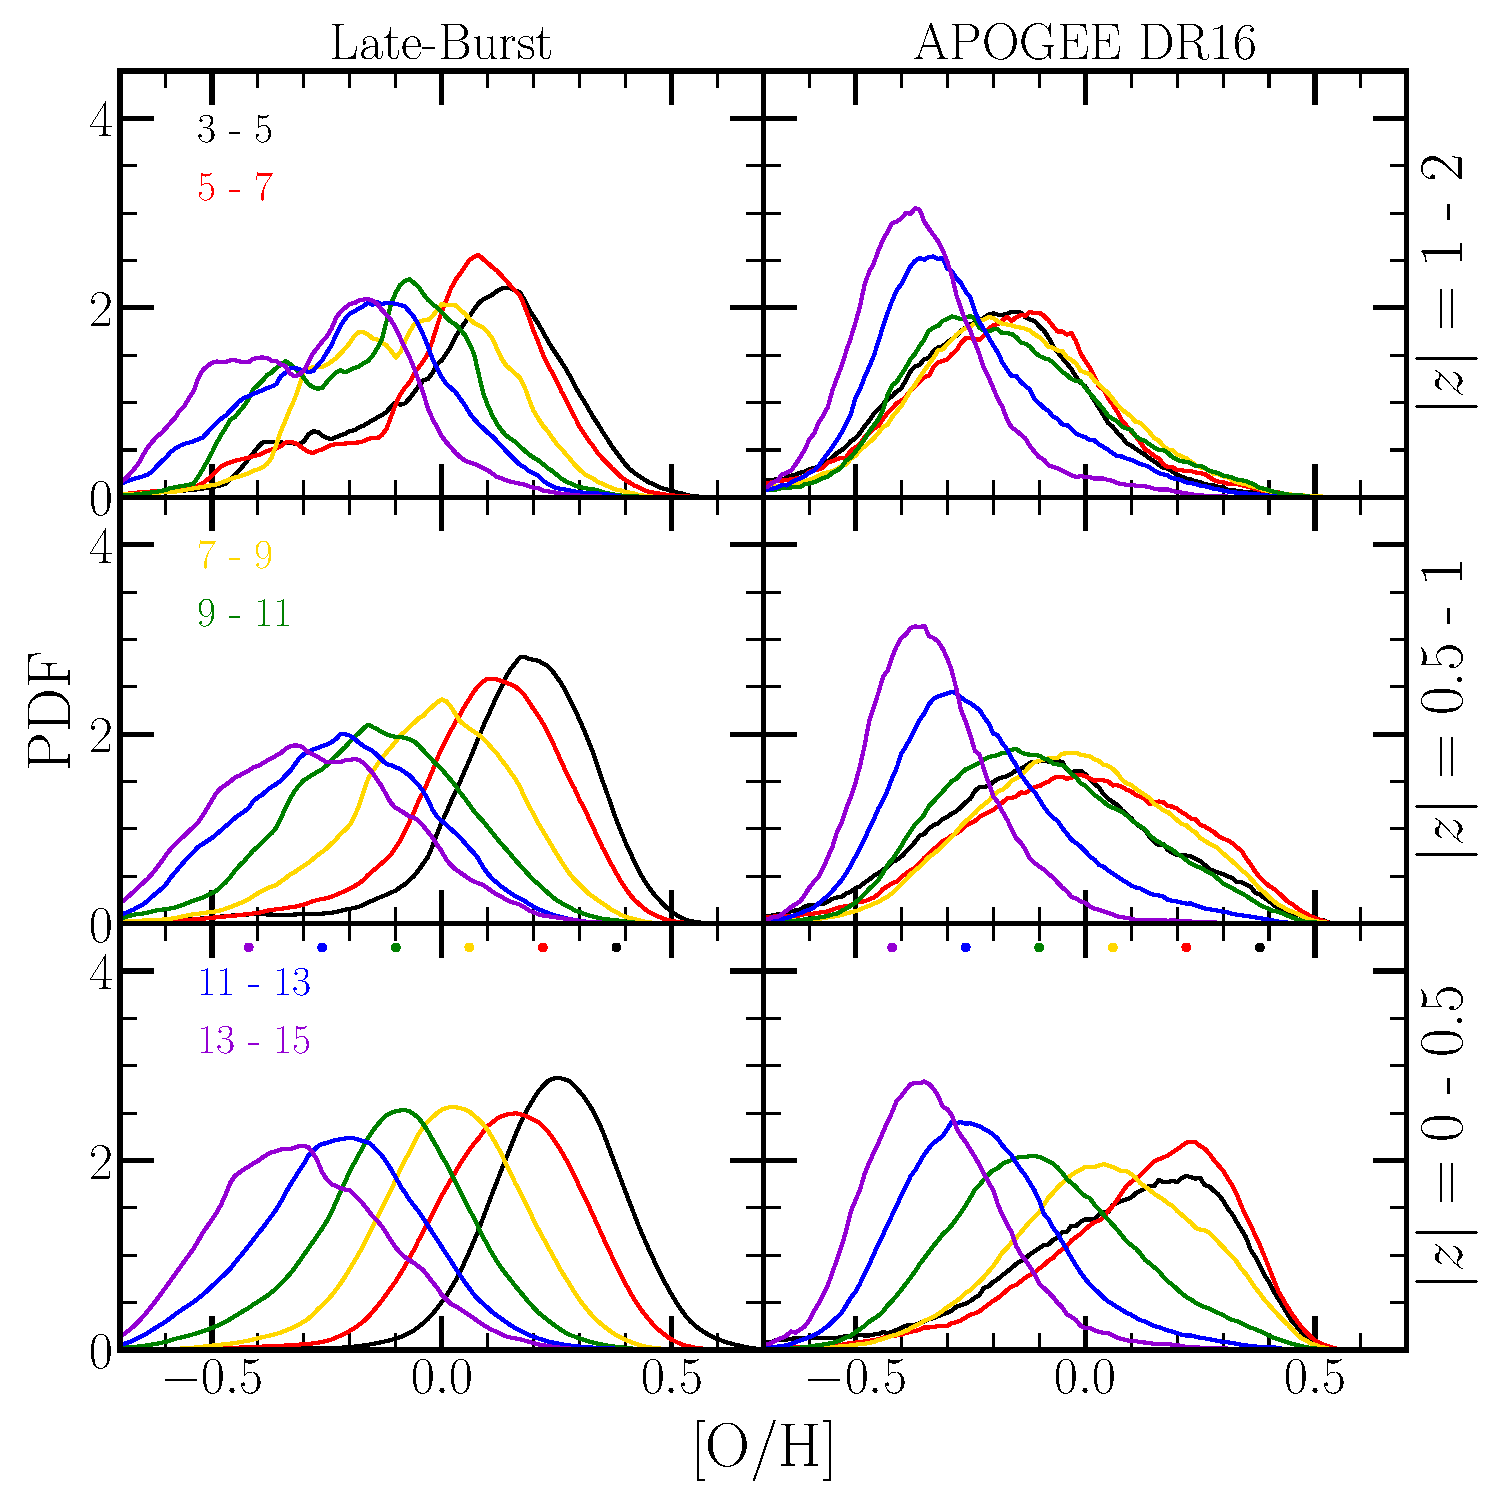
\includegraphics[scale = 0.34]{mdf_3panel_lateburst_O.pdf} 
\caption{The same as Fig.~\ref{fig:mdf_3panel_fe}, but for [O/H].} 
\label{fig:mdf_3panel_o} 
\end{figure} 

\begin{figure*} 
\centering 
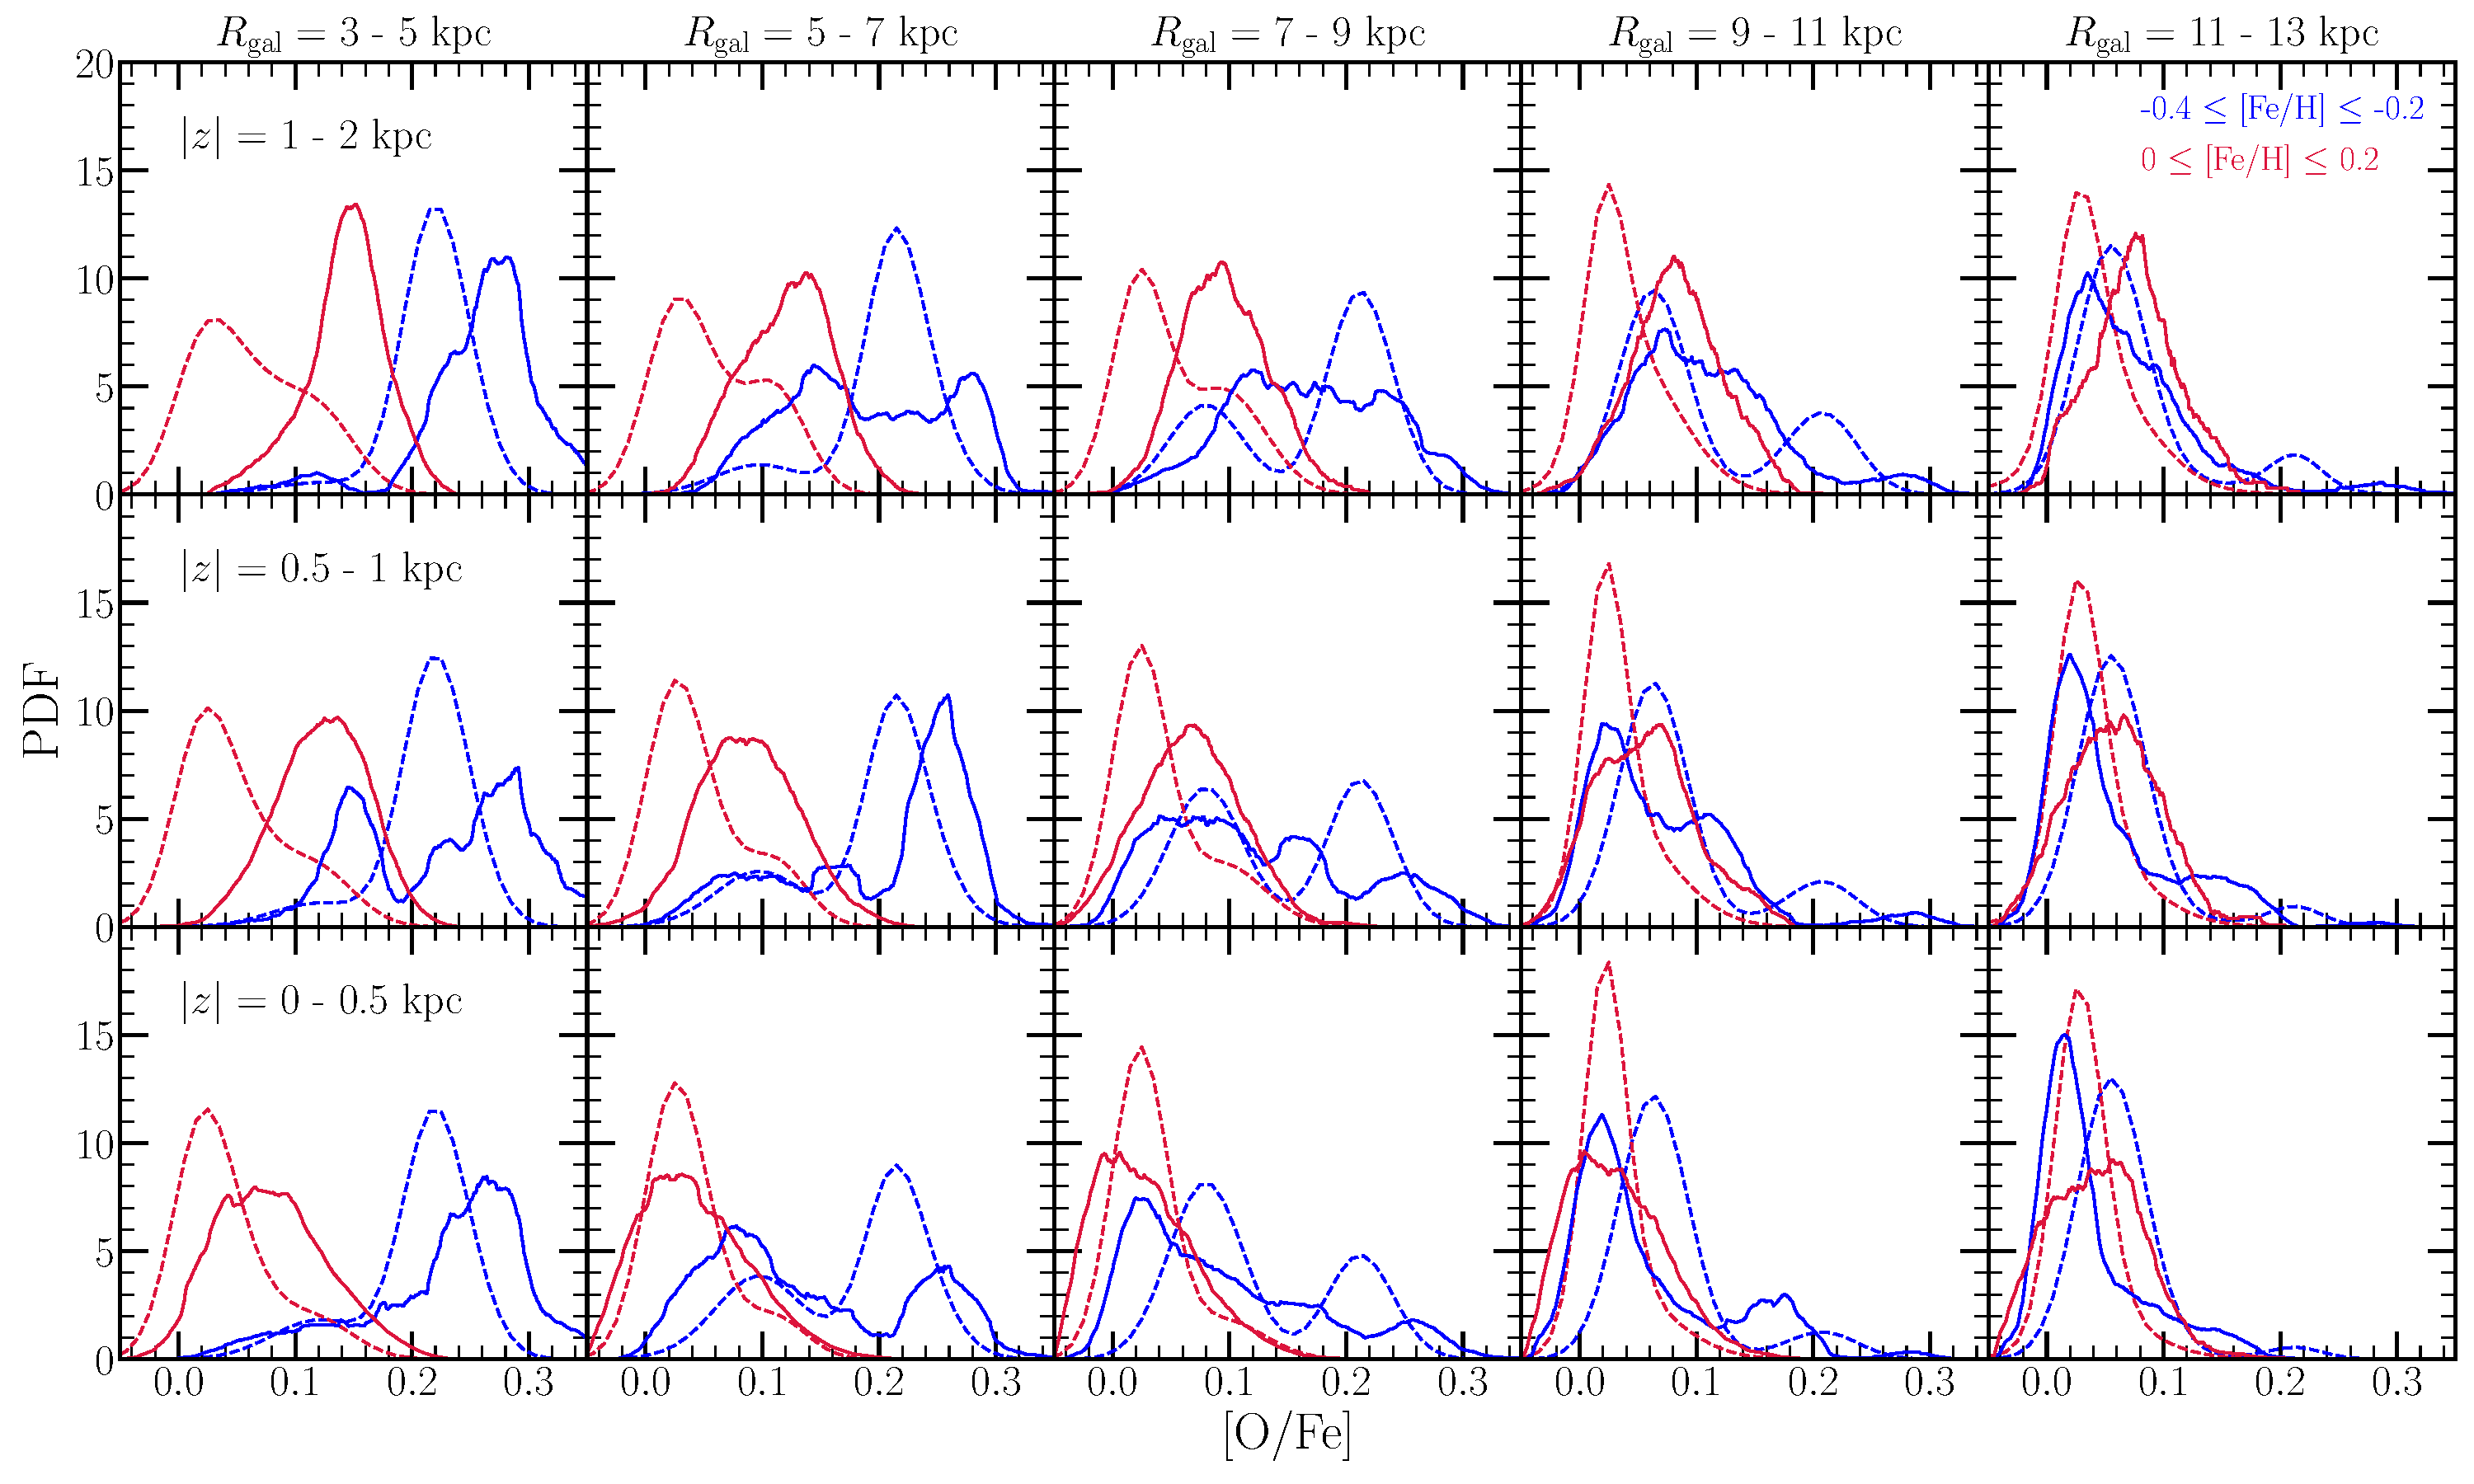
\includegraphics[scale = 0.32]{ofe_mdfs_insideout.pdf} 
\caption{Predicted distributions in [O/Fe] in 15 Galactic regions and in two 
bins in [Fe/H]. Columns correspond to bins in~$R_\text{gal}$, denoted at the 
top of each column. Rows correspond to bins in~$\left|z\right|$, denoted in 
text in the left-hand column. Distributions are color-coded according to the 
[Fe/H] the sample is drawn from, denoted by the legend in the upper right 
panel. Solid lines denote that predicted by our inside-out SFH, while dashed 
lines denote the observed distributions from APOGEE DR16, quantified in 
Vincenzo et al. (2021, in prep). 
\label{fig:ofe_mdfs_insideout} 
}
\end{figure*} 

\begin{figure*} 
\centering 
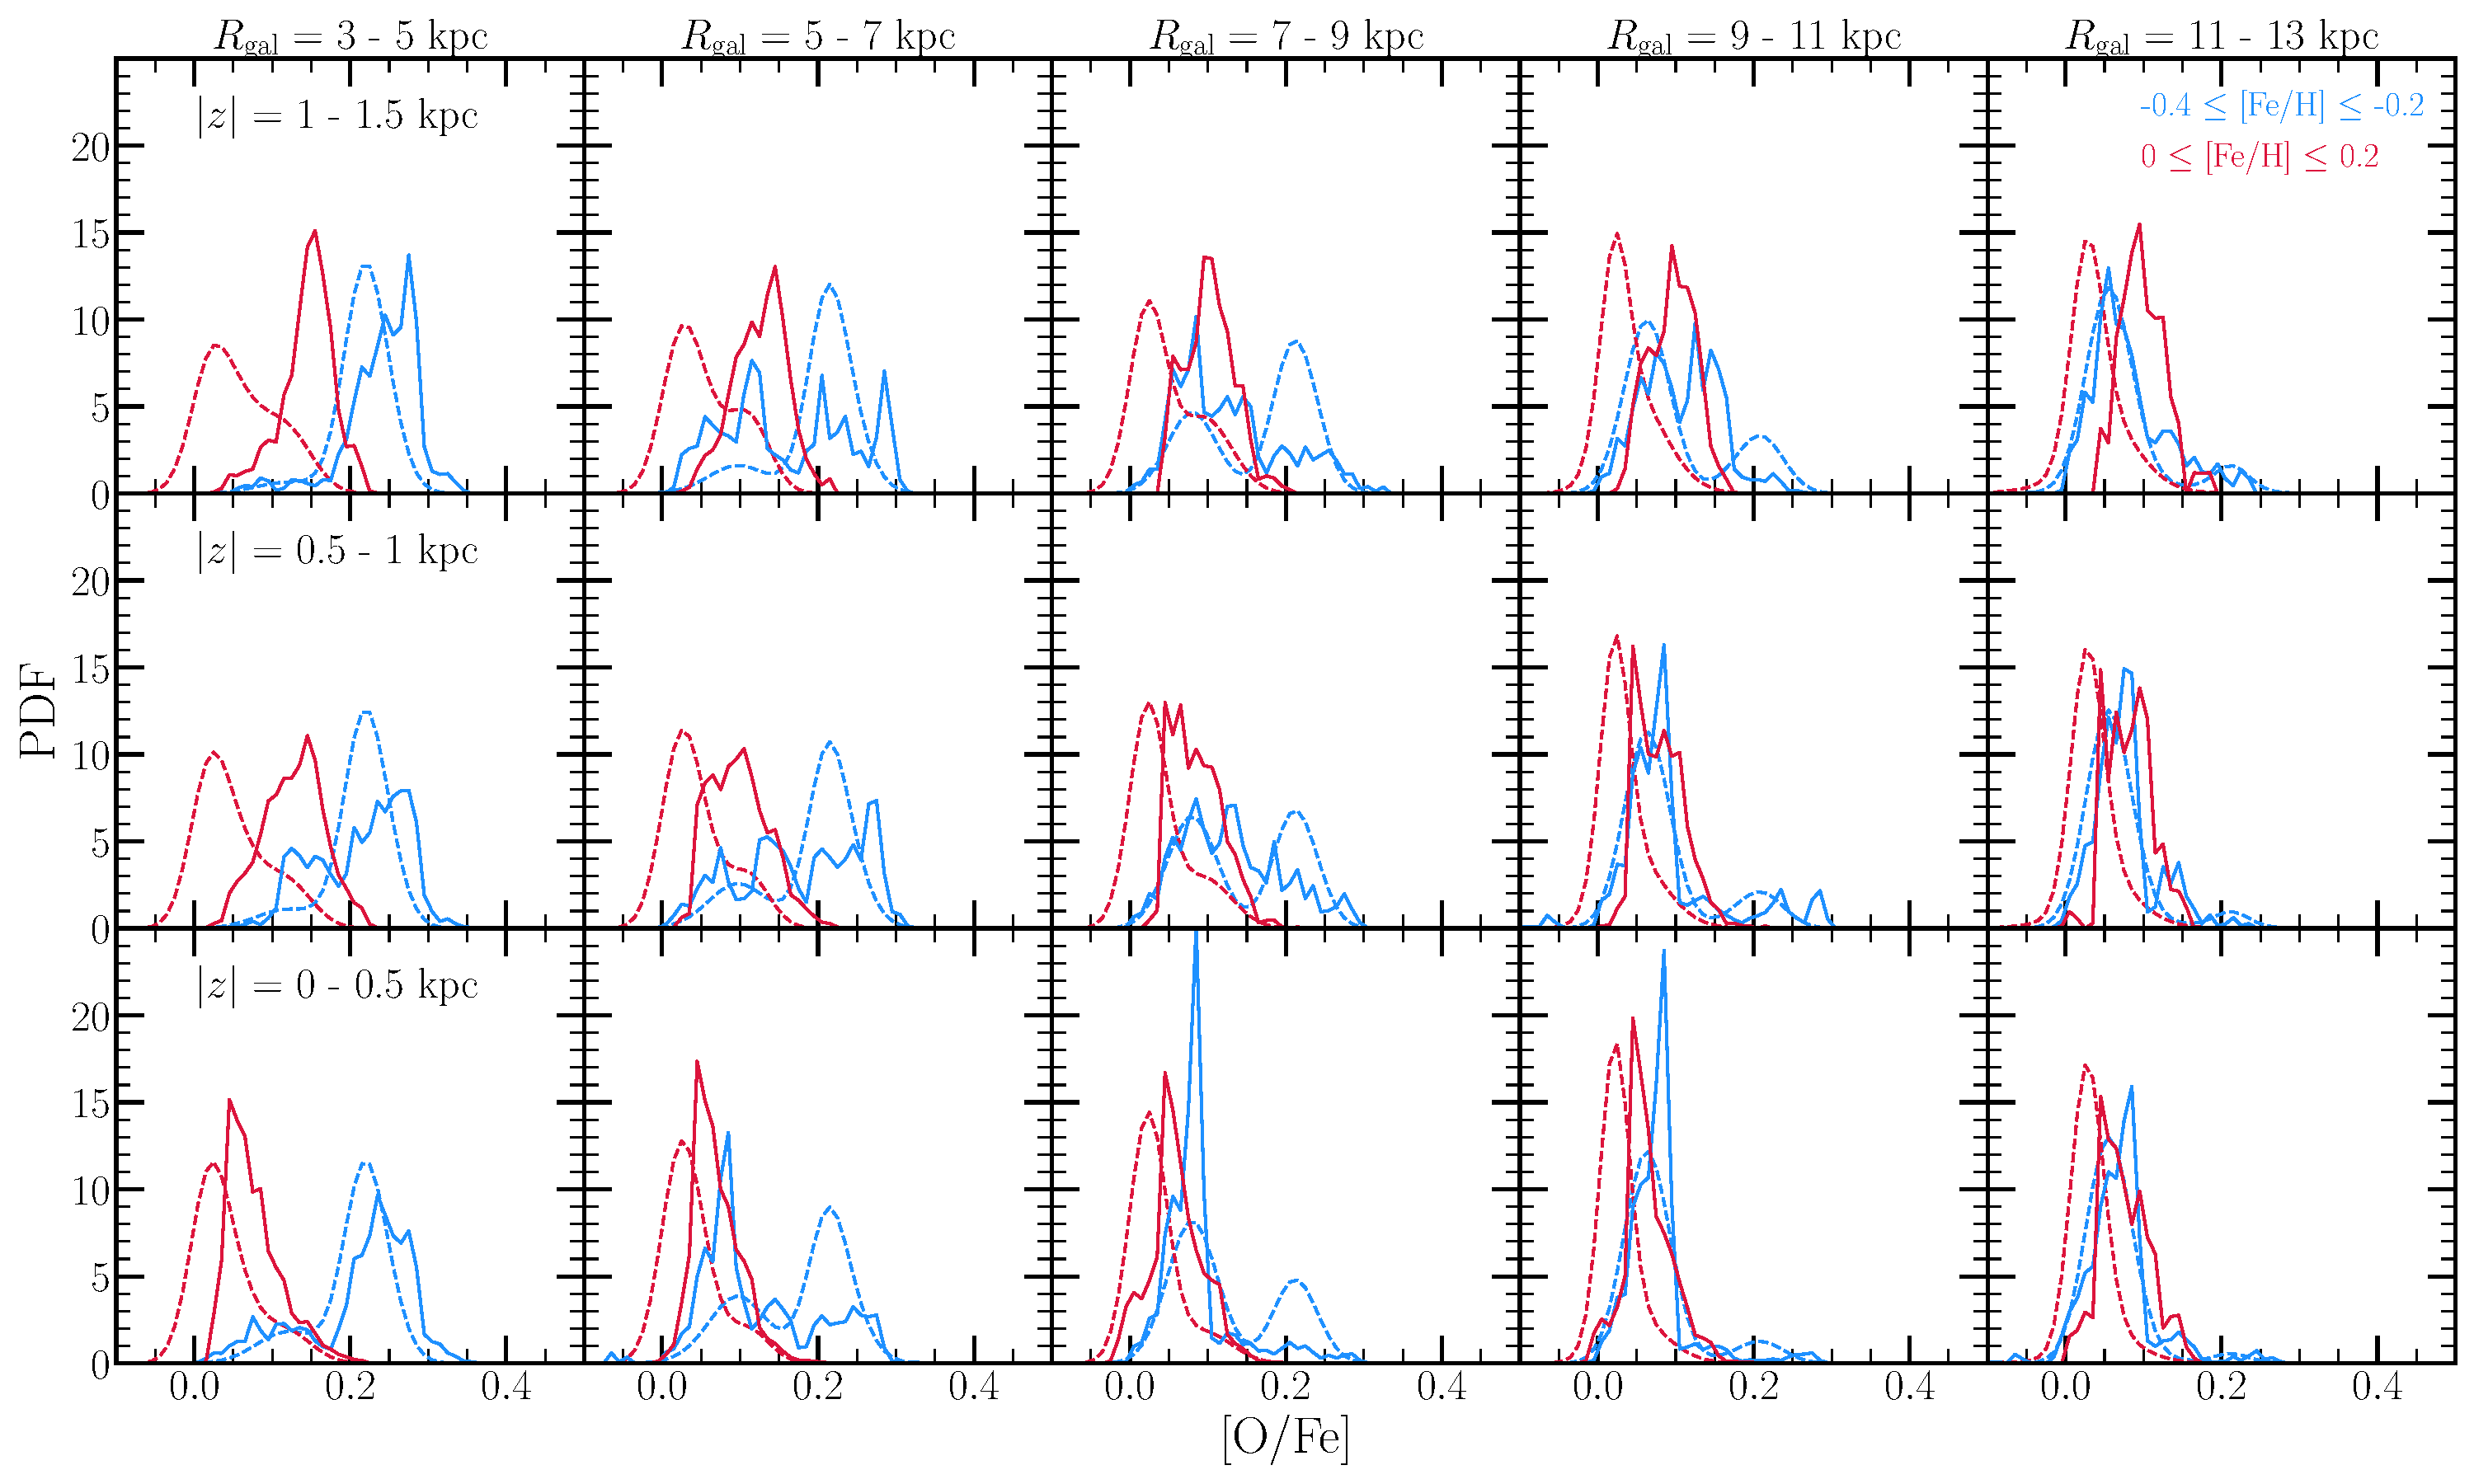
\includegraphics[scale = 0.32]{ofe_mdfs_lateburst.pdf} 
\caption{The same as Fig.~\ref{fig:ofe_mdfs_insideout}, but with the solid 
lines denoting the predictions of our late-burst SFH. } 
\label{fig:ofe_mdfs_lateburst} 
\end{figure*} 

\subsection{[O/H] and [Fe/H]} 
\label{sec:mdfs:oh_feh} 

\begin{itemize} 
	\item MDFs in bins of Galactocentric radius are a fundamental observable 
	to test the validity of any chemical evolution model. 

	\item Previously known that the MDFs in the disk midplane as observed in 
	APOGEE show mode [$\alpha$/H] and [Fe/H] abundances that depend on 
	Galactocentric radius, with a skew-negative distribution in the inner 
	Galaxy and a skew-positive distribution in the outer Galaxy. Off the 
	midplane, the MDFs merge and converge on [$\alpha$/H]~$\approx$~[Fe/H] 
	$\approx$~-0.5~\citep{Hayden2015, Weinberg2019}. This result is replicated 
	in the left-hand column of panels in Fig.~\ref{fig:mdf_3panel_fe} and 
	Fig.~\ref{fig:mdf_3panel_o}. 
	\begin{itemize} 
		\item Similar mode [O/H] and [Fe/H] between the 3 - 5 and 5 - 7 kpc in 
		the APOGEE observations. What could be the origin of this? Cessation of 
		star formation in the inner Galaxy? (see Fig. 1 of~\citealp{Peek2009} 
		and Fig. 2 of~\citealp{Fraternali2012}). This would imply very few 
		stars formed in the most metal-rich regions of the Galaxy, cutting off 
		the MDF at high [O/H], [Fe/H]. 
	\end{itemize} 

	\item Left-hand panels of Figs.~\ref{fig:mdf_3panel_fe} 
	and~\ref{fig:mdf_3panel_o} show the distributions predicted by our 
	late-burst model. They successfully replicate the qualitative result that 
	the mode [X/H] varies with present-day Galactocentric radius, but fail to 
	show a similar mode abundance between the 3 - 5 and 5 - 7 kpc bins. 
	Potentially linked to the cessation of star formation in inner 
	Galaxy~\citep{Peek2009, Fraternali2012}. 

	\item Beyond the midplane, our models fail to fully replicate the 
	convergence of the MDFs at [x/H]~$\approx$~-0.5. The observed MDF at small 
	radii shifts from skew-negative with a metal-rich mode to skew-positive 
	with a metal-poor mode with increasing $\left|z\right|$. In our predicted 
	MDFs for the inner galaxy, the mode does shift to lower [X/H], though not 
	as low as in the observations. There is also very little change in 
	skewness with $\left|z\right|$ predicted, in tension with observations. 
	\begin{itemize} 
		\item Could this point to a breakdown of our assumption that vertical 
		mixing is efficient? 

		\item Some discussion in~\S~\ref{sec:amr} that the Sagitarrius stream 
		may be responsible for the young ages observed at high~$\left|z\right|$ 
		in~\citet{Feuillet2019}. This likely wouldn't solve the problem here, 
		because our annuli are at or near equilibrium at the lookback times 
		associated with the Sagitarrius dwarf's pericentric passages, meaning 
		this effect would only kick high [X/H] stars to high~$\left|z\right|$. 
	\end{itemize} 

	\item We note that our models do a good job of producing a mode [X/H] 
	abundance in each radial bin close to our target gradient. In the inner 
	galaxy bins in Figs.~\ref{fig:mdf_3panel_fe} and~\ref{fig:mdf_3panel_o}, 
	the predicted mode is moderately lower than the target, but this is due 
	to the effect of dilution (see discussion in~\S~\ref{sec:amr}). In our 
	inside-out model, the difference in target and predicted mode [X/H] is 
	considerably smaller. 
\end{itemize} 

\subsection{[O/Fe]} 
\label{sec:mdfs:ofe} 

\begin{itemize} 
	\item Fig.~\ref{fig:ofe_mdfs_insideout} show distributions in [O/Fe] in two 
	bins of [Fe/H] across 15 Galactic regions predicted by our inside-out SFH 
	(solid lines). 

	\item Dashed lines denote the distributions quantified in Vincenzo et al. 
	(2021, in prep). These are intended to simultaneously remove the effects of 
	observational errors in [O/Fe] and the APOGEE selection function in these 
	Galactic regions; that is, these are estimates of the~\textit{intrinsic} 
	[O/Fe] distributions that, when convolved with observational uncertainties 
	and the APOGEE selection function, would resemble the observed MDFs. 

	\item We note that the inside-out model fails to reproduce a Milky Way-like 
	bimodality. Such a model prediction would appear as good agreement between 
	the solid and dashed lines in Fig.~\ref{fig:ofe_mdfs_insideout}, but that 
	is not the case. There may be decent agreement in a given metallicity bin 
	and Galactic region, but the agreement would need to be seen everywhere and 
	at all metallicities. 

	\item In the inner galaxy, we overestimate the [O/Fe] of the highest [Fe/H] 
	stars at all $\left|z\right|$, and the differences in the distributions 
	gets smaller with increasing~$R_\text{gal}$. The lower [Fe/H] bins don't 
	seem to have this problem. 
	\begin{itemize} 
		\item Since these are in specific bins in [Fe/H], this is an indication 
		that our model is overpredicting the O abundances of these stars, 
		rather than underpredicting [Fe/H]. 

		\item This could point to various things. Perhaps the Milky Way has 
		different gradients in [O/H] than [Fe/H], an effect which is not 
		captured by these models. Perhaps the innermost radii of the Milky Way 
		has some contamination from bulge stars, another effect which is not 
		captured by our models. 
	\end{itemize} 

	\item Fig.~\ref{fig:ofe_mdfs_lateburst} shows the same thing as 
	Fig.~\ref{fig:ofe_mdfs_insideout}, but for the late-burst SFH. 

	\item We note that this model does not predict a Milky Way-like bimodality 
	either, and still suffers from the issues facing the inside-out model 
	regarding the highest [Fe/H] stars in the inner Galaxy. 

	\item While the notion that an [$\alpha$/Fe] dichotomy can arise out of 
	radial migration alone was put forth in~\citet{Schoenrich2009}, this 
	suggests that an inside-out star formation history combined with stellar 
	migration is not conducive to predicting this observed result. This is at 
	odds with the findings of~\citet{Sharma2020}, who claim to reproduce the 
	[$\alpha$/Fe] dichotomy with an analytic chemical evolution model. 
	\begin{itemize} 
		\item {\color{red} We'll need to be careful in our final draft of the 
		paper so that our language here isn't too strong. Below I've given my 
		honest critiques of the~\citet{Sharma2020} paper. } 

		\item They have a single SFH. 

		\item They assume a functional form for [Fe/H] and [$\alpha$/Fe] with 
		time and radius, indicating that their [$\alpha$/Fe]-[Fe/H] tracks are 
		\textit{not} model predictions, and are instead assumptions 
		characterized~\textit{a priori} by radius and time. Rather than 
		learning about the physical origins of the [$\alpha$/Fe] dichotomy, we 
		instead get a robust mathematical caricature of the data. 

		\item They find a dichotomy in the [$\alpha$/Fe]-[Fe/H] plane to arise 
		out of a fast transition in the gas phase between high-$\alpha$ and 
		low-$\alpha$. In practice, we find that this is only the case if 
		$\tau_\star$ is sufficiently short; analytic justification for this is 
		also presented in~\citet{Weinberg2019} ({\color{red} We could 
		potentially demonstrate this in Appendix~\ref{sec:sfe_variations} as 
		well}). In this paper, we adopted the~\citet{Tacconi2018} scaling of 
		$\tau_\star^\text{mol}$ with redshift. We find that none of our models 
		predict a~$\tau_\star$ adequately short such as to produce an 
		adequately fast transition between high-$\alpha$ and low-$\alpha$ 
		sequences, as assumed in the~\citet{Sharma2020} analysis. 

		\item For these reasons, we believe our investigation to be more robust, 
		physically motivated, and internally consistent than 
		the~\citet{Sharma2020} analysis. 
	\end{itemize} 

	\item These findings suggest that an inside-out SFH combined with radial 
	migration, even when a late starburst is taken into account (as motivated 
	by the findings of~\citealp{Isern2019} and~\citealp{Mor2019}), 
	is~\textit{not} conducive to producing the observed [$\alpha$/Fe] 
	dichotomy. This suggests that more dramatic evolutionary events are likely 
	responsible, such as a two-infall model~\citep[e.g.][]{Chiappini1997, 
	Chiappini2001, Romano2010, Grisoni2017, Noguchi2018, Spitoni2009, 
	Spitoni2016, Spitoni2018, Spitoni2019, Spitoni2020}. 
\end{itemize} 

\section{Conclusions} 
\label{sec:conclusions} 
\begin{itemize} 
	\item We have modeled the Milky Way as a series of concentric annuli with 
	$\Delta R_\text{gal}$ = 100 pc width. We investigated a handful of 
	assumptions about the SFH, the time-dependence of radial migration, and 
	star formation efficiency, and a multitude of combinations thereof under 
	a simulation-based model for stellar migration independent of free 
	parameters. 

	\item We found that similar numbers of star particles in~\texttt{h277} 
	migrated inward as outward, and that the two proceed on different 
	timescales, indicating that they're potentially linked to different 
	physical processes. 

	\item We found that the e-folding timescales for star formation indicated 
	by population averaged observations of Milky Way like galaxies are long 
	($\sim$15 Gyr in the solar annulus;~\citealp{Sanchez2020}). 

	\item We found that our recipe for setting the gradients in both stellar 
	surface density and metallicity yields the correct result. This is an 
	indication that radial migration does not change the profile of these 
	observed trends, only inducing scatter. 
	\begin{itemize} 
		\item We found that slightly different predictions in the stellar 
		and gas-phase metallicity gradient are natural consequences of 
		variations in the SFH. 

		\item We found that different models for the SFH predicted different 
		[O/Fe] gradients at the present day. 
	\end{itemize} 

	\item We found that the time-dependence of radial migration indeed does 
	have an impact on enrichment. Previous studies in the literature have 
	assumed that this is not the case, due to the slow nature of migration 
	\citep[e.g.][]{Minchev2013}. However, we find that even for young stars, 
	the tails of the present-day $R_\text{gal}$ distribution are adequately 
	long that when age-dependent migration is taken into account, the model 
	predicts variations in the SN Ia rate that then impact predicted abundance 
	ratios. We demonstrated that this is a means with which stellar migration 
	may produce young, Fe-poor stars which can migrate to the solar annulus, 
	and potentially be misinterpreted as young, $\alpha$-rich stars. This is 
	proof of concept that the radial migration of nucleosynthetic yields can 
	proceed alongside the radial migration of stars, depending on which model 
	for migration that you believe. 
	\begin{itemize} 
		\item These stars have been seen in observed data from APOGEE 
		\citep[e.g.][]{SilvaAguirre2018}. They postulate that since these stars 
		have kinematics similar to the rest of the high-$\alpha$ population, 
		that perhaps they are the consequence of stellar mergers or mass 
		transfer events, producing truly old stars that simply appear to be 
		younger. While these interpretations are not mutually exclusive, an 
		observational test to ascertain the origins of the observed young 
		$\alpha$-rich population would have implications for which of the 
		models for radial migration investigated here are the most realistic. 
	\end{itemize} 

	\item In the observations, the high-$\alpha$ sequence is known to be most 
	prominent at low~$R_\text{gal}$ and high~$\left|z\right|$, and conversely, 
	the low-$\alpha$ population at high~$R_\text{gal}$ and low~$\left|z\right|$ 
	\citep[e.g.][]{Hayden2015}.  We found that this is a natural consequence of 
	stellar migration, though the detailed distributions depend on the SFH and 
	the relative yields of $\alpha$ and iron-peak elements, both of which are 
	highly uncertain, and we do not model them in detail here. 

	\item We found that our inside-out model predicts an age-[$\alpha$/Fe] 
	relation which is in good agreement with the observed relation reported 
	by~\citet{Feuillet2019}. Our recent starburst models predict a global 
	$\alpha$-enhancement that simply isn't seen in the data. This suggests 
	that our current understanding of chemical evolution may be at odds with 
	the findings of~\citet{Mor2019} and~\citet{Isern2019} suggesting a recent 
	factor of~$\sim$2 enhancement in the Milky Way SFH peaking~$\sim$2 Gyr ago. 

	\item We find that where our inside-out SFH model fails to agree with the 
	age-[O/Fe] relation reported by~\citet{Feuillet2019}, it tends to 
	overpredict ages at a given [O/Fe]. However, it tends to fail in a manner 
	such that the~\citet{Feuillet2019} relation agrees with the stars that we 
	would call Fe-poor - that is, the stars that are $\alpha$-enhanced due to 
	forming out of an Fe-poor ISM due to the same variations in the SN Ia rate 
	that can produce young, $\alpha$-rich stars. While this may be coincidence, 
	if we take the observations at face value, it would suggest that our model 
	is overpredicting the rate of Fe injection, and that perhaps SN Ia yields 
	of Fe should be lower. If we take the model at face value, it suggests that 
	APOGEE+Gaia targets preferentially sample young, $\alpha$-rich stars 
	(\citealp{Feuillet2019} used APOGEE data for stars with Gaia parallaxes). 

	\item We found that the age-metallicity relation (AMR) in both [O/H] and 
	[Fe/H] reported by~\citet{Feuillet2019} is better fit by our late 
	starburst models. This is at odds with the findings regarding the 
	age-[O/Fe] relation, where the inside-out model agreed with the data much 
	better than the starburst models. This is interesting, because different 
	observables are favoring different models for the SFH, suggesting that 
	something more complicated is going on. 
	\begin{itemize} 
		\item The starburst models agreeing with the observed AMR has more to 
		do with the effect of dilution than the starburst itself. In trying to 
		model the Milky Way, we might be able to have our cake and eat it too 
		if there were dilution with no ensuing starburst. This could suggest 
		some accretion event that was primarily HI gas that hasn't yet cooled 
		to be available for star formation. 

		\item Off the midplane, our model-predicted AMR overestimates ages 
		relative to~\citet{Feuillet2019}, just like in the age-[O/Fe] relation. 
		We speculate that this may be related to the Sagitarrius dwarf 
		galaxy; it's important to remember that our model galaxy does not have 
		the Milky Way's dynamical history, but~\texttt{h277}'s dynamical 
		history. {\color{red} Jon and I are looking into this, but as I 
		understand it, what I've written next is in general true.}~\texttt{h277} 
		did not have a Sagitarrius-like accretion event. Since Sagitarrius 
		has made multiple pericentric passages nearly head-on with the Milky 
		Way disk, it's possible that young stars were kinematically heated to 
		high~$\left|z\right|$, an effect that would not be present in 
		\texttt{h277} without such an event. This would decrease our model 
		predicted median ages at these heights by directly adding more young 
		stars, and potentially not having noticeable effect in the midplane due 
		to the much larger number of stars there. 
	\end{itemize} 

	\item We find that our models naturally reproduce the variations in the 
	observed metallicity distribution functions (MDFs) with Galactocentric 
	radius. At low~$R_\text{gal}$, the mode abundance in both [O/H] and [Fe/H] 
	is high, and conversely low at high~$R_\text{gal}$. However, our predicted 
	distributions are too narrow, where in the observations the low 
	$R_\text{gal}$ MDF is significantly skew-negative, and conversely 
	skew-positive at high~$R_\text{gal}$~\citep{Hayden2015}. Also in the 
	observed relation, the mode abundance at 3 - 5 kpc is strikingly similar to 
	the mode abundance at 5 - 7 kpc. Our models fail to reproduce this, though 
	it may be tied to a cessation of star formation in the inner galaxy as 
	suggested by~\citet{Peek2009} and~\citet{Fraternali2012}. 

	\item We find that none of our models predict a Milky Way-like dichotomy 
	in [$\alpha$/Fe], as observed by many studies. This suggests that inside-out 
	galaxy growth combined with radial migration, even if a recent starburst 
	is included, is not adequate to explain the observed dichotomy. This is at 
	odds with~\citet{Sharma2020}, though we believe our study to be the more 
	robust. 

	\item \texttt{VICE} is publicly available and open-source. It can be 
	installed via~\texttt{pip} (\url{https://pypi.org/project/vice}). 
	Documentation is available at~\url{https://vice-astro.readthedocs.io}. 
	Source code is hosted at~\url{https://github.com/giganano/VICE.git}. 
\end{itemize} 

\section{Acknowledgements} 
\label{sec:acknowledgements} 
We are grateful to Diane Feuillet for sharing the data 
from~\citet{Feuillet2018} and~\citet{Feuillet2019} with us. {\color{red} There 
will be others added, depending on whether or not they go here or on the 
author's list. I'll also need to add the SDSS acknowledgements since we made 
use of APOGEE data.} 

\section{Data Availability} 
{\color{red} In case anyone hasn't seen one of these Data Availability 
statements yet, this is now a requirement by MNRAS. It wasn't when I submitted 
my last paper, but was by the time we were finished with the referee report, 
so I wound up having to add one. They just want you to say if the data are 
available to the reader or not, and where/how they can get it if they are. }
\texttt{VICE} is open source software, and as such the source code for these 
simulations is publicly available.\footnote{
	\url{https://pypi.org/project/vice} \\ 
	\url{https://vice-astro.readthedocs.io} \\ 
	\url{https://github.com/giganano/VICE.git} 
} The source code which produces the outputs presented in this paper as well as 
the figures are included as secondary material in the GitHub repository. 
While the aggregate of all outputs analyzed in this paper are sufficiently 
large that it is not conducive to store them on GitHub, we provide instructions 
on how to run our simulations and variations thereof. All observational data 
appearing in this paper is publicly available, and is also included with the 
source code for our simulations and figures. 

\newpage 
\begin{appendices} 

\section{Normalizing a Fiducial Star Formation History} 
\label{sec:normalize_sfh} 
\begin{itemize} 
	\item Derive formula for normalizing an SFH given the time-dependence at 
	a given radius $f(t|R_\text{gal})$ and the radial dependence of the 
	desired surface density gradient at late times $g(R_\text{gal})$. Neither 
	need be normalized. 
	\begin{equation} 
	\dot{\Sigma}_\star(R_\text{gal}, t) = \dot{\Sigma}_{\star,0}(R_\text{gal}) 
	f(t|R_\text{gal}) 
	\end{equation} 
	\begin{equation} 
	\Sigma_\star(r) = \Sigma_{\star,0} g(R_\text{gal}) 
	\end{equation} 

	\item Integrate surface density of star formation with time and you get 
	the present day surface density gradient at that radius. This yields the 
	unknown $\dot{\Sigma}_{\star,0}$ in terms of $\Sigma_\star(R_\text{gal})$ 
	and subsequently the unknown $\Sigma_{\star,0}$. 
	\begin{subequations}\begin{align} 
	\Sigma_\star(R_\text{gal}) 
	&\approx (1 - r) \int_0^T \dot{\Sigma}_\star(R_\text{gal}, t) dt \\ 
	&= (1 - r) \dot{\Sigma}_{\star,0}(R_\text{gal}) \int_0^T f(t|R_\text{gal}) 
	dt \\ 
	\implies \dot{\Sigma}_{\star,0}(R_\text{gal}) &= 
	\Sigma_\star(R_\text{gal}) \left[(1 - r)\int_0^T f(t|R_\text{gal}) dt
	\right]^{-1} \\ 
	&= \Sigma_{\star,0}g(R_\text{gal}) \left[(1 - r) \int_0^T f(t|R_\text{gal}) 
	dt\right]^{-1} 
	\end{align}\end{subequations} 

	\item Integrate surface density over area of the disk and you get the 
	present day Milky Way stellar mass. This solves for the unknown 
	$\Sigma_{\star,0}$: 
	\begin{subequations}\begin{align} 
	M_\star^\text{MW} &= \int_0^R \Sigma_\star(R_\text{gal}) 2\pi R_\text{gal} 
	dR_\text{gal} \\ 
	&= \Sigma_{\star,0}\int_0^R g(R_\text{gal}) 2\pi R_\text{gal} dR_\text{gal} 
	\\ 
	\implies \Sigma_{\star,0} &= M_\star^\text{MW} 
	\left[\int_0^R g(R_\text{gal}) 2\pi R_\text{gal}dR_\text{gal}\right]^{-1} 
	\end{align}\end{subequations} 

	\item Combine the last two equations into 
	$\dot{\Sigma}_\star(R_\text{gal}, t)$ and obtain the following equation: 
	\begin{equation} 
	\dot{\Sigma}_\star(R_\text{gal}, t) = A f(t|R_\text{gal}) g(R_\text{gal}) 
	\end{equation} 
	where 
	\begin{equation} 
	A = M_\star^\text{MW}\left[(1 - r)\int_0^R g(R_\text{gal}) 2\pi R_\text{gal} 
	dR_\text{gal} \int_0^T f(t|R_\text{gal}) dt\right]^{-1} 
	\end{equation} 
	This result makes intuitive sense: $f(t|R_\text{gal})$ specifies the 
	time-dependence of the SFH and $g(R_\text{gal})$ specifies the radial 
	dependence by construction, and $M_\star^\text{MW}$ sets the overall 
	normalization. 

	\item This recipe implicitly assumes that radial migration does not 
	significantly alter the surface density profile, and we have demonstrated 
	in~\S~X that this is the case for the Galactocentric radii of interest in 
	this paper. It introduces scatter, but does not alter the overall 
	dependence. This recipe can be employed in disk galaxy models as long as 
	this is not violated. 
\end{itemize} 

\newpage 
\section{Variations in Star Formation Efficiency} 
\label{sec:sfe_variations} 
{\color{red} Eventually there will be an appendix demonstrating that our 
assumption about~$\tau_\star$ in~\S~\ref{sec:methods:sfe} do not have an 
impact on our models. }

\end{appendices} 

\newpage 
\bibliographystyle{mnras} 
\bibliography{outline} 

\label{lastpage} 
\end{document} 

